\documentclass[12pt]{article}
\usepackage[margin=1in]{geometry}
\usepackage[english]{babel}
\usepackage[utf8x]{inputenc}
\usepackage{amsmath}
\usepackage[titletoc]{appendix}
\usepackage{graphicx}
\usepackage{blindtext, rotating}
\usepackage{adjustbox}
\usepackage{gensymb}
\usepackage{alltt}
\usepackage{mdwlist}
\usepackage{amsmath}
\usepackage{amssymb}
\usepackage[table]{colortbl}
\usepackage{caption}
\usepackage[colorinlistoftodos]{todonotes}
\usepackage{hyperref}
\usepackage{enumerate}
\usepackage{booktabs}
\usepackage{appendix}
\usepackage{colortbl}
\usepackage{wrapfig}
\usepackage{adjustbox}
\usepackage{pdfpages}
\usepackage{fixltx2e}
\usepackage{float}
\usepackage{tabu} 
\usepackage{array}
\usepackage{makecell}
\usepackage{textgreek}
\usepackage{multirow}
\usepackage{changepage}
\usepackage{longtable}
\usepackage{rotating}
%\floatstyle{boxed}
\restylefloat{figure}
\newlength\tindent
\setlength{\tindent}{\parindent}
\setlength{\parindent}{0pt}
\renewcommand{\indent}{\hspace*{\tindent}}
%\MakeOuterQuote{"}

\hypersetup{
    colorlinks=true,
    linkcolor=blue,
    filecolor=magenta,      
    urlcolor=cyan,
}

\urlstyle{same}


\renewcommand\theadalign{cb}
\renewcommand\theadfont{\bfseries}
\renewcommand\theadgape{\Gape[4pt]}
\renewcommand\cellgape{\Gape[4pt]}

\newlength{\Oldarrayrulewidth}
\newcommand{\Cline}[2]{%
  \noalign{\global\setlength{\Oldarrayrulewidth}{\arrayrulewidth}}%
  \noalign{\global\setlength{\arrayrulewidth}{#1}}\cline{#2}%
  \noalign{\global\setlength{\arrayrulewidth}{\Oldarrayrulewidth}}}

\begin{document}


\begin{titlepage}

\newcommand{\HRule}{\rule{\linewidth}{0.5mm}} % Defines a new command for the horizontal lines, change thickness here

\center % Center everything on the page
 \bigskip 
 \bigskip
%----------------------------------------------------------------------------------------
%	HEADING subsectionS
%----------------------------------------------------------------------------------------

\textsc{\LARGE Portland State University}\\[1.5cm] % Name of your university/college
\textsc{\Large Capstone Project Report}\\[0.5cm] % Major heading such as course name
\textsc{\large Department of Electrical \& Computer Engineering}\\[0.5cm] % Minor heading such as course title

%----------------------------------------------------------------------------------------
%	TITLE subsection
%----------------------------------------------------------------------------------------
\bigskip
\bigskip
\bigskip
\HRule \\[0.4cm]
{ \huge \bfseries 3D Metal Printer}\\[0.4cm] % Title of your document
\HRule \\[1.5cm]
 
%----------------------------------------------------------------------------------------
%	AUTHOR subsection
%----------------------------------------------------------------------------------------

\begin{minipage}{0.4\textwidth}
\begin{flushleft} \large
\emph{\textbf{Members:}}\\
Cameron Tribe\\ % Your name
Branden Driver\\ % Your name
Brian Andrews\\ % Your name
Ahmad Qazi % Your name
\end{flushleft}
\end{minipage}
~
\begin{minipage}{0.4\textwidth}
\begin{flushright} \large
\emph{\textbf{Faculty Supervisor:}} \\
Dr. Marek Perkowski \\ % Supervisor's Name

\emph{\textbf{Industry Sponsor:}} \\
Aram Kasparov  % Supervisor's Name
\end{flushright}
\end{minipage}\\[2cm]

% If you don't want a supervisor, uncomment the two lines below and remove the subsection above
%\Large \emph{Author:}\\
%John \textsc{Smith}\\[3cm] % Your name

%----------------------------------------------------------------------------------------
%	DATE subsection
%----------------------------------------------------------------------------------------

{\large \today}\\[2cm] % Date, change the \today to a set date if you want to be precise

%----------------------------------------------------------------------------------------
%	LOGO subsection
%----------------------------------------------------------------------------------------

\begin{figure}[h]
\centering

\includegraphics[scale=0.5]{logo}
%\caption{Single Cycle of a Sinusoid}
\end{figure}
 
%----------------------------------------------------------------------------------------

%\vfill % Fill the rest of the page with whitespace

\end{titlepage}
\clearpage

\tableofcontents
\newpage

\section{Project Overview}

The team interfaced a CNC machine with a MIG welder to create a 3D metal printer. 

\section{Project Proposal}

\subsection{Sponsor Proposal}

\indent The company is in the process of constructing an innovative 3D metal printer controlled by CNC (Computer Numerical Control). The project was a combination of two machines:


\begin{itemize}


\item CNC mill – (3, 4 or 5 axis CNC mill)
\item MIG/TIG welding machine.
\end{itemize}

\indent The purpose for the CNC motion control (CNC mill) is to program and control motion of the machine, and in this case, the metal deposition process. The purpose for the MIG welder is to deposit liquid metal. Many kinds of wire can be used by the welder to form the parts; carbon steel, titanium, stainless steel or aluminum.
The idea for metal deposition and an example that uses a laser can be found at:\\
\href{https://www.youtube.com/watch?feature=player_embedded&v=s9IdZ2pI5dA}{https://www.youtube.com/watch?feature=player\_embedded\&v=s9IdZ2pI5dA}
\\
\indent A problem with laser use is its high cost. In this project, the welding machine used cost \$400. Another example can be found here:\\
\href{http://www.wired.co.uk/magazine/archive/2014/08/play/steel-sketch}{http://www.wired.co.uk/magazine/archive/2014/08/play/steel-sketch}\\
\indent AKTechnology's plan is to manufacture parts for pump and compressors, and research and develop parts for all sorts of use. The goal is to fabricate low cost and highly usable machines.\\ 
 
\indent The company has CNC PC based CNC mill-motion controller.\\
\href{https://www.youtube.com/watch?v=Plf3t7o951U&list=UUlGufPQeEKdN1-50F89Ejig}{https://www.youtube.com/watch?v=Plf3t7o951U\&list=UUlGufPQeEKdN1-50F89Ejig}\\
\href{https://www.youtube.com/watch?v=G-jokU7v92E&list=UUlGufPQeEKdN1-50F89Ejig}{https://www.youtube.com/watch?v=G-jokU7v92E\&list=UUlGufPQeEKdN1-50F89Ejig}\\
\href{https://www.youtube.com/watch?v=bPQ5UNiGA4c&list=UUlGufPQeEKdN1-50F89Ejig}{https://www.youtube.com/watch?v=bPQ5UNiGA4c\&list=UUlGufPQeEKdN1-50F89Ejig}\\
 
\indent The project was to upgrade this CNC motion controller – mill into 3D metal deposition printer by adding a MIG welder instead of a cutting tool spindle. The CNC motion control was reprogrammed. The MIG welder was operational.\\
\indent The project will also build control to integrate CNC mill and MIG welding machine. The Welder has 2 adjustments - feed of wire and current. A stepper motor is planned to be used to control those analog data for wire feed and power current. The PLC, programmable logic controller, will join the CNC motion controller and the MIG welding machine.

\clearpage

\subsection{The Goal}
\indent The end goal of this project is to fully integrate the MIG welder with the LinuxCNC system. Integration will include a way to control all of the functions of the welder, i.e. wire speed, maximum current output, engaging and disengaging the welder at appropriate times. In order for this to be done, electromechanical devices must be used to manipulate the knobs on the MIG welder. At the very least, the machine must be able to deposit material, reproducing a simple single object from a CAD drawing. Our aim is to  produce a 1" cube. However, it is desired that the machine will be able to create complex structures on a single base. Precision of the deposition is not the primary concern, however it will be a requirement that the total amount of material deposited is more than the minimum tolerance of the part being created. This will allow for material to be machined away to a more precise tolerance.

\subsection{Our Starting Point}

\indent The groundwork of this project has been completed by Aram Kasparov, the project sponsor. The project at its current state consists of a PC controlled CNC machine, a MIG welder, an infrared temperature sensor and a current measuring sensor. The PC controlling the CNC machine is running a Linux operating system. LinuxCNC an open-source software is used for programing and interfacing with the physical machine. Additional hardware is installed onto the PC, consisting of Mesa Electronics 5I20 FPGA based PCI Anything I/O card, 7i33 analog servo interface card and two 7i37-COM isolated I/O cards. The LinuxCNC software communicates the control signals and receives feedback through these cards. The CNC machine is a 3-axis machine-that is it can move in the X, Y and Z directions. Each axis is moved by a servo-motor and each servo motor is driven by a driver which receives its control commands from the PC. The machine is functional, though the motors will require some tuning and limit switches need to be programmed in (they are physically installed on the machine but not included in the program). The MIG/Flux cored welder is rated at 180 Amp-DC, 240 Volt with a duty cycle of 20\% at 140 amps. The welder has current and wire feed adjustment capabilities for controlling the weld. These two knobs will be controlled by two stepper motors which have been installed onto the welder already. The current sensor has the ability to measure up to 225A. It has been demonstrated to be functional and will be used to monitor the current of the weld. The infrared non-contact temperature sensor is rated to measure temperatures up to 1800 degrees Celsius, though no tests have been performed yet.

\clearpage

\subsection{Requirements}

\begin{itemize}
\item Must use a wire feed welder
\item Welder must have a Control System
\item Must measure weld temperature
\item Must measure weld current
\item Must use both previous parameters to estimate current quality of weld
\item Must use “G code” as inputs
\item Must control when material is being deposited
\item Must have user interface
\item Should allow for welder thermal shutdown
\item Should Measure Wire Speed from welder
\end{itemize}



\begin{figure}[!h]
\centering
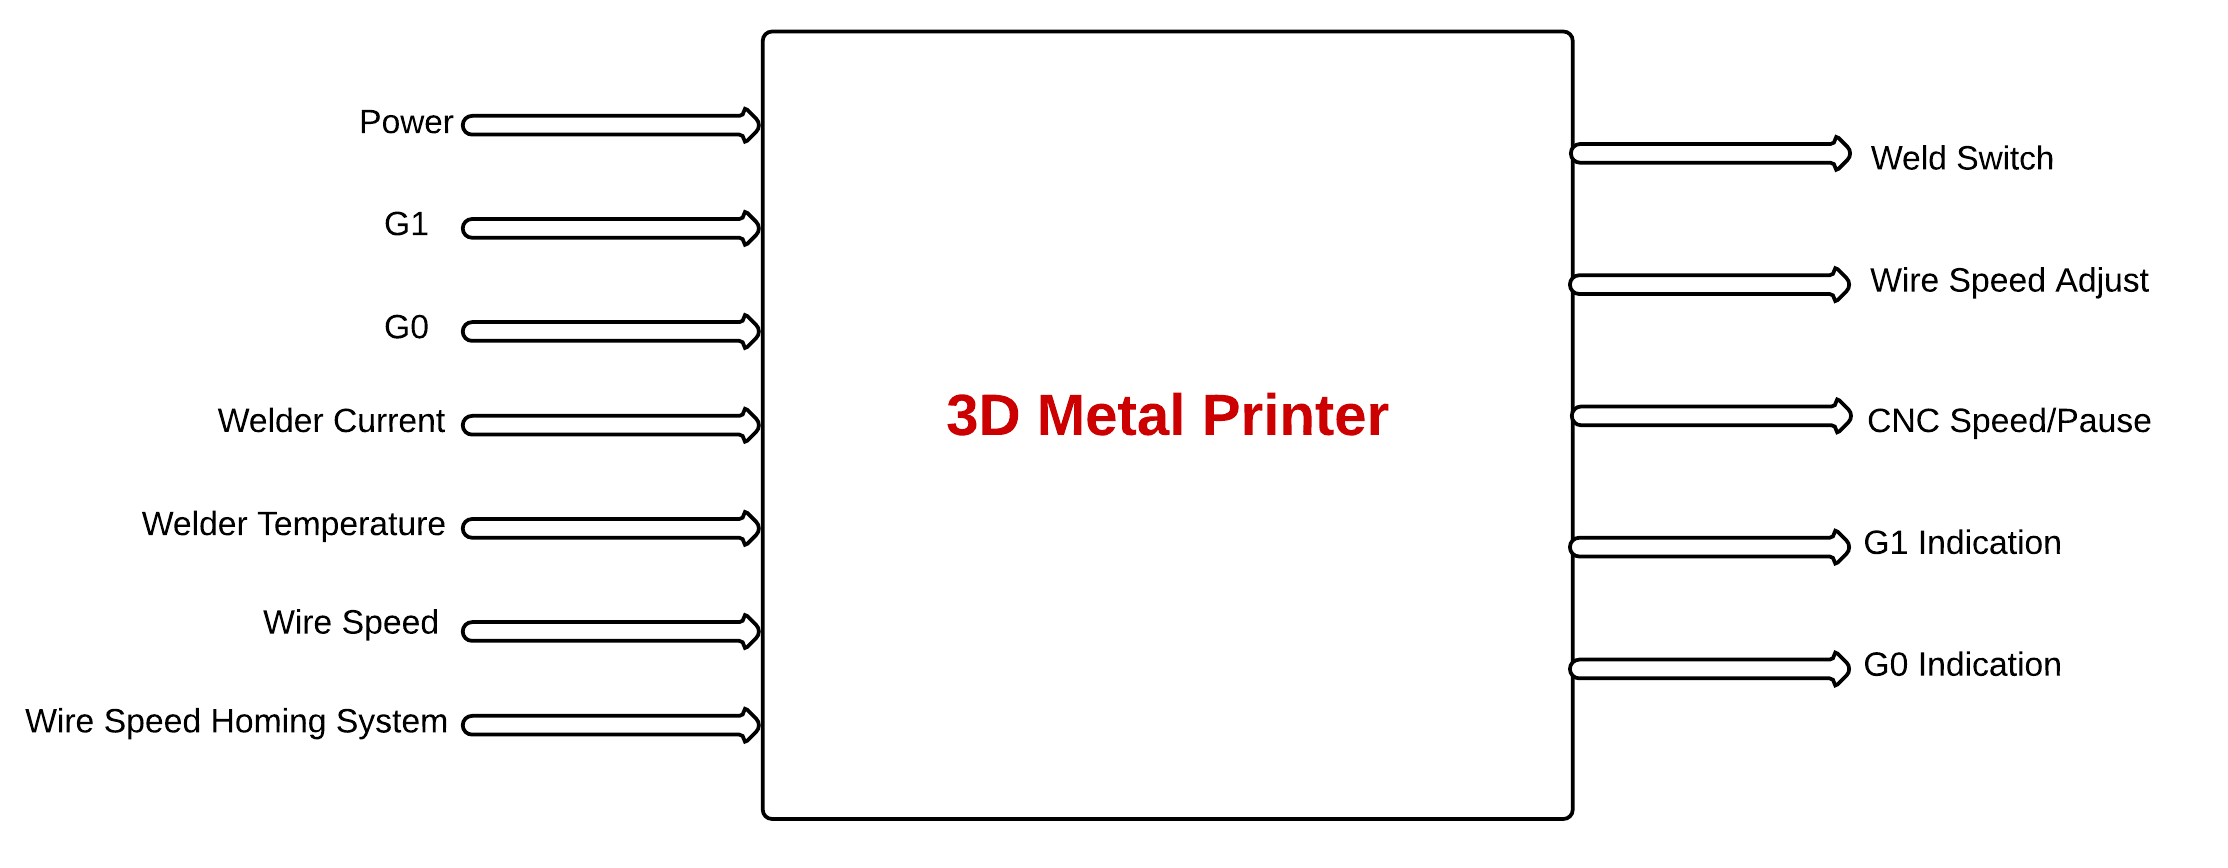
\includegraphics[scale=0.9]{mainfc}
\caption{Level-0 Block Diagram of the 3D Metal Printer}
\end{figure}

\clearpage

\begin{figure}[h]
\centering
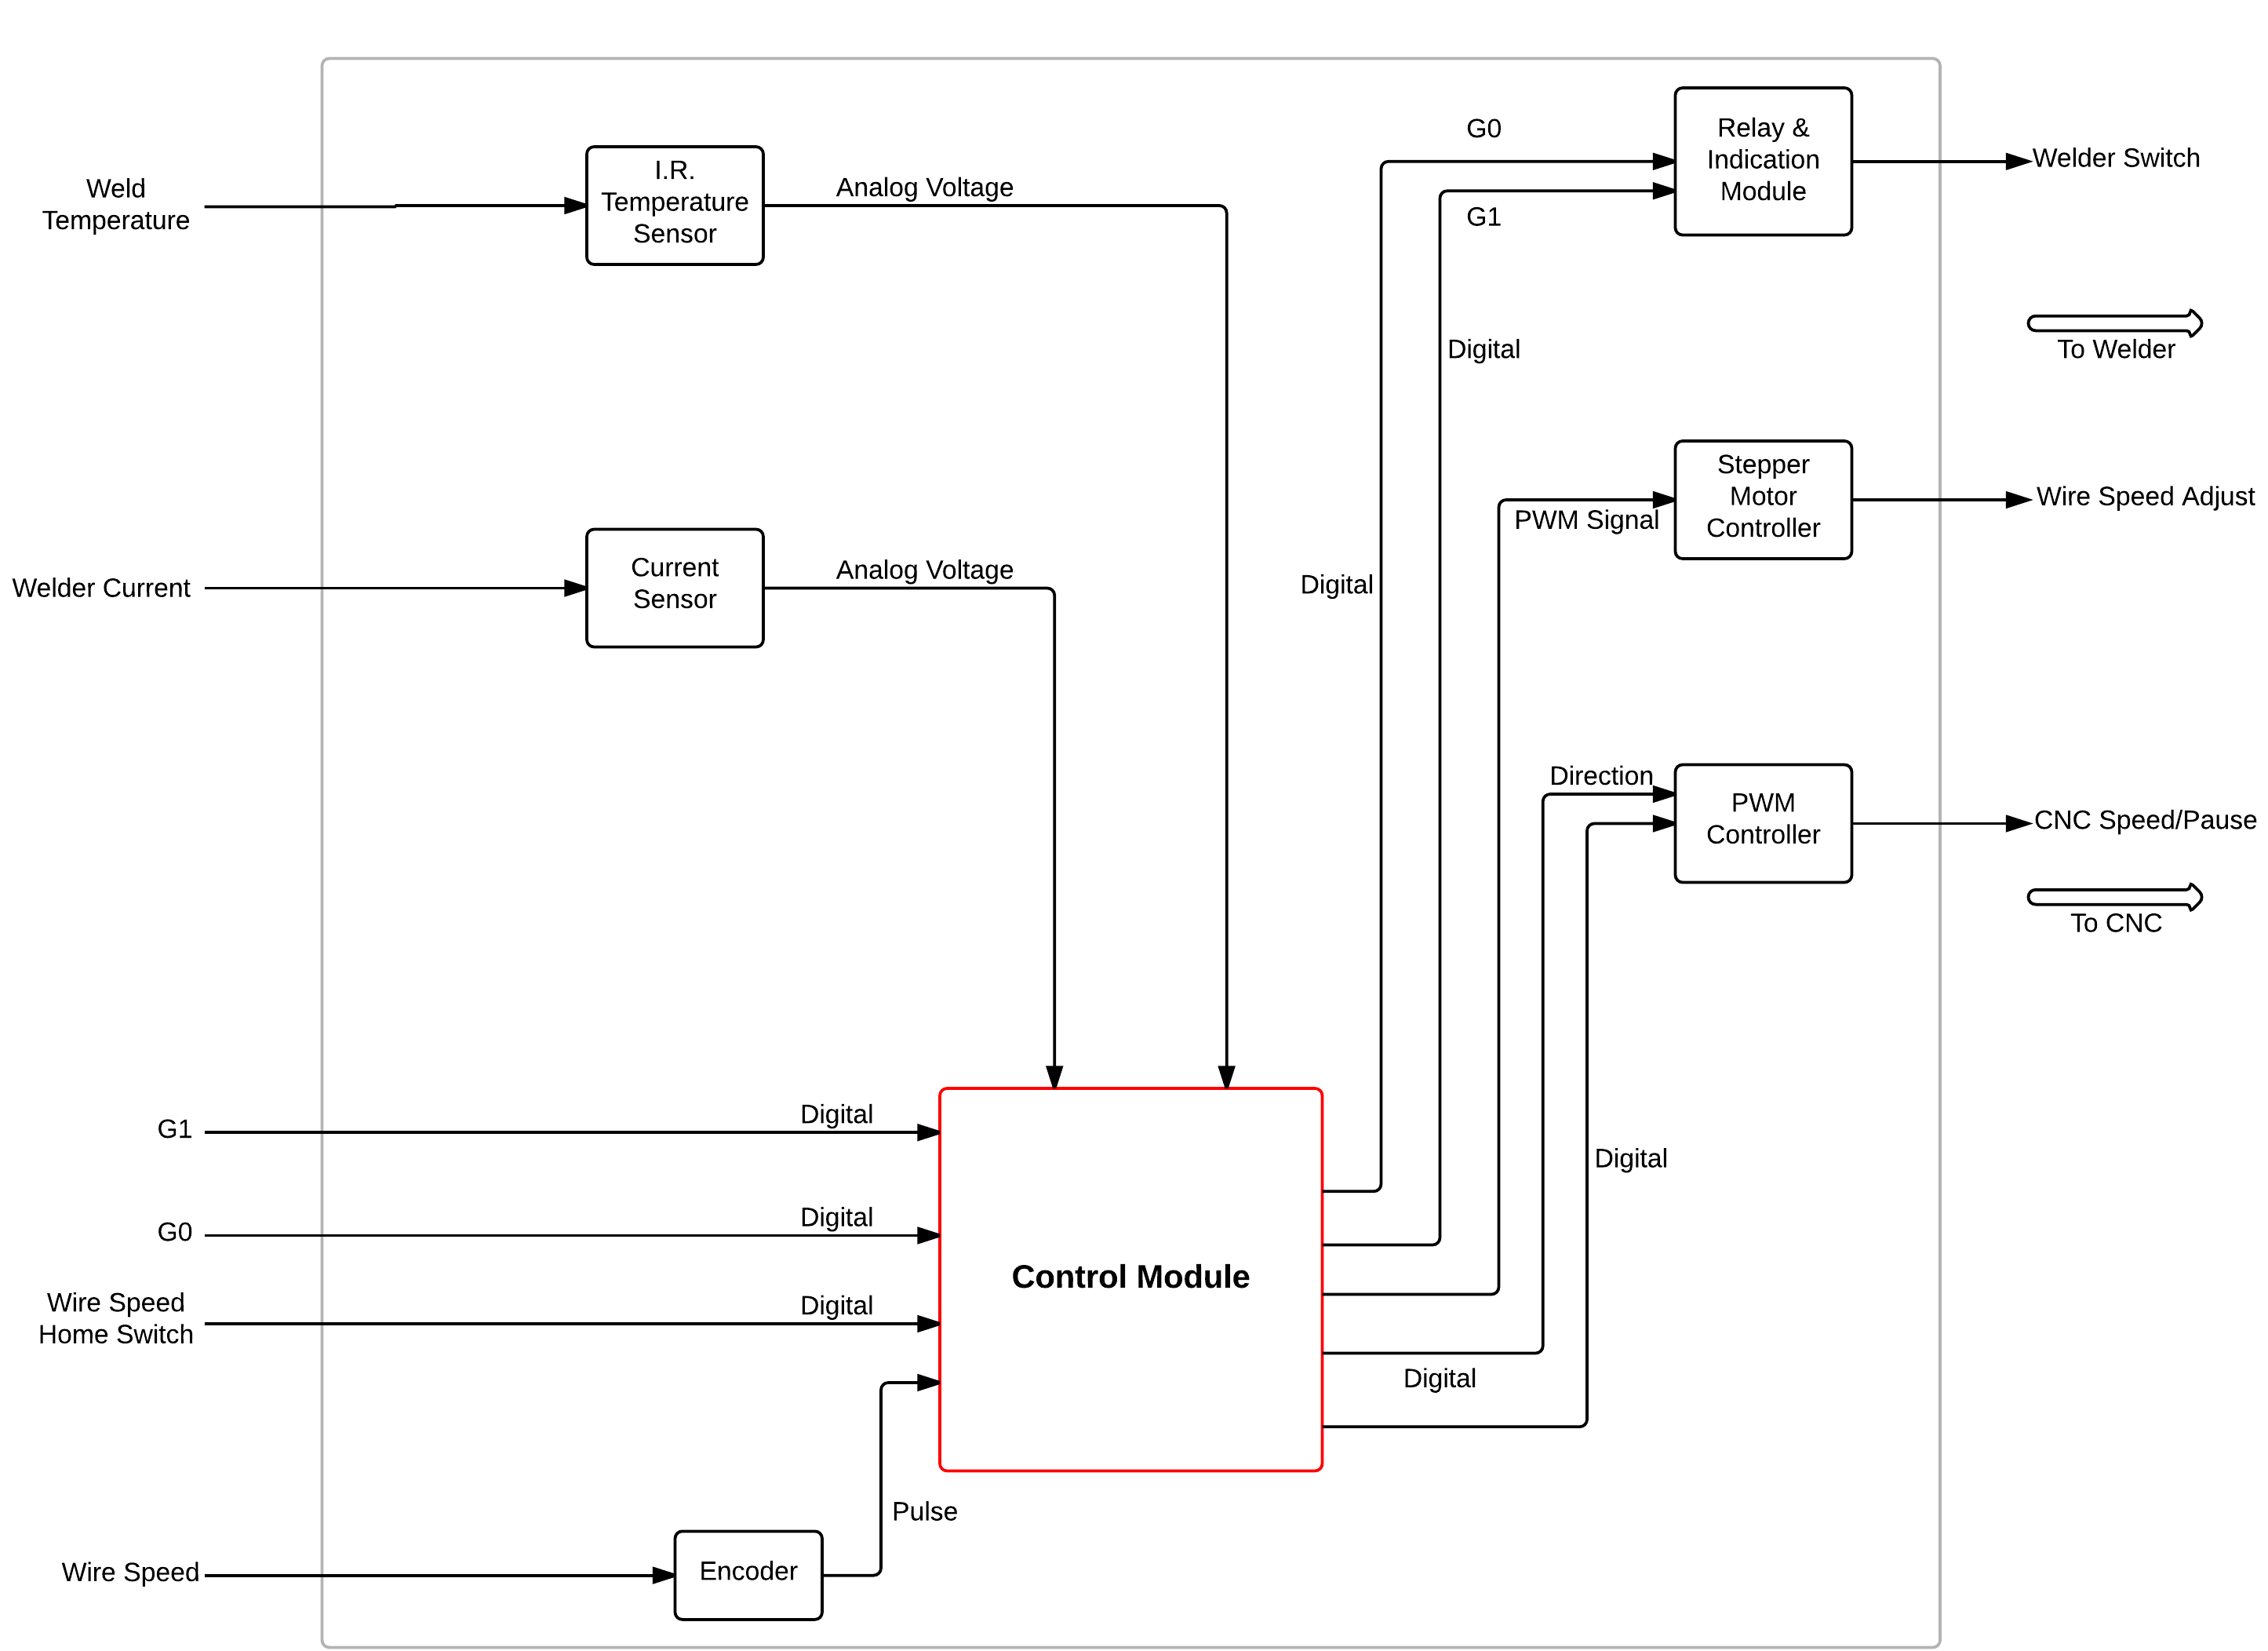
\includegraphics[scale=0.655,angle=90]{detailedflo}
\caption{Level-1 Block Diagram of the 3D Metal Printer}
\end{figure}

\clearpage

\section{Schedule}

\begin{figure}[!h]
\centering
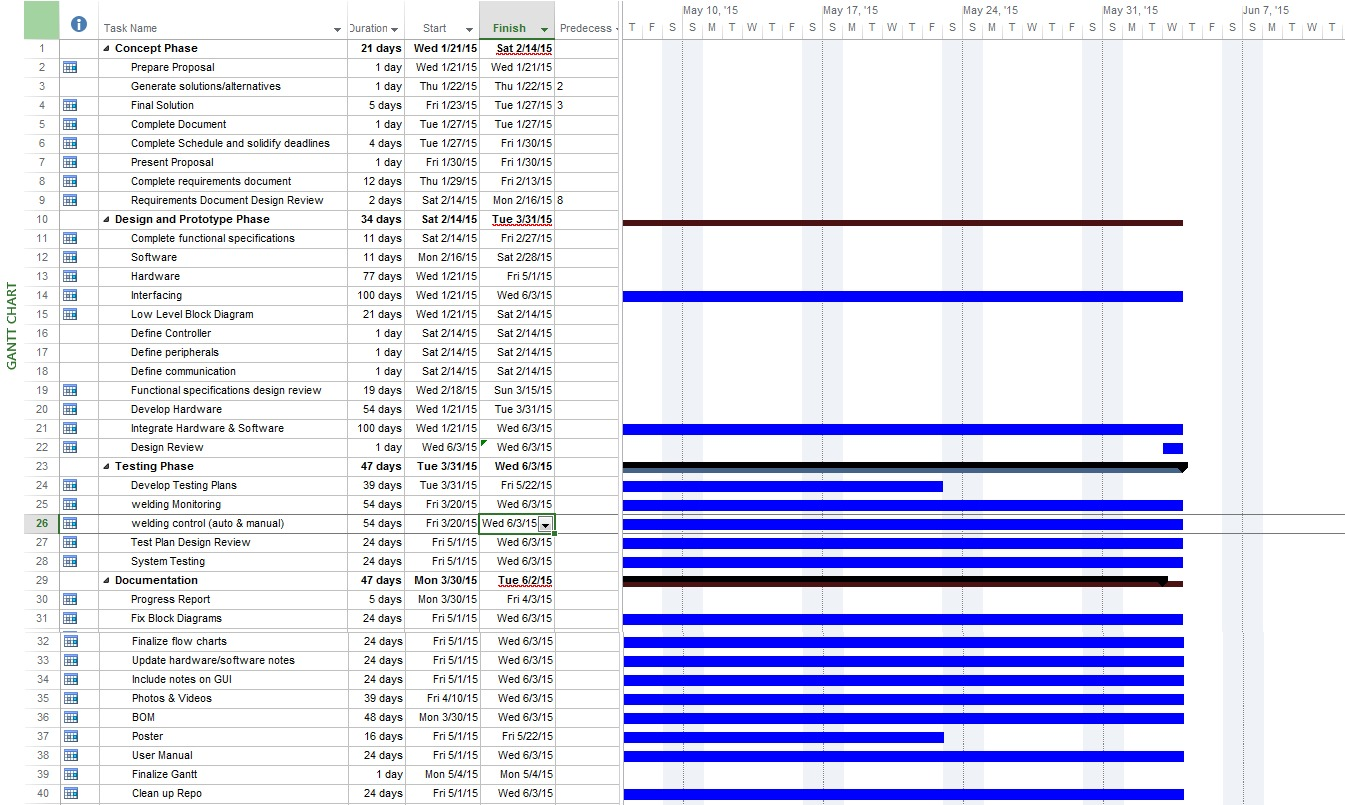
\includegraphics[scale=0.43,angle=90]{finalganttchart}
\caption{Gantt Chart showing the schedule}
\end{figure}

\clearpage

\section{Hardware}

\subsection{Welder Control}

\indent To control the welder, a central control module will be used. This was a hot topic of debate for several weeks, as the number of choices available for this project are very high. The sponsor's requirements for the project was that all of the control work was done by a separate computer from the one used by Linux CNC, this only narrowed it down to a choice between a PCIe DAC board and a single board computer. Based on the need for both analog and digital control pins and the need for future expansion, we researched and came up with several options.


\begin{center}


\begin{tabular}{ |c | c | }


  \hline
  \textbf{Single Board Computers} & \textbf{DAC} \\ \hline            
  Raspberry-Pi & Sensoray 826 \\ \hline      
  Intel Galileo & MCC DAS1602/16  \\ \hline      
  SBC 8600B &  \\ \hline
    Wander Board Solo &  \\ \hline
      Beagle Bone Black &  \\ \hline
\end{tabular}
\end{center}


\indent In the end we chose the Sensoray 826 board because for the price it outperforms all other boards on the market by having 16 analog inputs, 8 analog outputs, and 48 digital I/O pins. This board was chosen for the high level of future expandability that it has, and because it is a PCIe card which can be packaged into its own desktop as per request from the sponsor.\



To control the current to the weld and the wire speed of the welder, two stepper motors have been fitted to the  manual control knobs, and are connected to a motor driver module. The Sensoray board will be controlling the motor drivers using a sequence of rising and falling edges. To allow the controller board to control at what time the welder is depositing and when it is not depositing, a relay with a transistor driver will be used.\\




\indent The signal that tells the controller will be coming from the CNC machine's I/O card. It is a switch type signal which means that when the signal is sent, an internal switch will be closed, causing what ever is on the input to be shown on the output. The CNC machine uses G-Code (described below), and Linux CNC allows outputs to be asserted when a particular G-Code instruction is executed. G1 and G0 are going to be used to tell the I/O card to close and open the switch, which will assert 5V DC to the input to the control module. The control module will assert an output high or low which will open or close the welder switch, turning the welder on and off.\\ 

\indent The Sensoray 826 I/O card has three 50 pin connectors and two 26 pin connectors. To allow easy access to these pins, a breakout board with screw terminals has been made so that wires can easily be disconnected and switched.

\clearpage

\subsection{Breakout Boards}

\indent To easily connect to the Sensoray 826 board, several breakout boards with screw terminals were made. There are two types of break out boards, a 50-pin board and a 26-pin board. 50 pin boards are used to connect to the digital and analog pins of the control board, while 26 pin boards are used to connect to the various counter channels. Shown below are mages of the boards them selves. With the empty side of the board facing you, the screw terminals are in order from 1 to 50/26 starting on the right hand side. \\


\begin{figure}[!h]
\centering
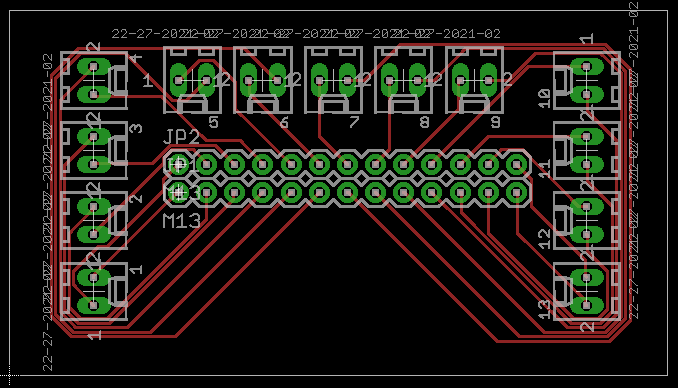
\includegraphics[scale=0.5]{26}
\caption{Board Layout of the 26 pin Breakout Board for the Sensoray 826 I/O card}
\end{figure}



\begin{figure}[!h]
\centering
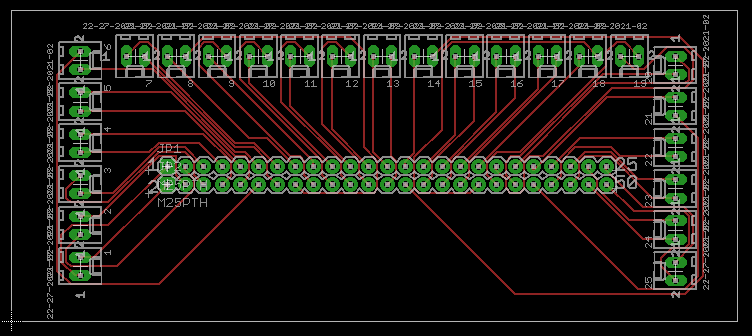
\includegraphics[scale=0.55]{50}
\caption{Board Layout of the 50 pin Breakout Board for the Sensoray 826 I/O card}
\end{figure}

\clearpage

\begin{figure}[!h]
\centering
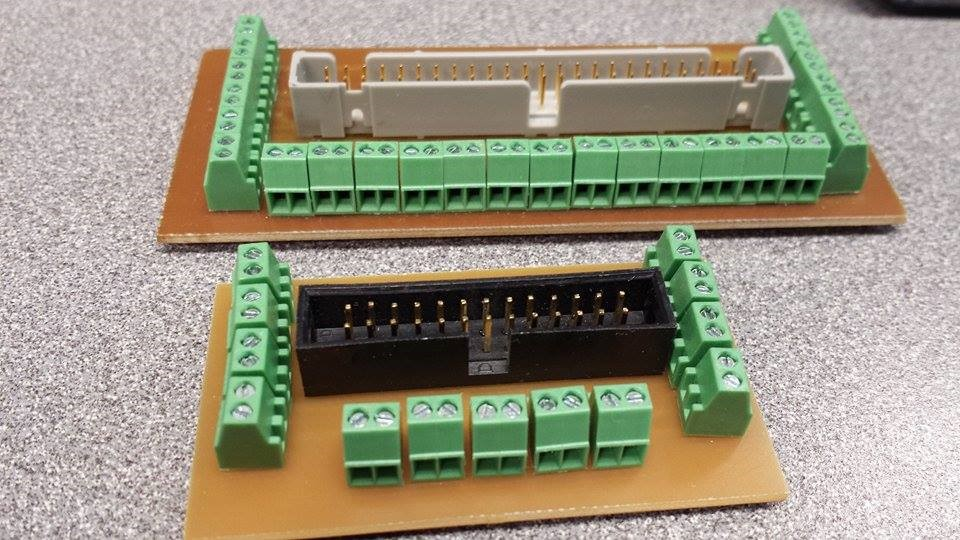
\includegraphics[scale=0.5]{realbreaker}
\caption{The 26 and 50 pin Breakout Boards with connectors for The Sensoray 826 I/O card}
\end{figure}

\subsection{Temperature Sensor}

An infrared temperature sensor will be used to measure the temperature surrounding the weld area. These temperature sensors typically have a higher operating range than other types of temperature sensors. The chosen sensor is the CTLM-1M-1H1-CTL-CF4 from Micro-Epsilon. This sensor was chosen of it’s operating range was 800C to 2200C. It has multiple configurable output types, including current output, voltage output, and alarm outputs. This sensor also has a focus point at 450mm (\~18 in) which gives considerable distance from the weld, and it is not impractically far away. Further documentation can be found (Appendix temp sens). The Sponsor has agreed to take care of mounting the sensor on the machine.\\

The chosen output type of the temperature sensor is chosen to be a voltage output with a full-scale range of 0V to 10V. This range was chosen because the ADC on the Sensoray 826 are configurable to accept up to +10V and another Analog input needed the input configured to +10V. Setting the output range to 0V-10V on the current sensor removed the need to write additional software to solve an issue that was solved in other means.

\clearpage

\begin{figure}[!h]
\centering
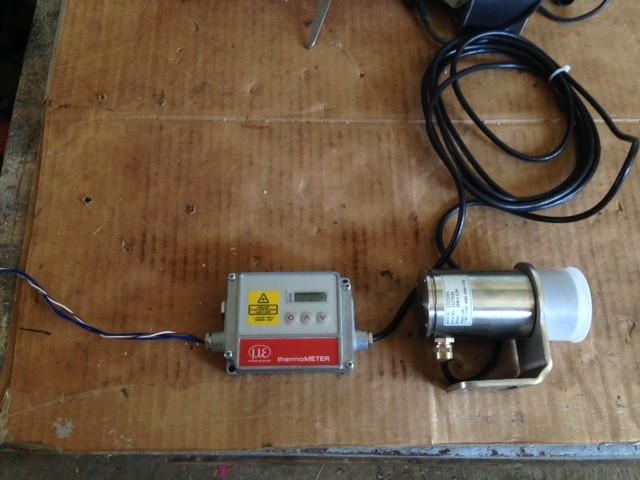
\includegraphics[scale=0.5]{tempsensor}
\caption{The Micro-Epsilon 1MH1-CF4 Temperature Sensor}
\end{figure}

\subsection{Incremental Encoder}

The Incremental Encoder is used to measure the actual wire speed of the welder wire. The encoder needed to be incremental because of the need to know speed, and that current position did not matter. The chosen encoder is the U.S. Digital S5-5000-250-IE-D-B. Initially a pulley on a shaft type encoder was going to be used. The pulley be mounted to the frame of the welder and the encoder would be placed under tension underneath the wire that is being fed to the weld. However this was not successful as there could not be any external tension placed on the wire inside the welder.\\

Fortunately the main drive pulley has a square drive shaft and stuck out past the edge of the pulley. A small plastic “coupler” piece was 3D printed that adapted the round end of the encoder, to the square drive shaft of the drive pulley. The CAD drawing of this part can be seen to the left. This piece allowed an accurate measurement of the actual wire speed of the welder to be interpreted by the Sensoray 826. Here, the calculations for the wire speed can be found.

\clearpage

\begin{figure}[!h]
\centering
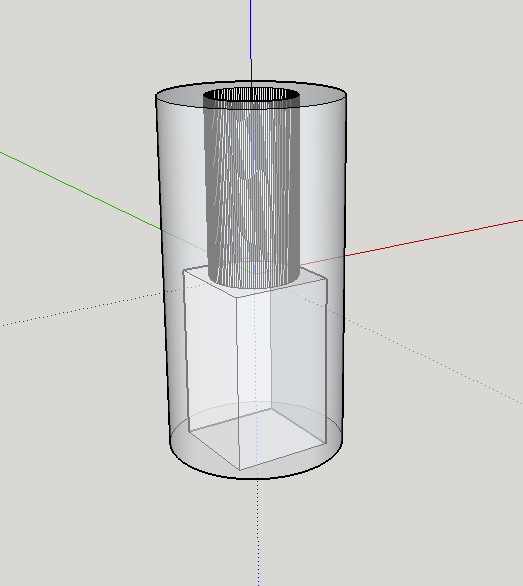
\includegraphics[scale=0.5]{enc}
\caption{Schematic of the Incremental Encoder}
\end{figure}

\begin{figure}[!h]
\centering
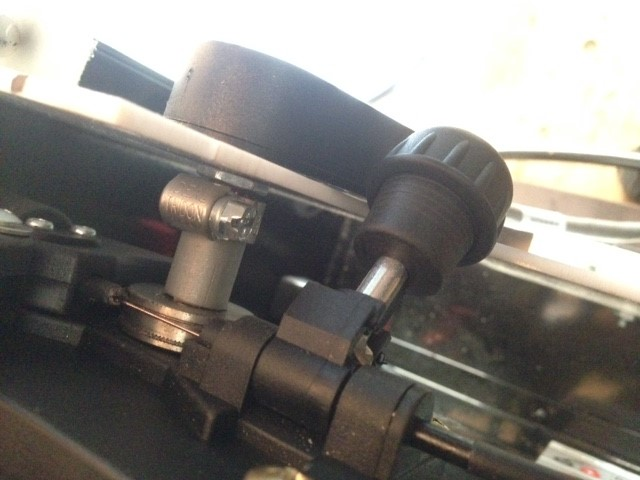
\includegraphics[scale=0.5]{encreal}
\caption{The US Digital S5-5000-250-IE-D-B Incremental Encoder}
\end{figure}

\clearpage

\subsection{Relay and Indication Module}

\indent A relay was used to interface the Sensoray 826 with the welder. A relay provides isolation from any harmful voltage spike that occurs on the welder’s circuit. It also acts as a mechanical switch, which is the same as the trigger on the welder gun itself. It is unknown what type of signal is passed through the welder switch weather its DC, or AC the relay will on act differently, as a transistor might. The interface circuit includes a transistor drive circuit that switches an 8V supply (which comes from a wall wart power supply) across the coil of the relay on and off. This module also includes LEDs to indicate what state the CNC machine is currently in. A schematic and an image of the final module can be seen below.

\indent There were some issues with the relay module, where were that the Sensoray 826 has internal 10k pull up resistors, and when the machine powers up, the active low DIO pins are initialized to a 0-state, which means that the voltage is high on the pin. When connected to the welder, this meant that when there was not any code being executed the welder would be activated. To remedy this issue, an inverter was placed on the input.\\


\begin{figure}[!h]
\centering
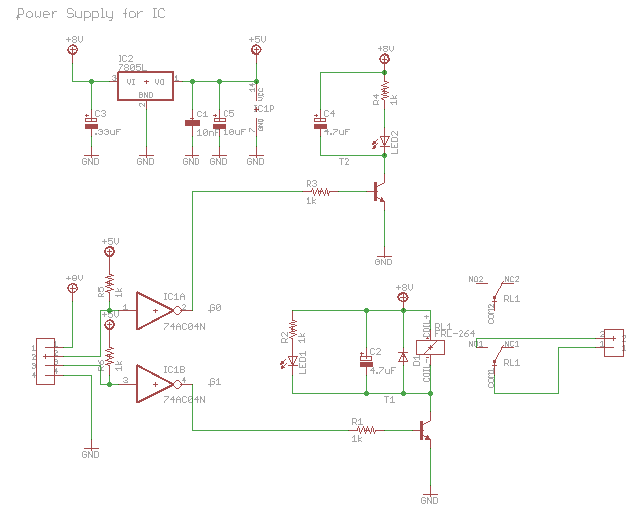
\includegraphics[scale=0.8]{relay11}
\caption{Schematic of the Relay \& Indication Module}
\end{figure}

\clearpage


\begin{figure}[!h]
\centering
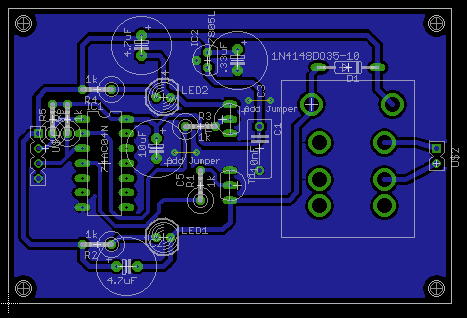
\includegraphics[scale=1]{relayboard}
\caption{Board Layout of the Relay \& Indication Module}
\end{figure}

\begin{figure}[!h]
\centering
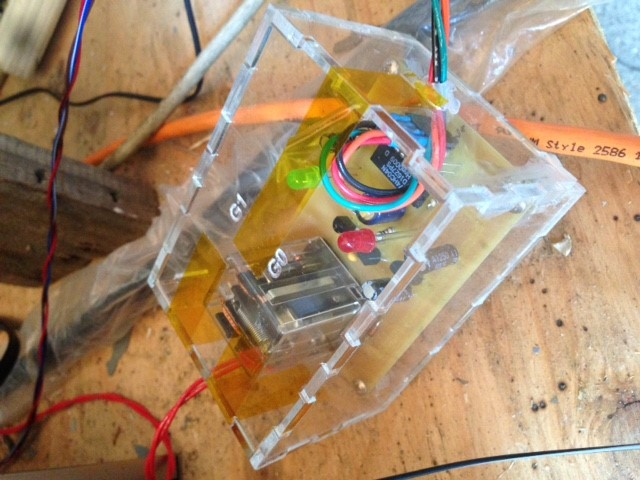
\includegraphics[scale=0.55]{relayreal}
\caption{The Relay \& Indication Module}
\end{figure}

\clearpage

\subsection{Stepper Motor Controller}

\textbf{P/N:} \\
\textbf{Controller:} KL-5056 \\
\textbf{Motor:} KL23H2100-35-4B \\

\indent The stepper motor controller is used to control a motor that adjusts the wire speed knob on the welder. From the Sensoray 826, there are two digital signals that control how much and in which direction the motor turns. To tell the motor two turn, a PWM signal with a 50\% duty cycle is used. The frequency determines the speed of rotation. The direction signal is either a high or low 5V signal that will turn the motor clockwise or counterclockwise. The controller also has a programmable step resolution, which is either defined in software, or by using the DIP switched located on the side of the controller. Further documentation on the controller can be found here. \\
\indent The motor is coupled to the wire speed adjustment knob via a PVC cylinder, which have elevated surfaces where the limits of the knob are. Shown below, are switches that get triggered if the motor turns too far. The limit switches are connected to the enable pin of the motor controller, so that if the motor accidentally turns too far, it will disable its self and it will not damage the knob on the welder. An additional switch is added to the PVC cylinder, which is used as a reference position of the knob. Shown below is the wiring diagram of the motor controller.


\begin{figure}[!h]
\centering
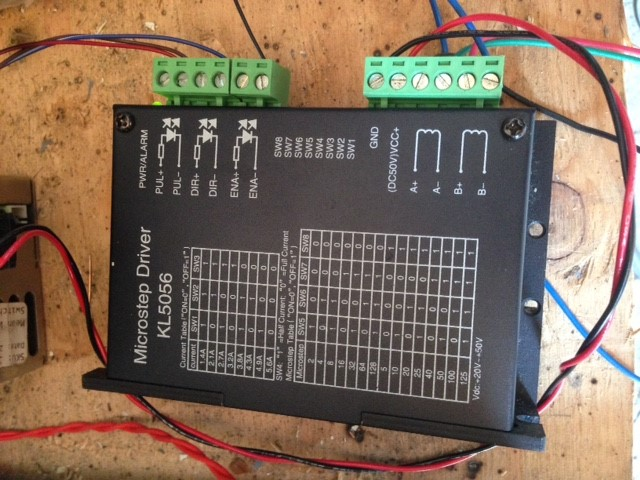
\includegraphics[scale=0.55]{stepper}
\caption{The Stepper Motor Controller}
\end{figure}


\clearpage
\subsection{PWM Controller}

\textbf{P/N:} Mesa THC A-D \\

The PWM controller is a voltage to frequency converter. It is used to externally start and stop the CNC machine. The voltage input of the PWM controller is connected to a digital output of the Sensoray 826. To stop the CNC Machine, a 5V signal is send and to stop it is 0V. The CNC machine is initialized to use this 5V signal in the .HAL file associated with that machine. In fact the voltage on that pin can be anywhere between 0V and 5V for further external control of the welder, however in the scope of this project, only a high or low signal needs to be sent.

\begin{figure}[!h]
\centering
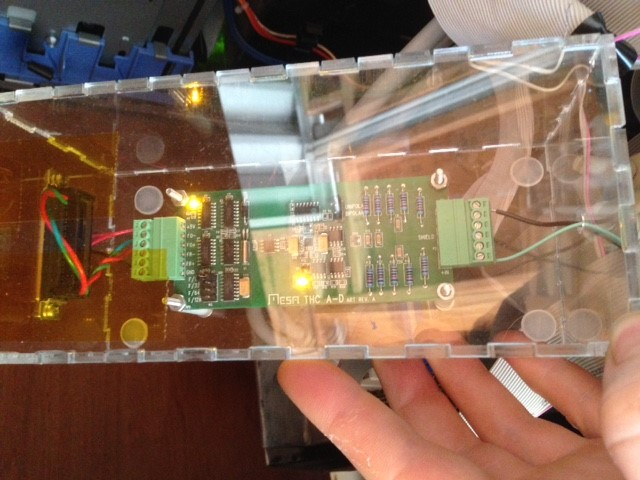
\includegraphics[scale=0.55]{pm}
\caption{The Mesa THC A-D PWM controller}
\end{figure}


\clearpage


\subsection{Current Sensor}

\textbf{P/N:} CSLA1DJ \\

This current sensor has an operational range of 0 to 225A, which is well over the maximum current of the welder. It is placed in a small plastic housing, which a jumper cable is passed though. The sensor is a Hall effect sensor that is placed inside a ferrite toroid. The output of the sensor is a voltage that sits at half of the supply voltage, and will deviate above or below that level based on he magnitude and direction of the current. There is a metal lug, which the ground connection of the welder connects to. The other end of the module is a large alligator clamp that connects to the plate being welded to.


\begin{figure}[!h]
\centering
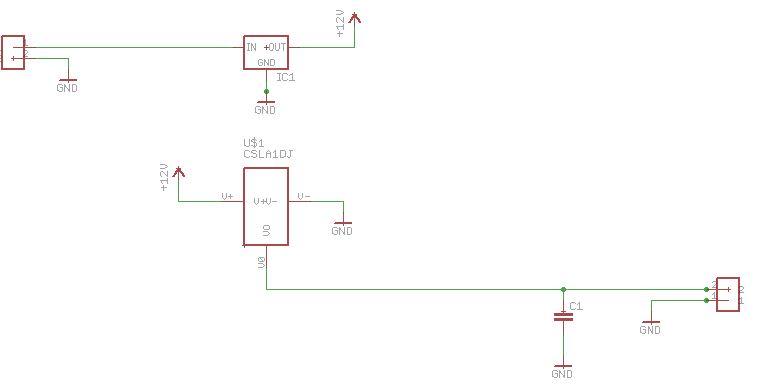
\includegraphics[scale=0.6]{currentsensor}
\caption{Schematic of the Current Sensor}
\end{figure}

\begin{figure}[!h]
\centering
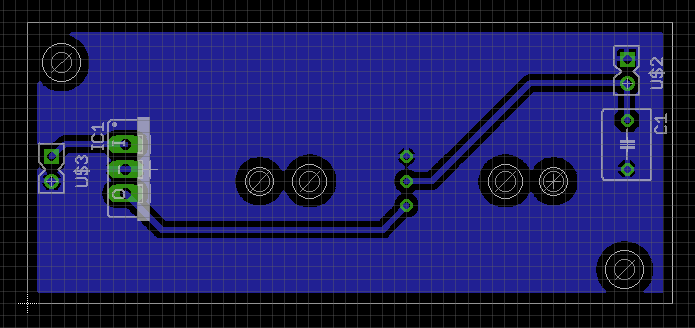
\includegraphics[scale=0.7]{currentboard}
\caption{Board Layout of the Current Sensor}
\end{figure}


\clearpage


\begin{figure}[!h]
\centering
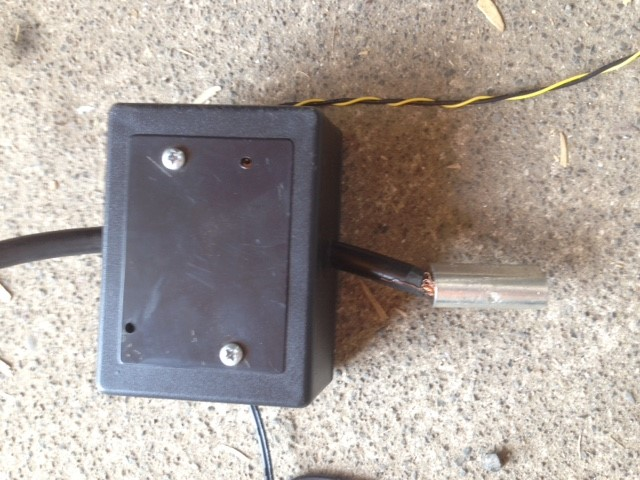
\includegraphics[scale=0.55]{currentreal}
\caption{The CSLA1DJ Current Sensor}
\end{figure}

\clearpage

\subsection{Wire Speed}

%\begin{itemize}

\textbf{For calculating Wire Speed with Rotary Encoder}\\

\begin{figure}[h]
\centering
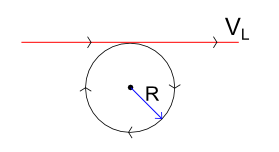
\includegraphics[scale=0.7]{speed1}
\end{figure}


So Angular Velocity is,

\begin{center}



$\boldsymbol{\displaystyle f=\frac{n}{\displaystyle Nt}}$\\
\end{center}

$n$ = number of up/down counts, $N$ = number of up/down counts/rev, $T$ = sampling time.\\


And Linear Velocity is,

\begin{center}



$\displaystyle v_L = \omega r$\\
$\displaystyle \omega = 2 \pi f $
\end{center}

So,

\begin{center}



$\boldsymbol{\displaystyle V = \frac{\pi nd}{NT}}$ \\

\end{center}



\textbf{Connections to 826}\\
\begin{center}


\begin{tabular}{c|c|c}
J\textsubscript{4} & Pin 1 & +A0 \\
& Pin 2 & -A0 \\
& Pin 3 & GND \\
& Pin 4 & +B0 \\
& Pin 5 & -B0 \\
\end{tabular}
\end{center}

\clearpage

\begin{figure}[h]
\centering
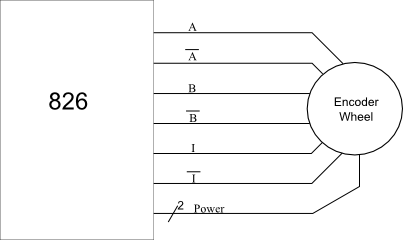
\includegraphics[scale=0.8]{connections}
\caption{Encoder Connection}
\end{figure}


\subsection{Pin Assignments}

\begin{adjustwidth}{-2cm}{-2cm}


\begin{center}


\begin{tabular}{ |c|c|c|c| }


  \hline
  \thead{DIO \\ PINS} & \textbf{Wire Color} & \thead{Channel \\ Number} & \textbf{Function} \\ \hline
      
1 &	Teal &	23 &	CNC Start/Stop \\ \hline
2 &	Black &	&	GND for CNC Start/Stop \\ \hline
3 &	Blue with White Stripe &	22 &	Direction of Stepper Motor \\ \hline
4 &	Black with White Stripe &	 &	Return path for Limit Switch \\ \hline
5 &	Brown &	21 &	Pulse on Motor Controller \\ \hline
6 &	N/C & &		GND \\ \hline
7 &	Purple &	20 &	Wire Speed Home Switch \\ \hline
8 &	Black & &		GND for Wire Speed Home Switch \\ \hline
9 &	Green with White Stripe &	19 &	G1 Input (From CNC Machine) \\ \hline
10 &	N/C & &		GND \\ \hline
11 &	Orange with White Stripe &	18 &	G0 Input (From CNC Machine) \\ \hline
12 &	N/C & &		GND \\ \hline
13 &	Green &	17 &	G1 Output (To Relay and Ind. Module) \\ \hline
14 &	Black & &		GND for Relay Module \\ \hline
15 &	Orange &	16 &	G0 Output (To Relay and Ind. Module) \\ \hline
16 &	Black & &		Power Supply GND for Relay Module \\ \hline
17 & &		15	 & \\ \hline
18 & & 			& GND \\ \hline
19 & &		14 & \\ \hline	
20 & &			& GND \\ \hline
21 & &		13 & \\ \hline	
22 & &			& GND \\ \hline
23 & &		12 & \\ \hline	
24 & &			& GND \\ \hline
25 & &		11 & \\ \hline	



  
\end{tabular}





\end{center}

\end{adjustwidth}

\clearpage


\begin{adjustwidth}{-2cm}{-2cm}

\begin{center}


\begin{tabular}{ |c|c|c|c| }


  \hline
  \thead{DIO \\ PINS} & \textbf{Wire Color} & \thead{Channel \\ Number} & \textbf{Function} \\ \hline
      

26 & &			& GND \\ \hline
27 & &		10 & \\ \hline	
28 & &			& GND \\ \hline
29 & &		9 & \\ \hline	
30 & &			& GND \\ \hline
31 & &		8 & \\ \hline	
32 & &			& GND \\ \hline
33 & &		7 & \\ \hline	
34 & &			& GND \\ \hline
35 & &		6 & \\ \hline	
36 & &			& GND \\ \hline
37 & &		5 & \\ \hline	
38 & &			& GND \\ \hline
39 & &		4 & \\ \hline	
40 & &			& GND \\ \hline
41 & &		3 & \\ \hline	
42 & &			& GND \\ \hline
43 & &		2 & \\ \hline	

44 & &			& GND \\ \hline
45 & &		1 & \\ \hline	
46 & &			& GND \\ \hline
47 & &		0 & \\ \hline	
48 & &			& GND \\ \hline
49 & &		 &  5V to the CNC Switching system and Motor Controller \\ \hline	
50 & &			& GND \\ \hline




  
\end{tabular}



\end{center}

\end{adjustwidth}

\clearpage




%\begin{adjustwidth}{-2cm}{-2cm}


\begin{center}


\begin{tabular}{ |c|c|c|c| }


  \hline
  \thead{ANALOG \\ PINS} & \textbf{Wire Color} & \thead{Channel \\ Number} & \textbf{Function} \\ \hline
      
1 &	& &	 \\ \hline
2 &	& &	 \\ \hline
3 &	Black &	0 &	GND for Current Sensor \\ \hline
4 &	Yellow &	0 &	Current Sensor Signal \\ \hline
5 &	Black &	1 &	GND for Temperature Sensor \\ \hline
6 &	Grey &	1 &	Temperature Sensor Signal \\ \hline

7 &	& & \\ \hline
8 &	& & \\ \hline
9 &	& & \\ \hline
10 &	& & \\ \hline
11 &	& & \\ \hline
12 &	& & \\ \hline
13 &	& & \\ \hline
14 &	& & \\ \hline
15 &	& & \\ \hline
16 &	& & \\ \hline
17 &	& & \\ \hline
18 &	& & \\ \hline
19 &	& & \\ \hline	
20 &	& & \\ \hline
21 &	& & \\ \hline
22 &	& & \\ \hline
23 &	& & \\ \hline
24 &	& & \\ \hline
25 &	& & \\ \hline
26 &	& & \\ \hline
27 &	& & \\ \hline
28 &	& & \\ \hline
29 &	& & \\ \hline
30 &	& & \\ \hline
31 &	& & \\ \hline
32 &	& & \\ \hline
33 &	& & \\ \hline
34 &	& & \\ \hline
35 &	& & \\ \hline
36 &	& & \\ \hline
37 &	& & \\ \hline
38 &	& & \\ \hline
39 &	& & \\ \hline
40 &	& & \\ \hline



  
\end{tabular}





\end{center}

%\end{adjustwidth}

\clearpage


\begin{center}


\begin{tabular}{ |c|c|c|c| }


  \hline
  \thead{ANALOG \\ PINS} & \textbf{Wire Color} & \thead{Channel \\ Number} & \textbf{Function} \\ \hline
      
41 &	& & \\ \hline
42 &	& & \\ \hline
43 &	& & \\ \hline
44 &	& & \\ \hline
45 &	& & \\ \hline
46 &	& & \\ \hline
47 &	& & \\ \hline
48 &	& & \\ \hline
49 &	& & \\ \hline
50 &	& & \\ \hline


  
\end{tabular}





\end{center}



\begin{center}


\begin{tabular}{ |c|c|c|c| }


  \hline
  \thead{COUNTER \\ PINS} & \textbf{Wire Color} & \thead{Counter \\ Channel \\ Number} & \textbf{Function} \\ \hline
      
1	& Blue with White dots &	0 &	A+ on Encoder \\ \hline
2	& White with Blue dots &	0 &	A- on Encoder \\ \hline
3	& \makecell{Green with White dots \\ (note cable shield also connected)} &	0 &	GND on Encoder \\ \hline
4	& Brown with White dots &	0 &	B+ on Encoder \\ \hline
5	& White with Brown dots &	0 &	B- on Encoder \\ \hline
6	& White with Green dots & 	0 &	POWER on Encoder \\ \hline
7	& Orange with White dots &	0 &	I+ on Encoder \\ \hline
8	& White with Orange dots &	0 &	I- on Encoder \\ \hline
9 &	& & \\ \hline
10 &	& & \\ \hline
11 &	& & \\ \hline
12 &	& & \\ \hline
13 &	& & \\ \hline
14 &	& & \\ \hline
15 &	& & \\ \hline
16 &	& & \\ \hline
17 &	& & \\ \hline
18 &	& & \\ \hline
19 &	& & \\ \hline	
20 &	& & \\ \hline
21 &	& & \\ \hline
22 &	& & \\ \hline
23 &	& & \\ \hline
24 &	& & \\ \hline
25 &	& & \\ \hline
26 &	& & \\ \hline

  
\end{tabular}





\end{center}

\clearpage



\section{Software}

\subsection{Software Description}

\indent The main program for our control system was written entirely in  the programming language "C". This was chosen so as to ensure compatibility with the Sensoray 826 DAQ board used for control. The program begins by asking the user to disconnect the grounding cable of the welder and waiting for an input from the user confirming this task is completed. Upon receiving that input the machine then runs a calibration procedure by running a PWM procedure to turn the stepper motor until the system sees the homing switch is triggered. The program then turns on the welder's gun to feed wire while measuring  the wire speed and setting the average of those wire speeds as the new homing offset. \\
\indent	The next step of the program asks the user to input the speed the CNC machine will be running at for the duration of the print in in/sec. It uses this value to find a corresponding nominal wire speed in an array of nominal wire speeds found via testing, and sets the welding machine to that wire speed. The program then waits for a signal from the CNC machine that it has switched from Relocation mode to Deposition mode. Once the system sees that we have reached Deposition mode, it stops the CNC movement and makes sure the welder is not triggered, in order to check the temperature of the base plate being welded to. If the base plate's temperature is too low the system will pause and wait for a torch to heat the base plate up to above a given threshold value. \\
\indent	On completion of the torch routine the system enters the main loop, this begins by reading a timestamp from the 826's onboard timestamp generator, this value in microseconds will be used to keep track of how long the machine has been in deposition mode later. The system then starts the welder and runs a check for spikes in the current seen by the Current Sensor, if it sees none the system will end the program and return an error report, otherwise the program moves on and starts the CNC's movement back up so that we can check if the machine is still in Deposition mode. If the CNC machine is still in Deposition mode at that time it moves on to take measurements of the number of "peaks" seen by the current sensor, the temperature of the weld's base plate, and  the incremental encoder used to measure wire speed. Amongst the measurements it checks and updates the mode of movement seen by the CNC in order to avoid issues with our system trying to deposit while in Relocation mode. \\
\indent	At the end of checking all sensor measurements, the system begins comparing the observed value with the pre-programmed threshold values. The first check is to make sure that the current plate temperature is at an acceptable value. If the temperature has fallen or risen too far, the whole system stops, and runs the torch routine before starting the system back at the initial timestamp read. If the temperature is at an acceptable value, the average droplet spacing is checked against a nominal value found through testing. If the error between the two values is greater or less than 20\%, the system terminates with an error, asking the user to double check that the entire system is working. The last check is to see if the droplet spacing is greater or less than a 5\% tolerance, and if so the system makes an appropriate proportional adjustment to the wire speed before continuing on.

\subsection{G-Code}

\indent G-code is the commonly used name to refer to a numerical programming language. As is the case with all languages, G-code has its own syntax and semantics.  A line of code is referred to as a block, and a program is defined as multiple blocks. All programs start and end with the percent symbol (\%). While writing G-code, the backslash (/) can be used to comment out an entire line, whereas if you want to make comments about a block, parentheses are to be used. Anything inside of a set of parentheses will be ignored by the compiler. As is the case with most other languages, G-code ignores white space, so spacing is used to clarify the code for the writer as well as future users.

\indent All points of G code are comprised of words and numbers. A word is simply a letter. For example, the block “X0” is simply the word X and the value 0. The words X, Y, and Z refer to the three axes, while the G words refer to the movement, motion, and location. When first started up, any blocks of code will use the point (0,0,0) as home, however G54 establishes a new temporary “home” point and G52 establishes the point where the temporary reference point is to be set. In other words, the block of code “G54 G52 X100 Y100 Z0” changes the reference point from (0,0,0) to (100,100,0) and the remainder of the code will run from this point, unless a new reference point is defined.

\indent Similarly, other G-code words can be used to define how the space between two points should be interpolated. In some instances you may want two points to be connected via a straight line, while at other times it would be better to have them connected via a circular pattern. When dealing with circular interpolation, you can set it to be done in either a clockwise or counterclockwise manner. Beyond just linear and circular interpolation, there are dozens of G-code words that determine how the code is to be run (Appendix C). 

\clearpage

\subsection{Control Program}

\begin{figure}[!h]
\centering
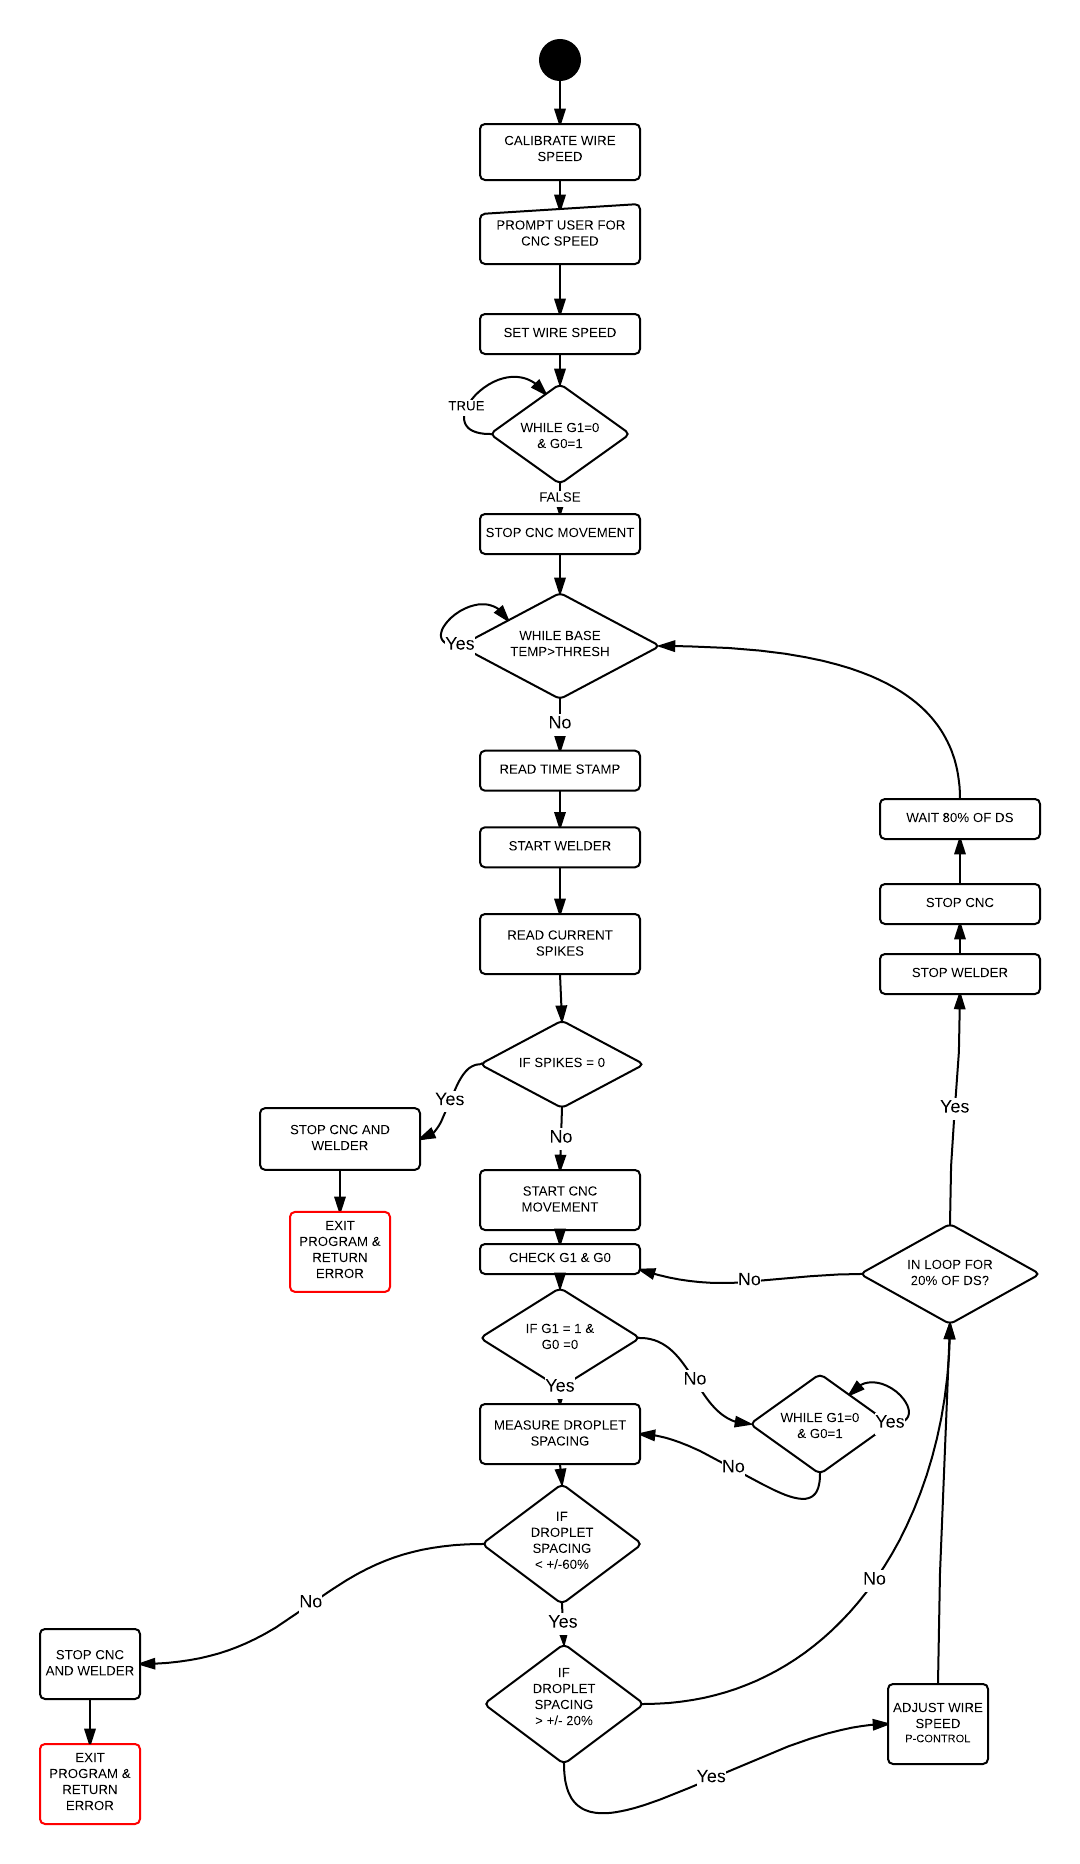
\includegraphics[scale=.7]{control}
\caption{Control Program Flowchart}
\end{figure}



\clearpage


\begin{figure}[!h]
\centering
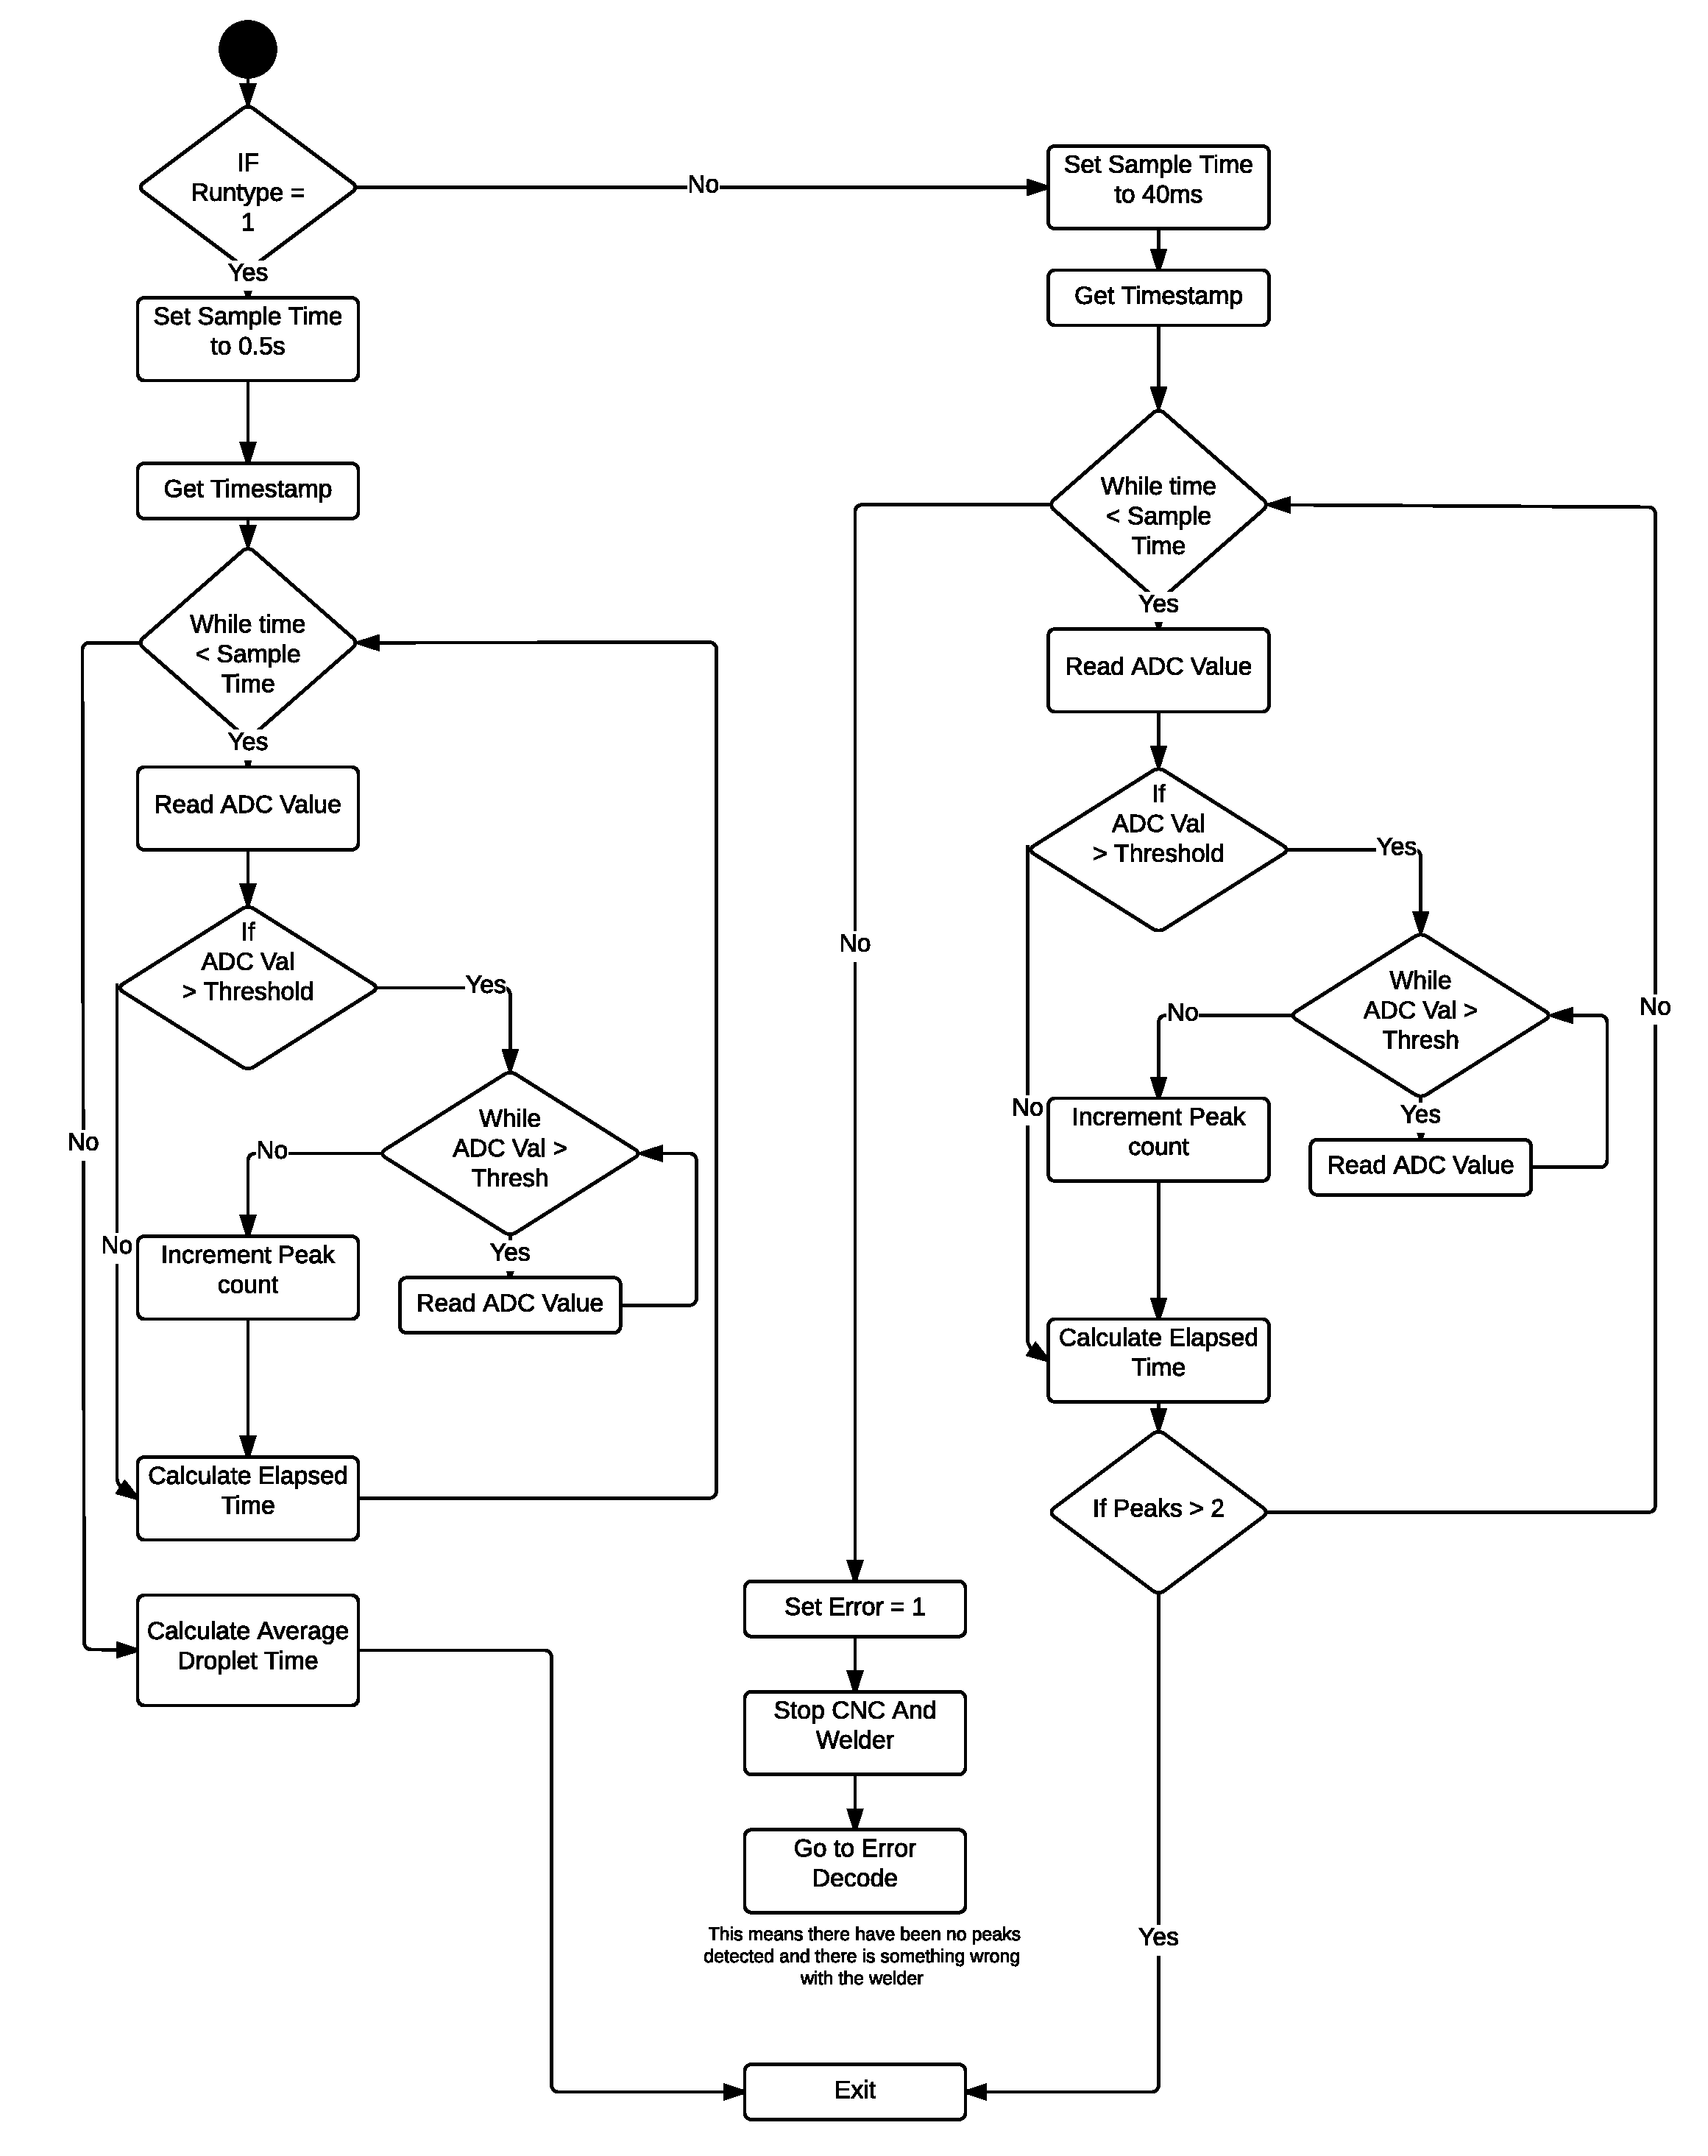
\includegraphics[scale=0.85]{dropletspacing}
\caption{Droplet Spacing Flowchart}
\end{figure}

\clearpage

\begin{figure}[!h]
\centering
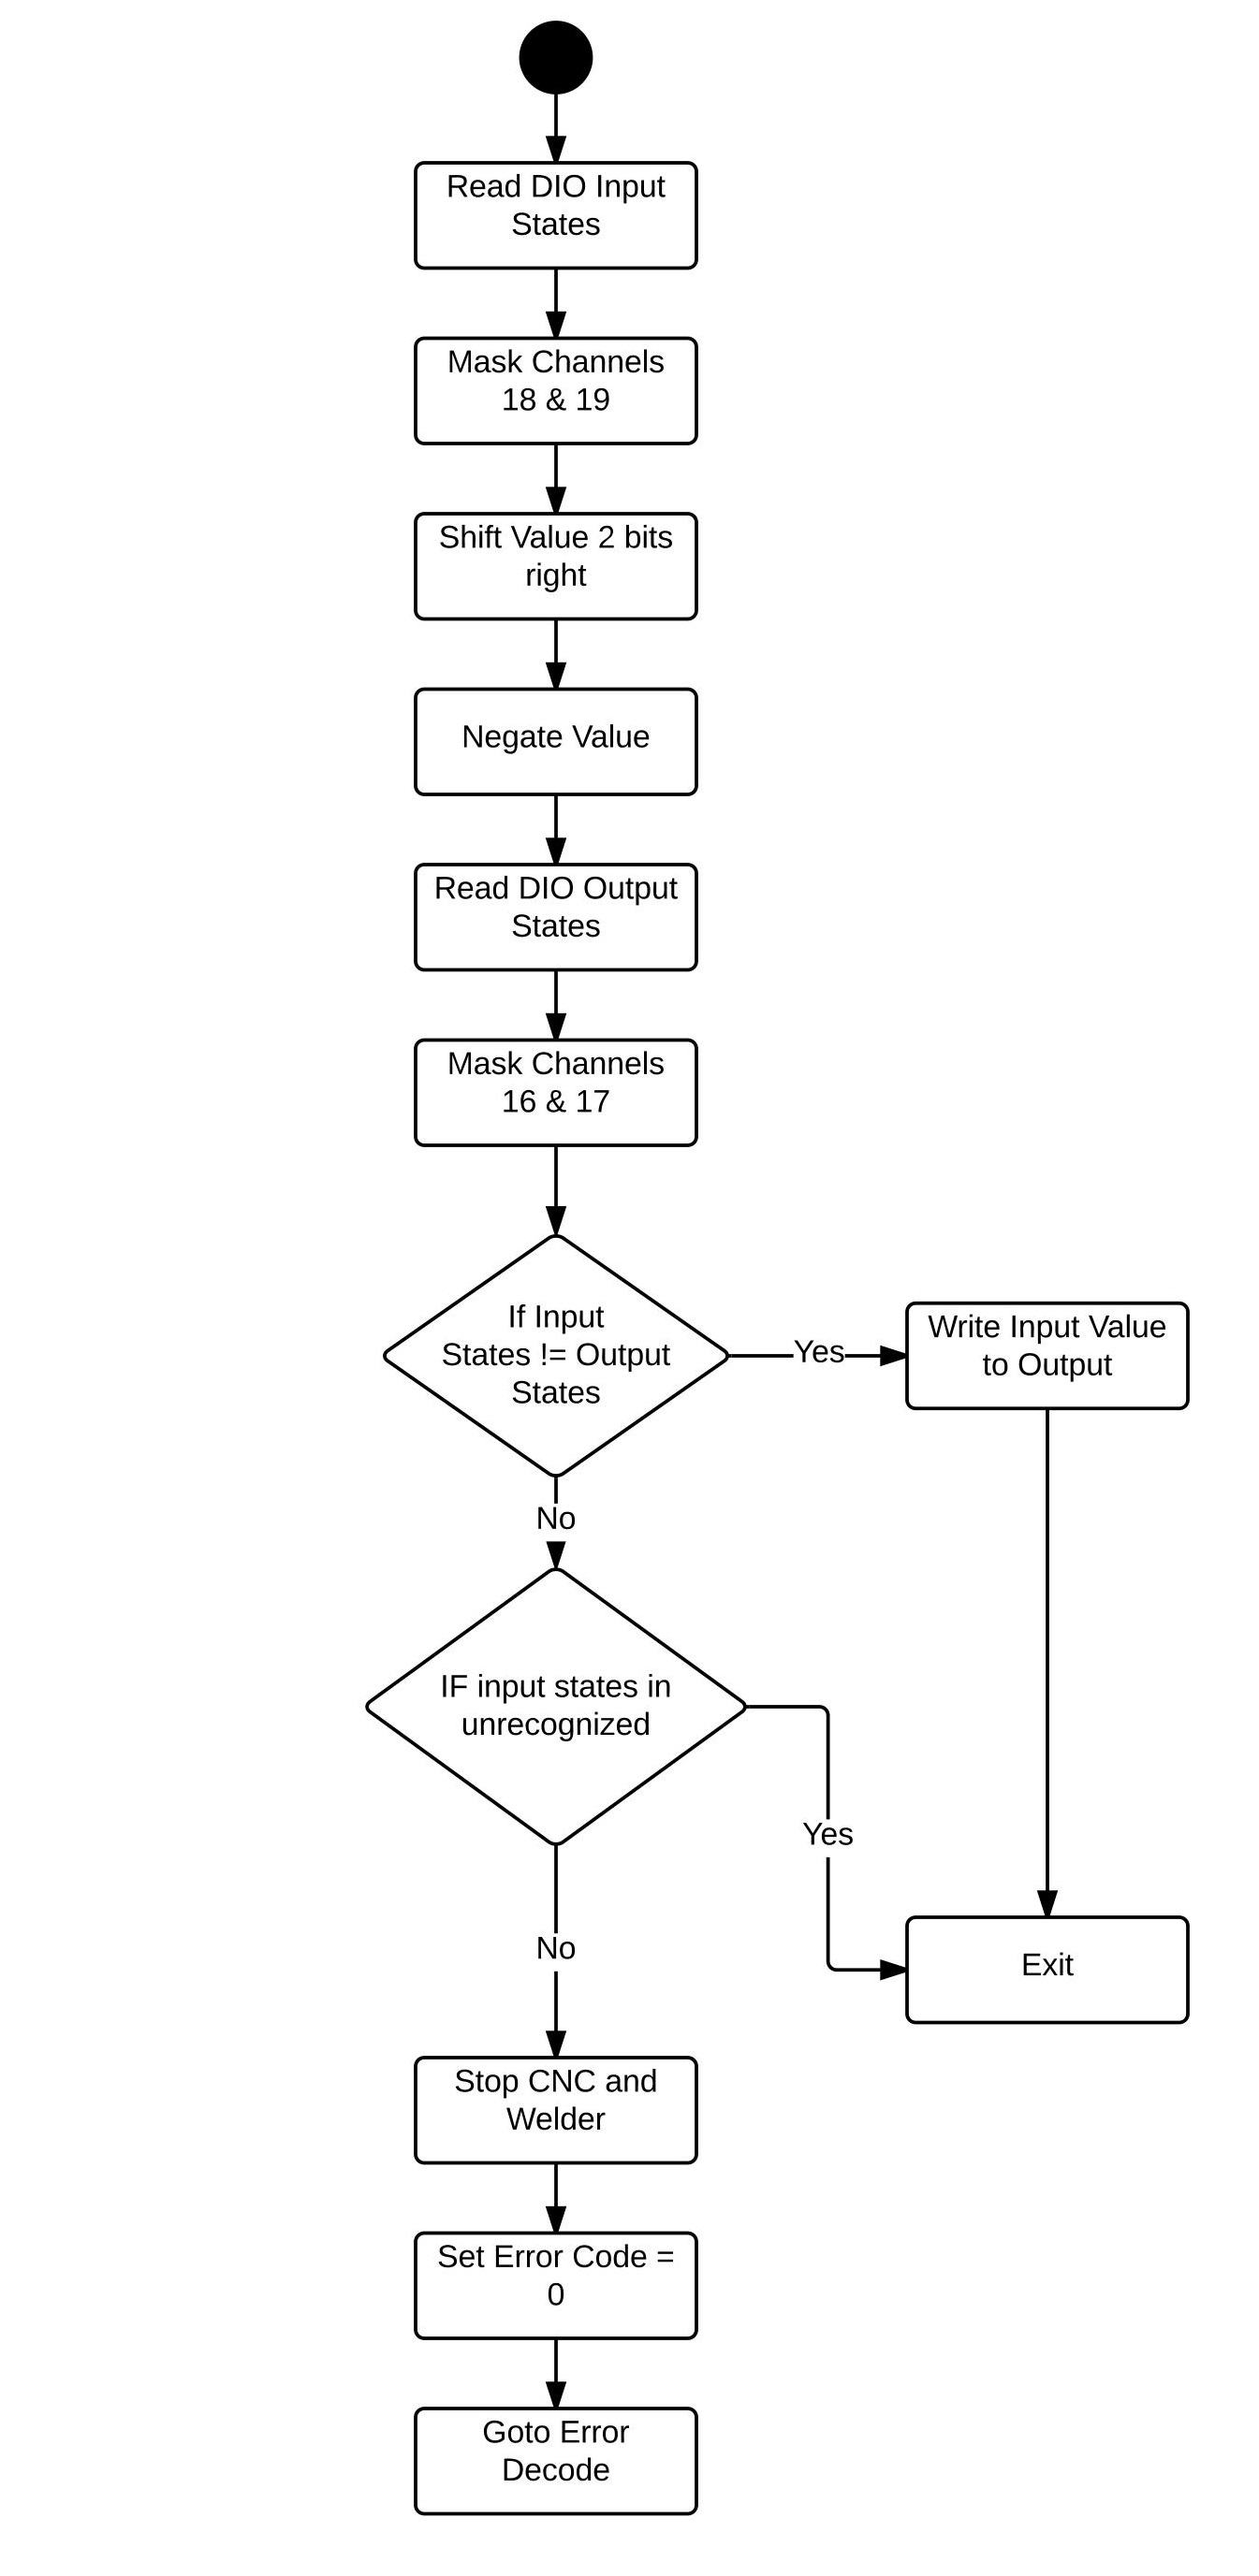
\includegraphics[scale=0.9]{getg0g1}
\caption{Getting G0 \& G1 Flowchart}
\end{figure}

\clearpage


\begin{figure}[!h]
\centering
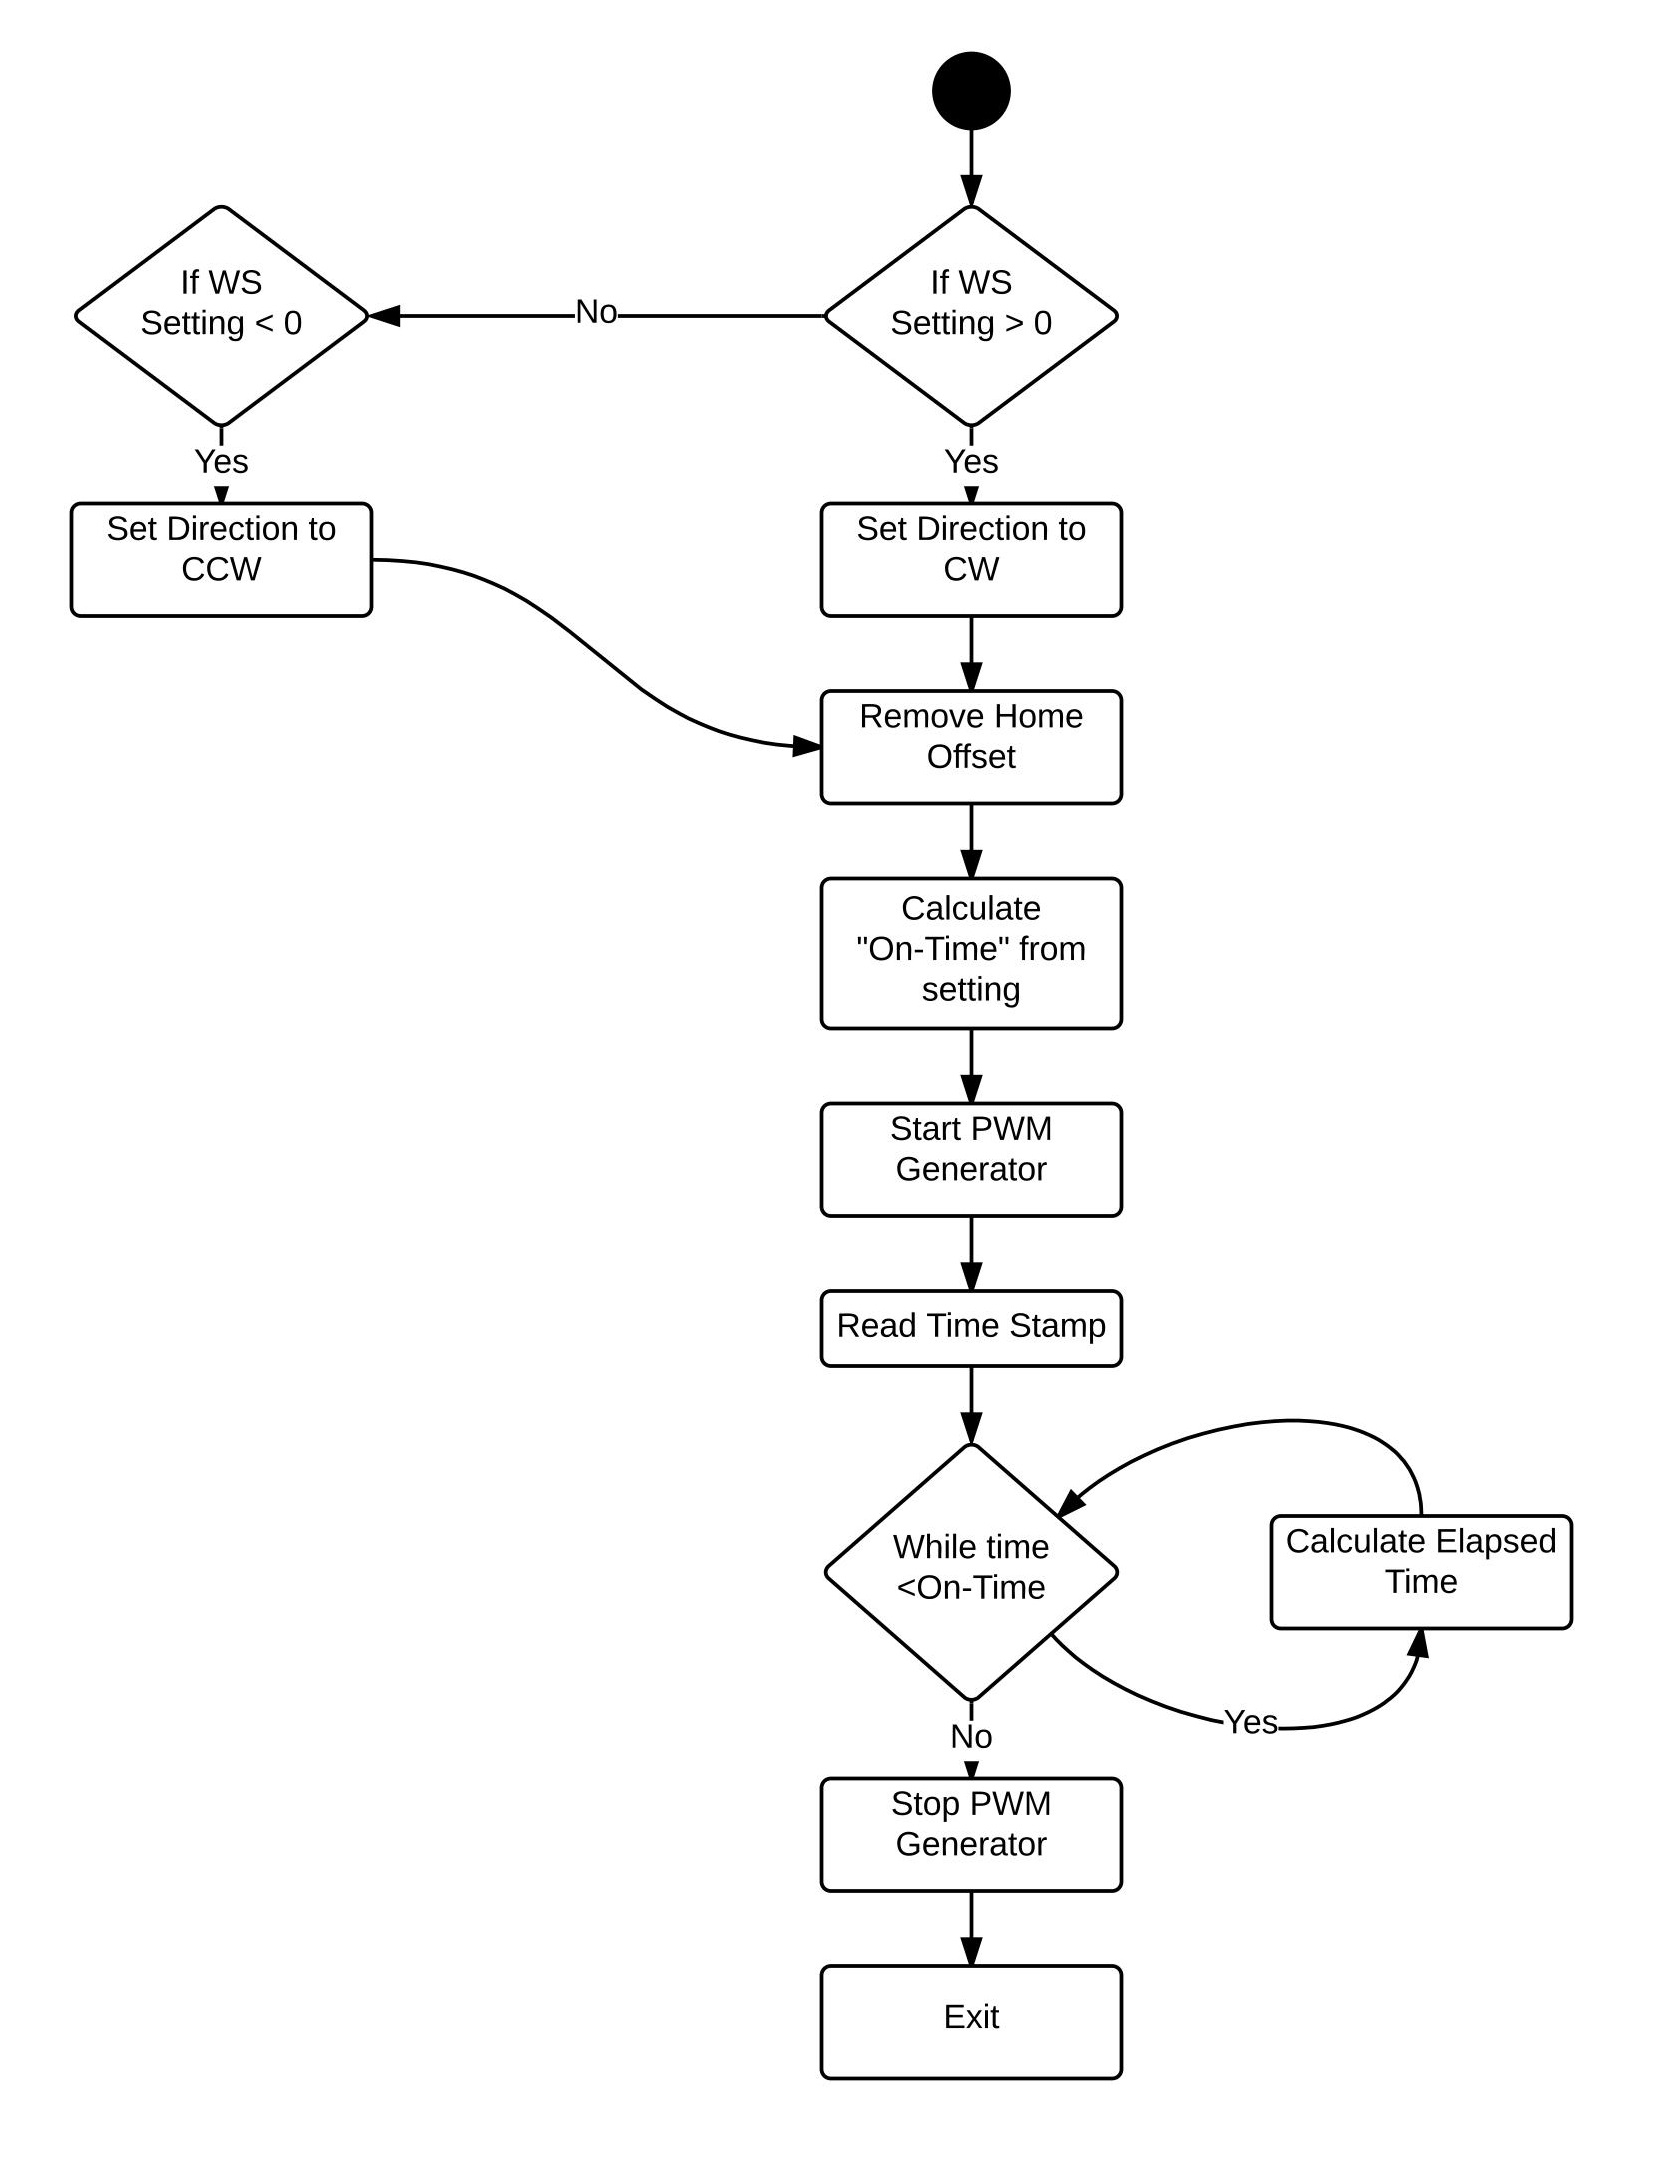
\includegraphics[scale=1.1]{setspeed}
\caption{Set Wire Speed Flowchart}
\end{figure}

\clearpage

\begin{figure}[!h]
\centering
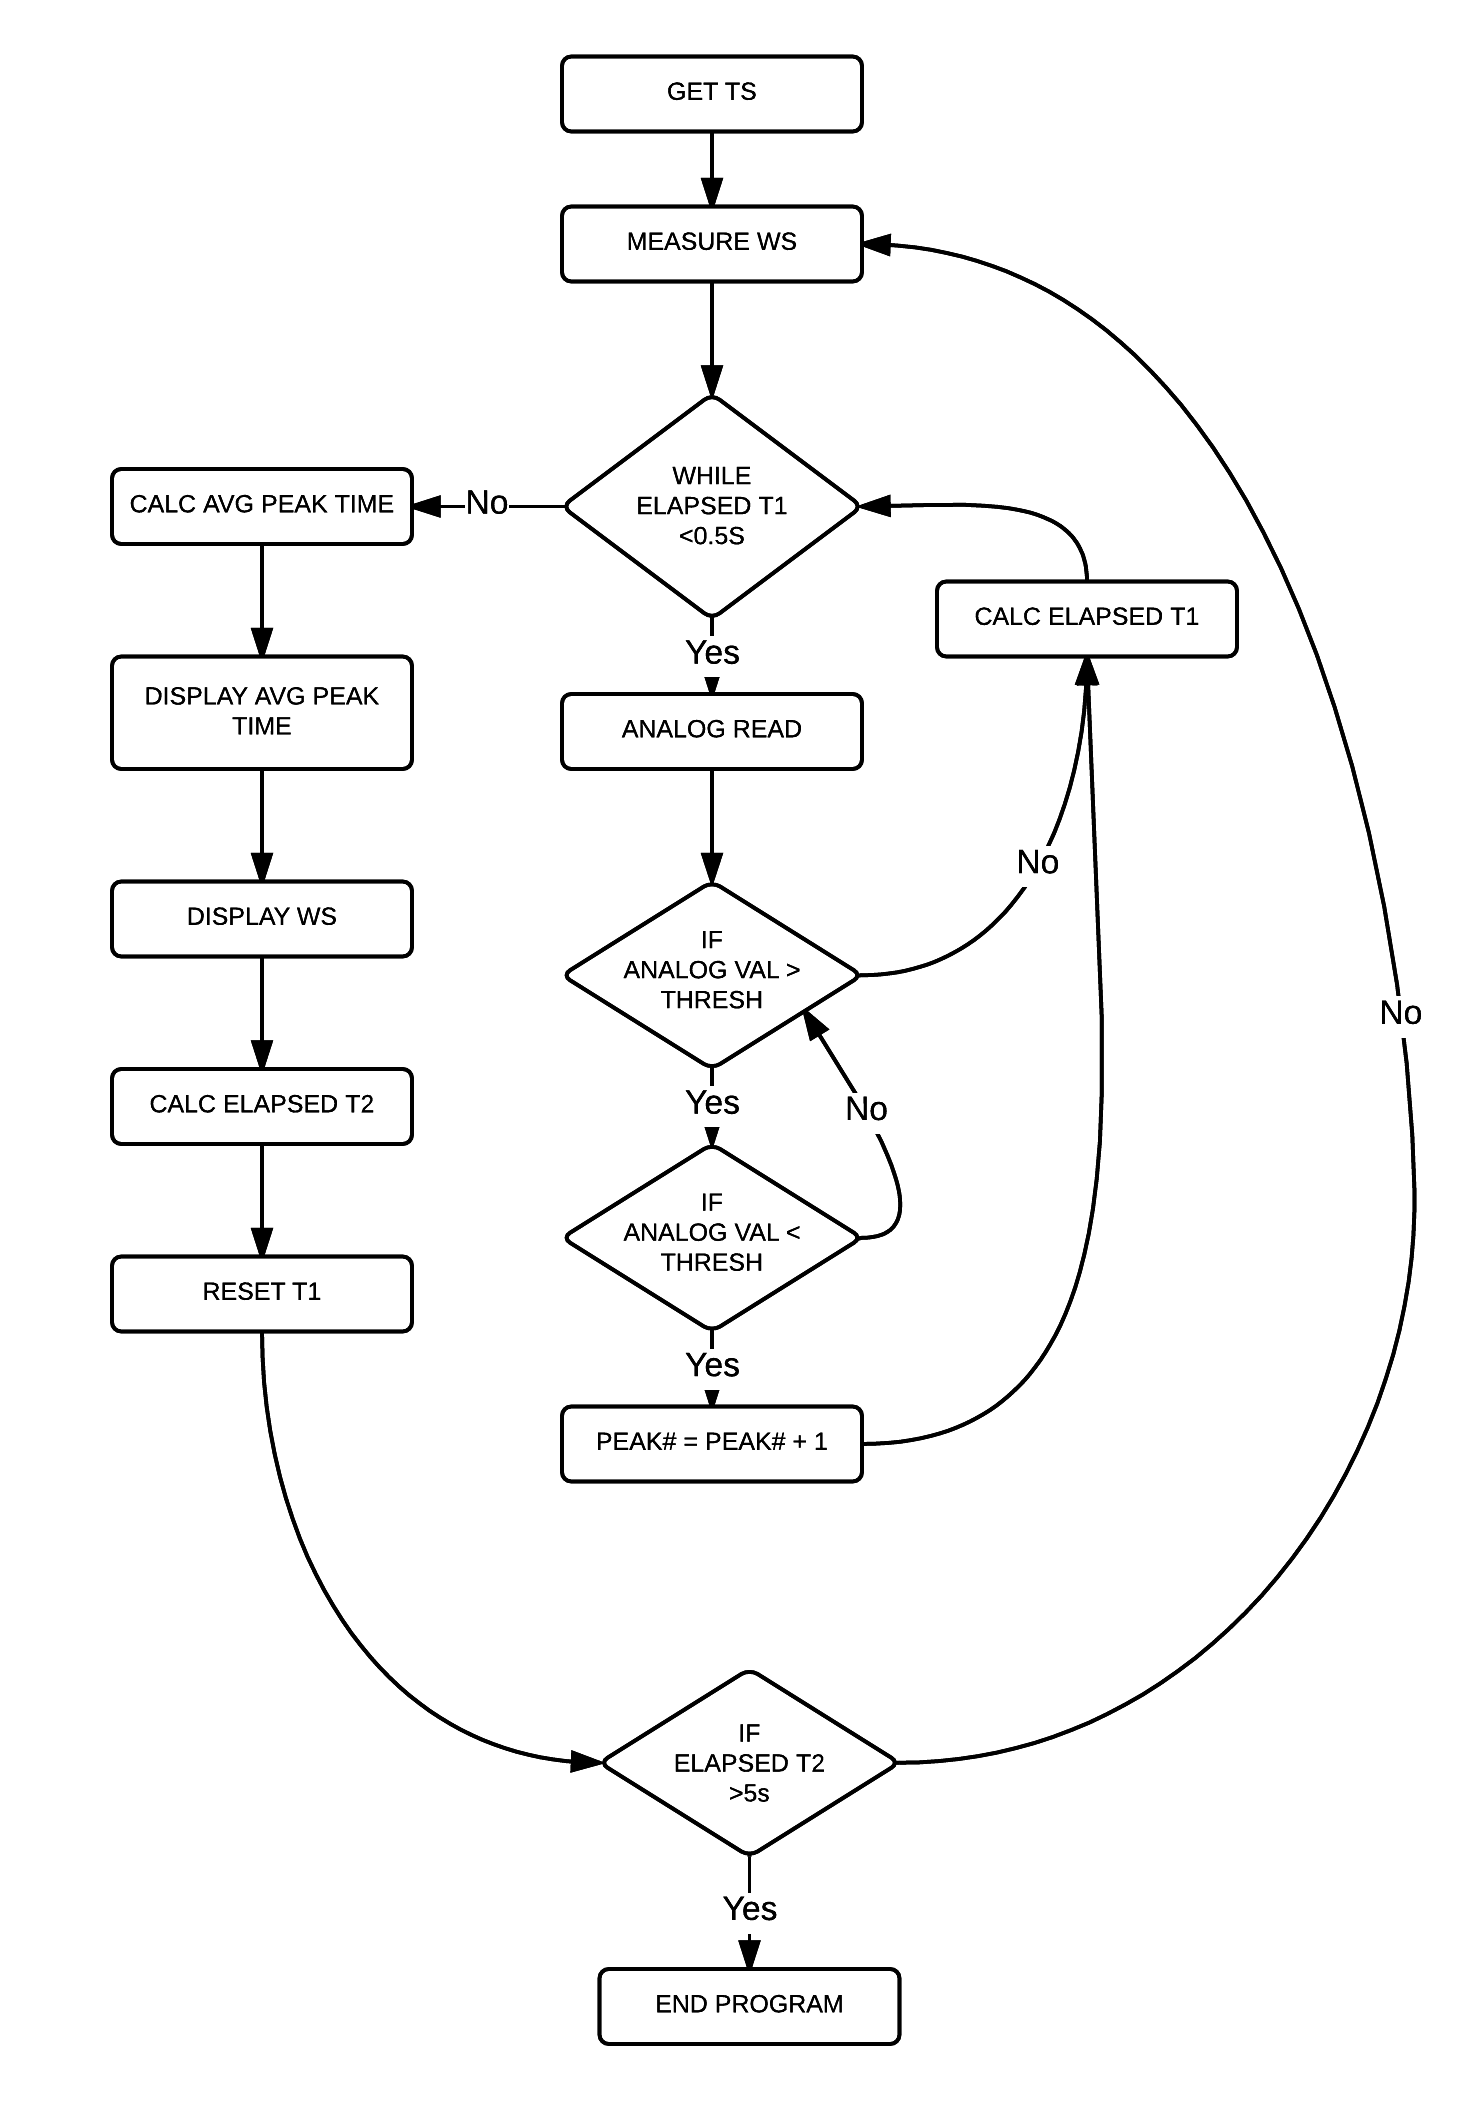
\includegraphics[scale=1.1]{droplet}
\caption{Wire Feed and Droplet Spacing Test Flowchart}
\end{figure}

\clearpage


\subsection{Register Descriptions}




\begin{sidewaystable}[h!]

\begin{center}

%\begin{turn}{90}

\begin{adjustbox}{width=\textwidth}

\begin{tabular}{ cccccccccccccccccccccccccccccccccc }

\cline{1-32}
  
 \multicolumn{1}{|c|}{31} & \multicolumn{1}{c|}{30} & \multicolumn{1}{c|}{29} & \multicolumn{1}{c|}{28} & \multicolumn{1}{c|}{27} & \multicolumn{1}{c|}{26} & \multicolumn{1}{c|}{25} & \multicolumn{1}{c|}{24} & \multicolumn{1}{c|}{23} & \multicolumn{1}{c|}{22} & \multicolumn{1}{c|}{21} & \multicolumn{1}{c|}{20} & \multicolumn{1}{c|}{19} & \multicolumn{1}{c|}{18} & \multicolumn{1}{c|}{17} & \multicolumn{1}{c|}{16} & \multicolumn{1}{c|}{15} & \multicolumn{1}{c|}{14} & \multicolumn{1}{c|}{13} & \multicolumn{1}{c|}{12} & \multicolumn{1}{c|}{11} & \multicolumn{1}{c|}{10} & \multicolumn{1}{c|}{9} & \multicolumn{1}{c|}{8} & \multicolumn{1}{c|}{7} & \multicolumn{1}{c|}{6} & \multicolumn{1}{c|}{5} & \multicolumn{1}{c|}{4} & \multicolumn{1}{c|}{3} & \multicolumn{1}{c|}{2} & \multicolumn{1}{c|}{1} & \multicolumn{1}{c|}{0}   \\ \cline{1-32}
  
 \multicolumn{1}{|c|}{0} & \multicolumn{1}{c|}{IP} & \multicolumn{2}{c|}{IM} & \multicolumn{1}{c|}{0} & \multicolumn{1}{c|}{0} & \multicolumn{1}{c|}{0} & \multicolumn{1}{c|}{TP} & \multicolumn{1}{c|}{NR} & \multicolumn{1}{c|}{UD} & \multicolumn{1}{c|}{BP} & \multicolumn{3}{c|}{OM} & \multicolumn{1}{c|}{OP} & \multicolumn{6}{c|}{TP} & \multicolumn{2}{c|}{TE} & \multicolumn{2}{c|}{TD} & \multicolumn{3}{c|}{K} & \multicolumn{4}{c|}{XS}  \\ \cline{1-32}

\multicolumn{1}{|c}{0} & \multicolumn{1}{|c|}{0} & \multicolumn{1}{c}{0} & \multicolumn{1}{c|}{0} & \multicolumn{1}{c|}{0} & \multicolumn{1}{c|}{0} & \multicolumn{1}{c|}{0} & \multicolumn{1}{c|}{1} & \multicolumn{1}{c|}{0} & \multicolumn{1}{c|}{1} & \multicolumn{1}{c|}{1} & \multicolumn{1}{c}{0} & \multicolumn{1}{c}{1} & \multicolumn{1}{c|}{0} & \multicolumn{1}{c|}{0} & \multicolumn{1}{c}{0} & \multicolumn{1}{c}{0} & \multicolumn{1}{c}{0} & \multicolumn{1}{c}{1} & \multicolumn{1}{c}{0} & \multicolumn{1}{c|}{0} & \multicolumn{1}{c}{0} & \multicolumn{1}{c|}{0} & \multicolumn{1}{c}{0} & \multicolumn{1}{c|}{} & \multicolumn{1}{c}{0} & \multicolumn{1}{c}{1} & \multicolumn{1}{c|}{0} & \multicolumn{1}{c}{0} & \multicolumn{1}{c}{0} & \multicolumn{1}{c}{0} & \multicolumn{1}{c|}{0}   \\ \cline{1-32}

\multicolumn{4}{|c|}{0} & \multicolumn{4}{c|}{1} & \multicolumn{4}{c|}{6} & \multicolumn{4}{c|}{8} & \multicolumn{4}{c|}{2} & \multicolumn{4}{c|}{0} & \multicolumn{4}{c|}{2} & \multicolumn{4}{c|}{0}  \\ \cline{1-32}

& & & & & & & & & & & & & & & & & & & & & & & & & & & & & & &  \\ \cline{1-32}

\multicolumn{1}{|c}{0} & \multicolumn{1}{|c|}{0} & \multicolumn{1}{c}{0} & \multicolumn{1}{c|}{0} & \multicolumn{1}{c|}{0} & \multicolumn{1}{c|}{0} & \multicolumn{1}{c|}{0} & \multicolumn{1}{c|}{0} & \multicolumn{1}{c|}{0} & \multicolumn{1}{c|}{0} & \multicolumn{1}{c|}{0} & \multicolumn{1}{c}{0} & \multicolumn{1}{c}{0} & \multicolumn{1}{c|}{0} & \multicolumn{1}{c|}{0} & \multicolumn{1}{c}{0} & \multicolumn{1}{c}{1} & \multicolumn{1}{c}{0} & \multicolumn{1}{c}{0} & \multicolumn{1}{c}{0} & \multicolumn{1}{c|}{0} & \multicolumn{1}{c}{0} & \multicolumn{1}{c|}{0} & \multicolumn{1}{c}{0} & \multicolumn{1}{c|}{0} & \multicolumn{1}{c}{0} & \multicolumn{1}{c}{0} & \multicolumn{1}{c|}{0} & \multicolumn{1}{c}{1} & \multicolumn{1}{c}{0} & \multicolumn{1}{c}{1} & \multicolumn{1}{c|}{0}   \\ \cline{1-32}

\multicolumn{4}{|c|}{0} & \multicolumn{4}{c|}{0} & \multicolumn{4}{c|}{0} & \multicolumn{4}{c|}{0} & \multicolumn{4}{c|}{8} & \multicolumn{4}{c|}{0} & \multicolumn{4}{c|}{0} & \multicolumn{4}{c|}{A}  \\ \cline{1-32}

 
\end{tabular}
\end{adjustbox}
%\end{turn}

\captionof{table}{Counter Mode Register Description} 
\label{countermode}
\end{center}

\end{sidewaystable}

The following list shows the definitions for the rows in Table \ref{countermode}:

\begin{itemize*}
	\item Row 3 - BIN VAL For PWM Mode
	\item Row 4 - HEX VAL
	\item Row 5 - BIN VAL For Frequency Measurement Mode
	\item Row 6 - HEX VAL
\end{itemize*}




\begin{sidewaystable}[h!]

\begin{center}

\begin{adjustbox}{width=\textwidth}

\begin{tabu}{ |c|c|c|c|c|c|c|c|c|c|c|c|c|c|c|c|c|c|c|c|c|c|c|c|c|c|c|c|c|c|c|c| }

\cline{1-32}
  
  \multicolumn{1}{|c|}{31} & 30 & 29 & 28 & 27 & 26 & 25 & 24 & 23 & 22 & 21 & 20 & 19 & 18 & 17 & 16 & 15 & 14 & 13 & 12 & 11 & 10 & 9 & 8 & 7 & 6 & 5 & 4 & 3 & 2 & 1 & 0  \\ \cline{1-32}
  
  \multicolumn{1}{|c|}{-} & - & - & - & - & - & - & - & 23 & 22 & 21 & 20 & 19 & 18 & 17 & 16 & 15 & 14 & 13 & 12 & 11 & 10 & 9 & 8 & 7 & 6 & 5 & 4 & 3 & 2 & 1 & 0  \\ \cline{1-32}
  
  \multicolumn{1}{|c|}{-} & - & - & - & - & - & - & - & 1 & 3 & 5 & 7 & 9 & 11 & 13 & 15 & 17 & 19 & 21 & 23 & 25 & 27 & 29 & 31 & 33 & 35 & 37 & 39 & 41 & 43 & 45 & 47  \\ \tabucline[1pt]{9-32} \cline{1-8}
  
  \multicolumn{1}{c}{} & \multicolumn{1}{c}{} & \multicolumn{1}{c}{} & \multicolumn{1}{c}{} & \multicolumn{1}{c}{} & \multicolumn{1}{c}{} & \multicolumn{1}{c}{} & \multicolumn{1}{c}{} & 1 & 3 & 5 & 7 & 9 & 11 & 13 & 15 & 17 & 19 & 21 & 23 & 25 & 27 & 29 & 31 & 33 & 35 & 37 & 39 & 41 & 43 & 45 & 47  \\ \tabucline[1pt]{9-32} \cline{9-32}
  
  
  
  \multicolumn{1}{c}{} & \multicolumn{1}{c}{} & \multicolumn{1}{c}{} & \multicolumn{1}{c}{} & \multicolumn{1}{c}{} & \multicolumn{1}{c}{} & \multicolumn{1}{c}{} & \multicolumn{1}{c}{} & \multicolumn{1}{|[2pt]c|}{\cellcolor{red!25}$\times$} & \multicolumn{1}{c|}{\cellcolor{red!25}$\times$} & \multicolumn{1}{c}{\cellcolor{red!25}$\times$} & \multicolumn{1}{|c}{\cellcolor{red!25}$\times$} & \multicolumn{1}{|[1pt]c|}{\cellcolor{red!25}$\times$} & \multicolumn{1}{c|}{\cellcolor{red!25}$\times$} & \multicolumn{1}{c|}{\cellcolor{green!25}1} & \multicolumn{1}{c|}{\cellcolor{green!25}1} & \multicolumn{1}{|[1pt]c|}{\cellcolor{red!25}$\times$} & \multicolumn{1}{c}{\cellcolor{red!25}$\times$} & \multicolumn{1}{|c|}{\cellcolor{red!25}$\times$} & \multicolumn{1}{|c}{\cellcolor{red!25}$\times$} & \multicolumn{1}{|[1pt]c|}{\cellcolor{red!25}$\times$} & \multicolumn{1}{|c|}{\cellcolor{red!25}$\times$} & \multicolumn{1}{|c}{\cellcolor{red!25}$\times$} & \multicolumn{1}{|c|}{\cellcolor{red!25}$\times$} & \multicolumn{1}{|[1pt]c}{\cellcolor{red!25}$\times$} & \multicolumn{1}{|c}{\cellcolor{red!25}$\times$} & \multicolumn{1}{|c}{\cellcolor{red!25}$\times$} & \multicolumn{1}{|c}{\cellcolor{red!25}$\times$} & \multicolumn{1}{|[1pt]c|}{\cellcolor{red!25}$\times$} & \multicolumn{1}{c|}{\cellcolor{red!25}$\times$} & \multicolumn{1}{c|}{\cellcolor{red!25}$\times$} & \multicolumn{1}{c|[2pt]}{\cellcolor{red!25}$\times$}   \\ \tabucline[1pt]{9-32}
  
  
  \multicolumn{1}{c}{} & \multicolumn{1}{c}{} & \multicolumn{1}{c}{} & \multicolumn{1}{c}{} & \multicolumn{1}{c}{} & \multicolumn{1}{c}{} & \multicolumn{1}{c}{} & \multicolumn{1}{c}{} & \multicolumn{1}{|[2pt]c|}{\cellcolor{red!25}$\times$} & \multicolumn{1}{c|}{\cellcolor{red!25}$\times$} & \multicolumn{1}{c}{\cellcolor{red!25}$\times$} & \multicolumn{1}{|c}{\cellcolor{red!25}$\times$} & \multicolumn{1}{|[1pt]c|}{\cellcolor{green!25}0} & \multicolumn{1}{c|}{\cellcolor{green!25}1} & \multicolumn{1}{c|}{\cellcolor{red!25}$\times$} & \multicolumn{1}{c|}{\cellcolor{red!25}$\times$} & \multicolumn{1}{|[1pt]c|}{\cellcolor{red!25}$\times$} & \multicolumn{1}{c}{\cellcolor{red!25}$\times$} & \multicolumn{1}{|c|}{\cellcolor{red!25}$\times$} & \multicolumn{1}{|c}{\cellcolor{red!25}$\times$} & \multicolumn{1}{|[1pt]c|}{\cellcolor{red!25}$\times$} & \multicolumn{1}{|c|}{\cellcolor{red!25}$\times$} & \multicolumn{1}{|c}{\cellcolor{red!25}$\times$} & \multicolumn{1}{|c|}{\cellcolor{red!25}$\times$} & \multicolumn{1}{|[1pt]c}{\cellcolor{red!25}$\times$} & \multicolumn{1}{|c}{\cellcolor{red!25}$\times$} & \multicolumn{1}{|c}{\cellcolor{red!25}$\times$} & \multicolumn{1}{|c}{\cellcolor{red!25}$\times$} & \multicolumn{1}{|[1pt]c|}{\cellcolor{red!25}$\times$} & \multicolumn{1}{c|}{\cellcolor{red!25}$\times$} & \multicolumn{1}{c|}{\cellcolor{red!25}$\times$} & \multicolumn{1}{c|[2pt]}{\cellcolor{red!25}$\times$}   \\ \tabucline[2pt]{9-32}


\multicolumn{1}{c}{} & \multicolumn{1}{c}{} & \multicolumn{1}{c}{} & \multicolumn{1}{c}{} & \multicolumn{1}{c}{} & \multicolumn{1}{c}{} & \multicolumn{1}{c}{} & \multicolumn{1}{c}{} & \multicolumn{1}{|[2pt]c|}{\cellcolor{red!25}$\times$} & \multicolumn{1}{c|}{\cellcolor{red!25}$\times$} & \multicolumn{1}{c}{\cellcolor{red!25}$\times$} & \multicolumn{1}{|c}{\cellcolor{red!25}$\times$} & \multicolumn{1}{|[1pt]c|}{\cellcolor{green!25}1} & \multicolumn{1}{c|}{\cellcolor{green!25}0} & \multicolumn{1}{c|}{\cellcolor{red!25}$\times$} & \multicolumn{1}{c|}{\cellcolor{red!25}$\times$} & \multicolumn{1}{|[1pt]c|}{\cellcolor{red!25}$\times$} & \multicolumn{1}{c}{\cellcolor{red!25}$\times$} & \multicolumn{1}{|c|}{\cellcolor{red!25}$\times$} & \multicolumn{1}{|c}{\cellcolor{red!25}$\times$} & \multicolumn{1}{|[1pt]c|}{\cellcolor{red!25}$\times$} & \multicolumn{1}{|c|}{\cellcolor{red!25}$\times$} & \multicolumn{1}{|c}{\cellcolor{red!25}$\times$} & \multicolumn{1}{|c|}{\cellcolor{red!25}$\times$} & \multicolumn{1}{|[1pt]c}{\cellcolor{red!25}$\times$} & \multicolumn{1}{|c}{\cellcolor{red!25}$\times$} & \multicolumn{1}{|c}{\cellcolor{red!25}$\times$} & \multicolumn{1}{|c}{\cellcolor{red!25}$\times$} & \multicolumn{1}{|[1pt]c|}{\cellcolor{red!25}$\times$} & \multicolumn{1}{c|}{\cellcolor{red!25}$\times$} & \multicolumn{1}{c|}{\cellcolor{red!25}$\times$} & \multicolumn{1}{c|[2pt]}{\cellcolor{red!25}$\times$}   \\ \tabucline[2pt]{9-32}


\multicolumn{1}{c}{} & \multicolumn{1}{c}{} & \multicolumn{1}{c}{} & \multicolumn{1}{c}{} & \multicolumn{1}{c}{} & \multicolumn{1}{c}{} & \multicolumn{1}{c}{} & \multicolumn{1}{c}{} & \multicolumn{1}{|[2pt]c|}{\cellcolor{red!25}$\times$} & \multicolumn{1}{c|}{\cellcolor{green!25}1} & \multicolumn{1}{c}{\cellcolor{red!25}$\times$} & \multicolumn{1}{|c}{\cellcolor{red!25}$\times$} & \multicolumn{1}{|[1pt]c|}{\cellcolor{red!25}$\times$} & \multicolumn{1}{c|}{\cellcolor{red!25}$\times$} & \multicolumn{1}{c|}{\cellcolor{red!25}$\times$} & \multicolumn{1}{c|}{\cellcolor{red!25}$\times$} & \multicolumn{1}{|[1pt]c|}{\cellcolor{red!25}$\times$} & \multicolumn{1}{c}{\cellcolor{red!25}$\times$} & \multicolumn{1}{|c|}{\cellcolor{red!25}$\times$} & \multicolumn{1}{|c}{\cellcolor{red!25}$\times$} & \multicolumn{1}{|[1pt]c|}{\cellcolor{red!25}$\times$} & \multicolumn{1}{|c|}{\cellcolor{red!25}$\times$} & \multicolumn{1}{|c|}{\cellcolor{red!25}$\times$} & \multicolumn{1}{|c}{\cellcolor{red!25}$\times$} & \multicolumn{1}{|[1pt]c}{\cellcolor{red!25}$\times$} & \multicolumn{1}{|c}{\cellcolor{red!25}$\times$} & \multicolumn{1}{|c}{\cellcolor{red!25}$\times$} & \multicolumn{1}{|c}{\cellcolor{red!25}$\times$} & \multicolumn{1}{|[1pt]c|}{\cellcolor{red!25}$\times$} & \multicolumn{1}{c|}{\cellcolor{red!25}$\times$} & \multicolumn{1}{c|}{\cellcolor{red!25}$\times$} & \multicolumn{1}{c|[2pt]}{\cellcolor{red!25}$\times$}   \\ \tabucline[2pt]{9-32}


\multicolumn{1}{c}{} & \multicolumn{1}{c}{} & \multicolumn{1}{c}{} & \multicolumn{1}{c}{} & \multicolumn{1}{c}{} & \multicolumn{1}{c}{} & \multicolumn{1}{c}{} & \multicolumn{1}{c}{} & \multicolumn{1}{|[2pt]c|}{\cellcolor{red!25}$\times$} & \multicolumn{1}{c|}{\cellcolor{green!25}0} & \multicolumn{1}{c}{\cellcolor{red!25}$\times$} & \multicolumn{1}{|c}{\cellcolor{red!25}$\times$} & \multicolumn{1}{|[1pt]c|}{\cellcolor{red!25}$\times$} & \multicolumn{1}{c|}{\cellcolor{red!25}$\times$} & \multicolumn{1}{c|}{\cellcolor{red!25}$\times$} & \multicolumn{1}{c|}{\cellcolor{red!25}$\times$} & \multicolumn{1}{|[1pt]c|}{\cellcolor{red!25}$\times$} & \multicolumn{1}{c}{\cellcolor{red!25}$\times$} & \multicolumn{1}{|c|}{\cellcolor{red!25}$\times$} & \multicolumn{1}{|c}{\cellcolor{red!25}$\times$} & \multicolumn{1}{|[1pt]c|}{\cellcolor{red!25}$\times$} & \multicolumn{1}{|c|}{\cellcolor{red!25}$\times$} & \multicolumn{1}{|c|}{\cellcolor{red!25}$\times$} & \multicolumn{1}{|c}{\cellcolor{red!25}$\times$} & \multicolumn{1}{|[1pt]c}{\cellcolor{red!25}$\times$} & \multicolumn{1}{|c}{\cellcolor{red!25}$\times$} & \multicolumn{1}{|c}{\cellcolor{red!25}$\times$} & \multicolumn{1}{|c}{\cellcolor{red!25}$\times$} & \multicolumn{1}{|[1pt]c|}{\cellcolor{red!25}$\times$} & \multicolumn{1}{c|}{\cellcolor{red!25}$\times$} & \multicolumn{1}{c|}{\cellcolor{red!25}$\times$} & \multicolumn{1}{c|[2pt]}{\cellcolor{red!25}$\times$}   \\ \tabucline[2pt]{9-32}


\multicolumn{1}{c}{} & \multicolumn{1}{c}{} & \multicolumn{1}{c}{} & \multicolumn{1}{c}{} & \multicolumn{1}{c}{} & \multicolumn{1}{c}{} & \multicolumn{1}{c}{} & \multicolumn{1}{c}{} & \multicolumn{1}{|[2pt]c|}{\cellcolor{red!25}$\times$} & \multicolumn{1}{c|}{\cellcolor{red!25}$\times$} & \multicolumn{1}{c}{\cellcolor{green!25}0} & \multicolumn{1}{|c}{\cellcolor{red!25}$\times$} & \multicolumn{1}{|[1pt]c|}{\cellcolor{red!25}$\times$} & \multicolumn{1}{c|}{\cellcolor{red!25}$\times$} & \multicolumn{1}{c|}{\cellcolor{red!25}$\times$} & \multicolumn{1}{c|}{\cellcolor{red!25}$\times$} & \multicolumn{1}{|[1pt]c|}{\cellcolor{red!25}$\times$} & \multicolumn{1}{c}{\cellcolor{red!25}$\times$} & \multicolumn{1}{|c|}{\cellcolor{red!25}$\times$} & \multicolumn{1}{|c}{\cellcolor{red!25}$\times$} & \multicolumn{1}{|[1pt]c|}{\cellcolor{red!25}$\times$} & \multicolumn{1}{|c|}{\cellcolor{red!25}$\times$} & \multicolumn{1}{|c|}{\cellcolor{red!25}$\times$} & \multicolumn{1}{|c}{\cellcolor{red!25}$\times$} & \multicolumn{1}{|[1pt]c}{\cellcolor{red!25}$\times$} & \multicolumn{1}{|c}{\cellcolor{red!25}$\times$} & \multicolumn{1}{|c}{\cellcolor{red!25}$\times$} & \multicolumn{1}{|c}{\cellcolor{red!25}$\times$} & \multicolumn{1}{|[1pt]c|}{\cellcolor{red!25}$\times$} & \multicolumn{1}{c|}{\cellcolor{red!25}$\times$} & \multicolumn{1}{c|}{\cellcolor{red!25}$\times$} & \multicolumn{1}{c|[2pt]}{\cellcolor{red!25}$\times$}   \\ \tabucline[2pt]{9-32}


\multicolumn{1}{c}{} & \multicolumn{1}{c}{} & \multicolumn{1}{c}{} & \multicolumn{1}{c}{} & \multicolumn{1}{c}{} & \multicolumn{1}{c}{} & \multicolumn{1}{c}{} & \multicolumn{1}{c}{} & \multicolumn{1}{|[2pt]c|}{\cellcolor{green!25}1} & \multicolumn{1}{c|}{\cellcolor{red!25}$\times$} & \multicolumn{1}{c}{\cellcolor{red!25}$\times$} & \multicolumn{1}{|c}{\cellcolor{red!25}$\times$} & \multicolumn{1}{|[1pt]c|}{\cellcolor{red!25}$\times$} & \multicolumn{1}{c|}{\cellcolor{red!25}$\times$} & \multicolumn{1}{c|}{\cellcolor{green!25}1} & \multicolumn{1}{c|}{\cellcolor{green!25}1} & \multicolumn{1}{|[1pt]c|}{\cellcolor{red!25}$\times$} & \multicolumn{1}{c}{\cellcolor{red!25}$\times$} & \multicolumn{1}{|c|}{\cellcolor{red!25}$\times$} & \multicolumn{1}{|c}{\cellcolor{red!25}$\times$} & \multicolumn{1}{|[1pt]c|}{\cellcolor{red!25}$\times$} & \multicolumn{1}{|c|}{\cellcolor{red!25}$\times$} & \multicolumn{1}{|c|}{\cellcolor{red!25}$\times$} & \multicolumn{1}{|c}{\cellcolor{red!25}$\times$} & \multicolumn{1}{|[1pt]c}{\cellcolor{red!25}$\times$} & \multicolumn{1}{|c}{\cellcolor{red!25}$\times$} & \multicolumn{1}{|c}{\cellcolor{red!25}$\times$} & \multicolumn{1}{|c}{\cellcolor{red!25}$\times$} & \multicolumn{1}{|[1pt]c|}{\cellcolor{red!25}$\times$} & \multicolumn{1}{c|}{\cellcolor{red!25}$\times$} & \multicolumn{1}{c|}{\cellcolor{red!25}$\times$} & \multicolumn{1}{c|[2pt]}{\cellcolor{red!25}$\times$}   \\ \tabucline[2pt]{9-32}


\multicolumn{1}{c}{} & \multicolumn{1}{c}{} & \multicolumn{1}{c}{} & \multicolumn{1}{c}{} & \multicolumn{1}{c}{} & \multicolumn{1}{c}{} & \multicolumn{1}{c}{} & \multicolumn{1}{c}{} & \multicolumn{1}{|[2pt]c|}{\cellcolor{red!25}$\times$} & \multicolumn{1}{c|}{\cellcolor{red!25}$\times$} & \multicolumn{1}{c}{\cellcolor{red!25}$\times$} & \multicolumn{1}{|c}{\cellcolor{red!25}$\times$} & \multicolumn{1}{|[1pt]c|}{\cellcolor{green!25}1} & \multicolumn{1}{c|}{\cellcolor{green!25}0} & \multicolumn{1}{c|}{\cellcolor{red!25}$\times$} & \multicolumn{1}{c|}{\cellcolor{red!25}$\times$} & \multicolumn{1}{|[1pt]c|}{\cellcolor{red!25}$\times$} & \multicolumn{1}{c}{\cellcolor{red!25}$\times$} & \multicolumn{1}{|c|}{\cellcolor{red!25}$\times$} & \multicolumn{1}{|c}{\cellcolor{red!25}$\times$} & \multicolumn{1}{|[1pt]c|}{\cellcolor{red!25}$\times$} & \multicolumn{1}{|c|}{\cellcolor{red!25}$\times$} & \multicolumn{1}{|c|}{\cellcolor{red!25}$\times$} & \multicolumn{1}{|c}{\cellcolor{red!25}$\times$} & \multicolumn{1}{|[1pt]c}{\cellcolor{red!25}$\times$} & \multicolumn{1}{|c}{\cellcolor{red!25}$\times$} & \multicolumn{1}{|c}{\cellcolor{red!25}$\times$} & \multicolumn{1}{|c}{\cellcolor{red!25}$\times$} & \multicolumn{1}{|[1pt]c|}{\cellcolor{red!25}$\times$} & \multicolumn{1}{c|}{\cellcolor{red!25}$\times$} & \multicolumn{1}{c|}{\cellcolor{red!25}$\times$} & \multicolumn{1}{c|[2pt]}{\cellcolor{red!25}$\times$}   \\ \tabucline[2pt]{9-32}

\end{tabu}
\end{adjustbox}

\captionof{table}{DIO[0] Register Description} 
\label{dioref}
\end{center}

\end{sidewaystable}

The following list shows the definitions for the rows in Table \ref{dioref}:

\begin{itemize*}
		\item Row 1 - Bit
		\item Row 2 - Channel
		\item Row 3 - Pin
		\item Row 4 - G1/G0 Read Mask
		\item Row 5 - G1/G0 Write Mask
		\item Row 6 - G1 INPUT ACTIVE
		\item Row 7 - G0 INPUT ACTIVE
		\item Row 8 - Motor CCW
		\item Row 9 - Motor CW
		\item Row 10 - Wire Speed Home Switch
		\item Row 11 - Weld and CNC stop
		\item Row 12 - CNC start
\end{itemize*}

\clearpage



\subsection{GUI Description}

The initial plan was to have a GUI for our software and but was later not pursued due to time constraints. In GUI the user could see real-time graphed data coming from the current and temperature sensors as well as see the current wire speed. The system would use this feedback to automatically adjust the weld and keep it in a state that can be considered a "good weld". The plan also included manual overrides for the user to adjust the current and wire speed to their own desired result. Fig. 10 shows an initial GUI layout that we were aiming for.



\subsection{The Graphical User Interface (GUI)}

We were planning on using GTK+ in C programming language to generate the Graphical User Interface in order to view the different data and also control different settings.\\

The GTK+ is a library for creating graphical user interfaces. The library is created in C programming language. The GTK+ library is also called the GIMP toolkit. Originally, the library was created while developing the GIMP image manipulation program. Since then, the GTK+ became one of the most popular toolkits under Linux and BSD Unix. Today, most of the GUI software in the open source world is created in Qt or in GTK+. The GTK+ is an object oriented application programming interface. The object oriented system is created with the Glib object system, which is a base for the GTK+ library. The GObject also enables to create language bindings for various other programming languages. Language bindings exist for C++, Python, Perl, Java, C\#, and other programming languages.\\

The GTK+ itself depends on the following libraries.

\begin{itemize}

\item Glib
\item Pango
\item ATK
\item GDK
\item GdkPixbuf
\item Cairo



\end{itemize}

*Note: For detailed functions of each library refer to Appendix A




\subsection{Reasons for using GTK+}

\begin{itemize}

\item Language Bindings\\
GTK+ is available in many other programming languages thanks to the language bindings available. This makes GTK+ quite an attractive toolkit for application development.

\item Interfaces \\
GTK+ has a comprehensive collection of core widgets and interfaces for use in your application.

\begin{itemize}

\item Windows (normal window or dialog, about and assistant dialogs)
\item Displays (label, image, progress bar, status bar)
\item Buttons and toggles (check buttons, radio buttons, toggle buttons and link buttons)
\item Numerical (horizontal or vertical scales and spin buttons) and text data entry (with or without completion)
\item Multi-line text editor
\item Tree, list and icon grid viewer (with customizable renderers and model/view separation)
\item Combo box (with or without an entry)
\item Menus (with images, radio buttons and check items)
\item Toolbars (with radio buttons, toggle buttons and menu buttons)
\item GtkBuilder (creates your user interface from XML)
\item Selectors (color selection, file chooser, font selection)
\item Layouts (tabulated widget, table widget, expander widget, frames, separators and more)
\item Status icon (notification area on Linux, tray icon on Windows)
\item Printing widgets
\item Recently used documents (menu, dialog and manager)


\end{itemize}


\end{itemize}

\clearpage

\subsection{Examples of GUIs created using GTK+}

\begin{figure}[h!]
\centering
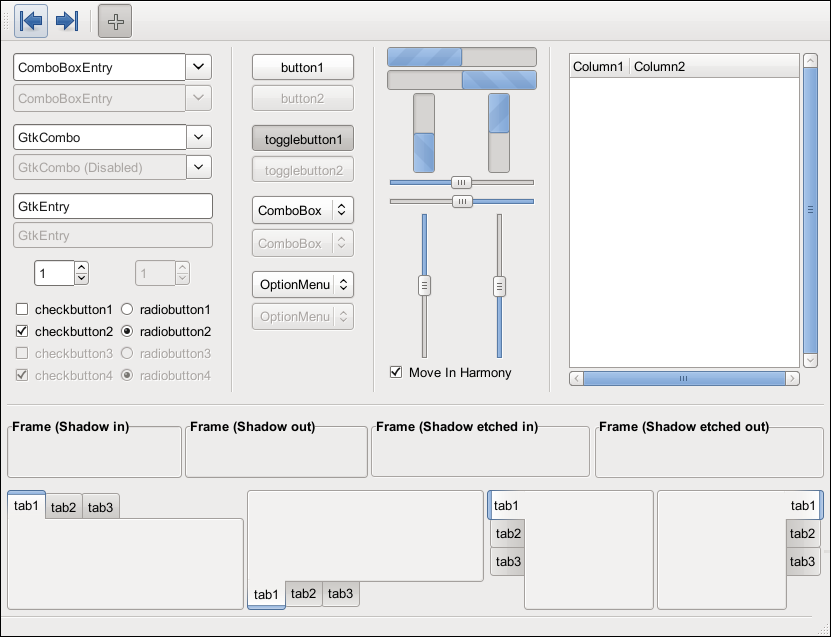
\includegraphics[scale=0.4]{gui1}
\end{figure}

\begin{figure}[h!]
\centering
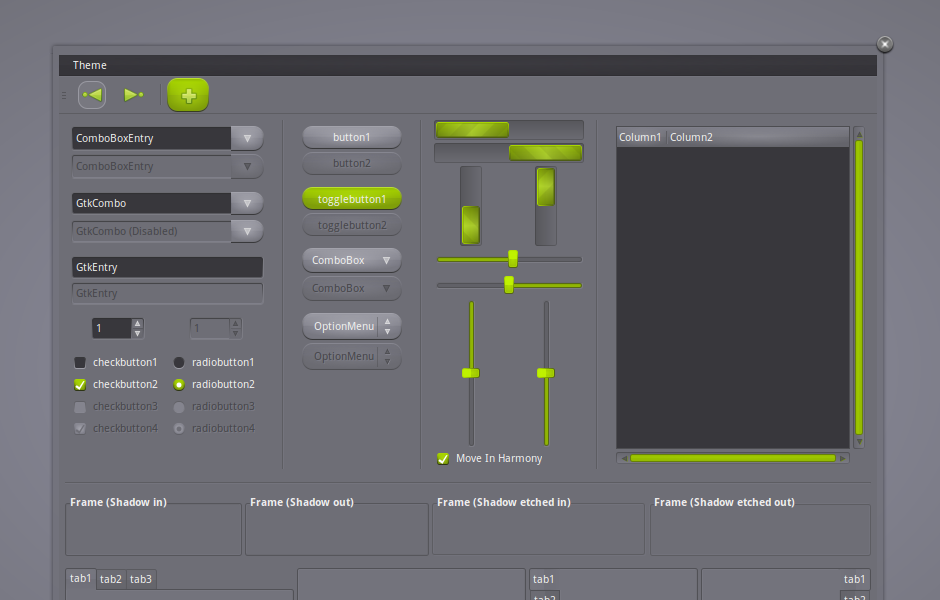
\includegraphics[scale=0.5]{gui2}
\end{figure}

\clearpage

\begin{figure}[h]
\centering
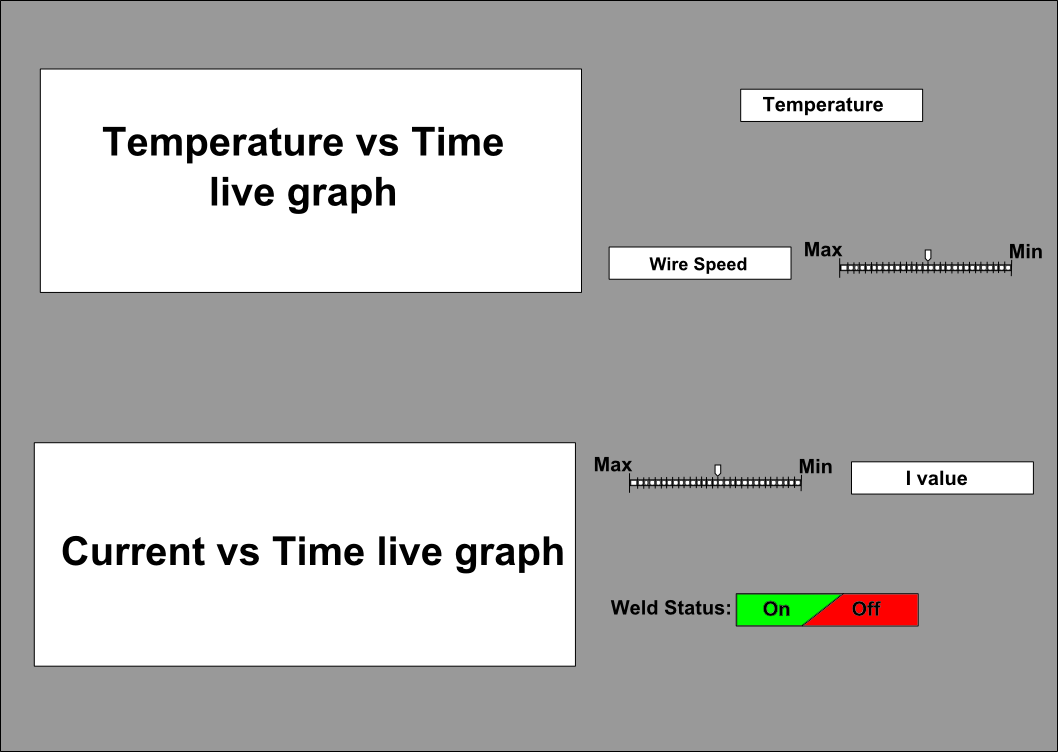
\includegraphics[scale=0.5]{gui}
\caption{Proposed Rough GUI Layout}
\end{figure}

\clearpage

\section{Testing}
\indent Testing was a constant part of this project. Many of the tests were small trouble shooting sessions where we would work on getting a specific piece of hardware or software to work. There were also several tests that were done more methodically, due to their importance of the final outcome. Some of these tests, with their test plans and results, can be seen below.

\subsection{CNC Confirmation Test}

\begin{figure}[h!]
\centering
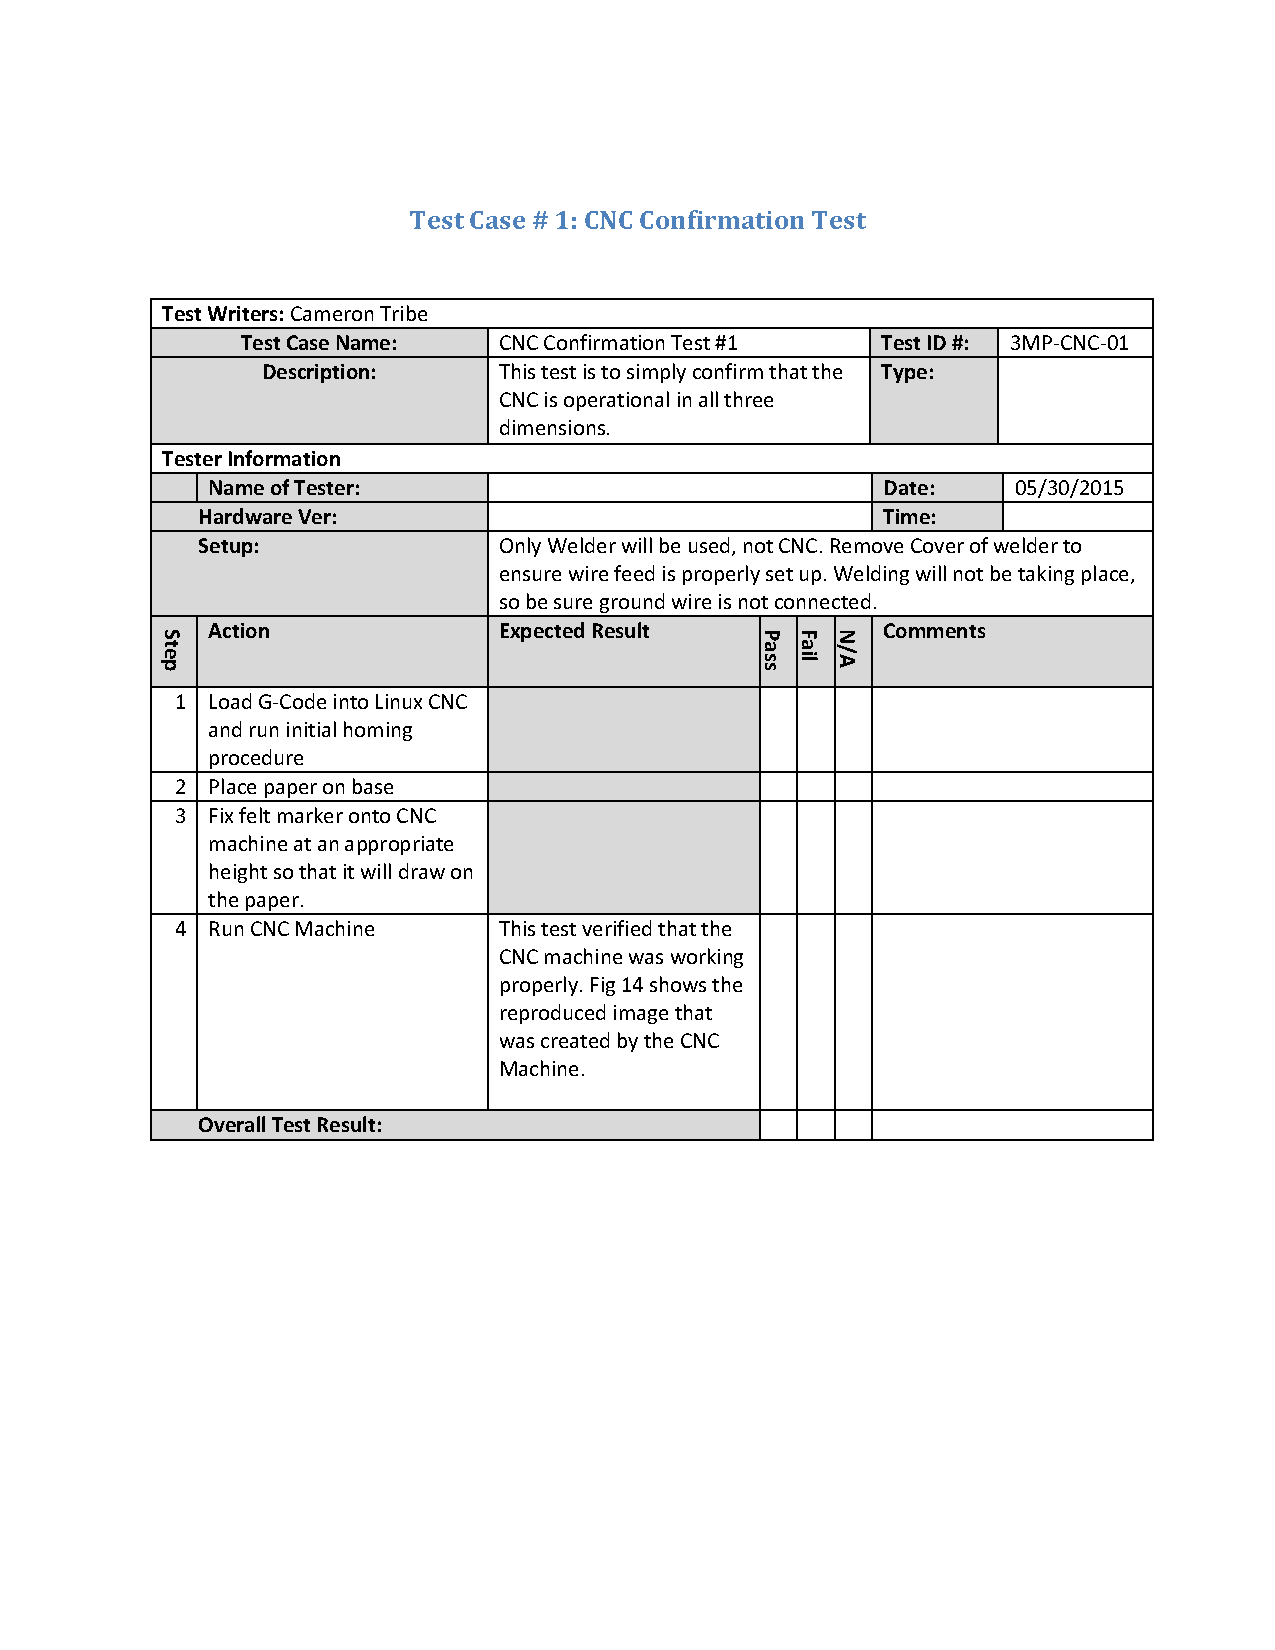
\includegraphics[scale=0.95]{TP1}
\end{figure}

\clearpage

\subsection{Wire Feed Test}

\begin{figure}[h!]
\centering
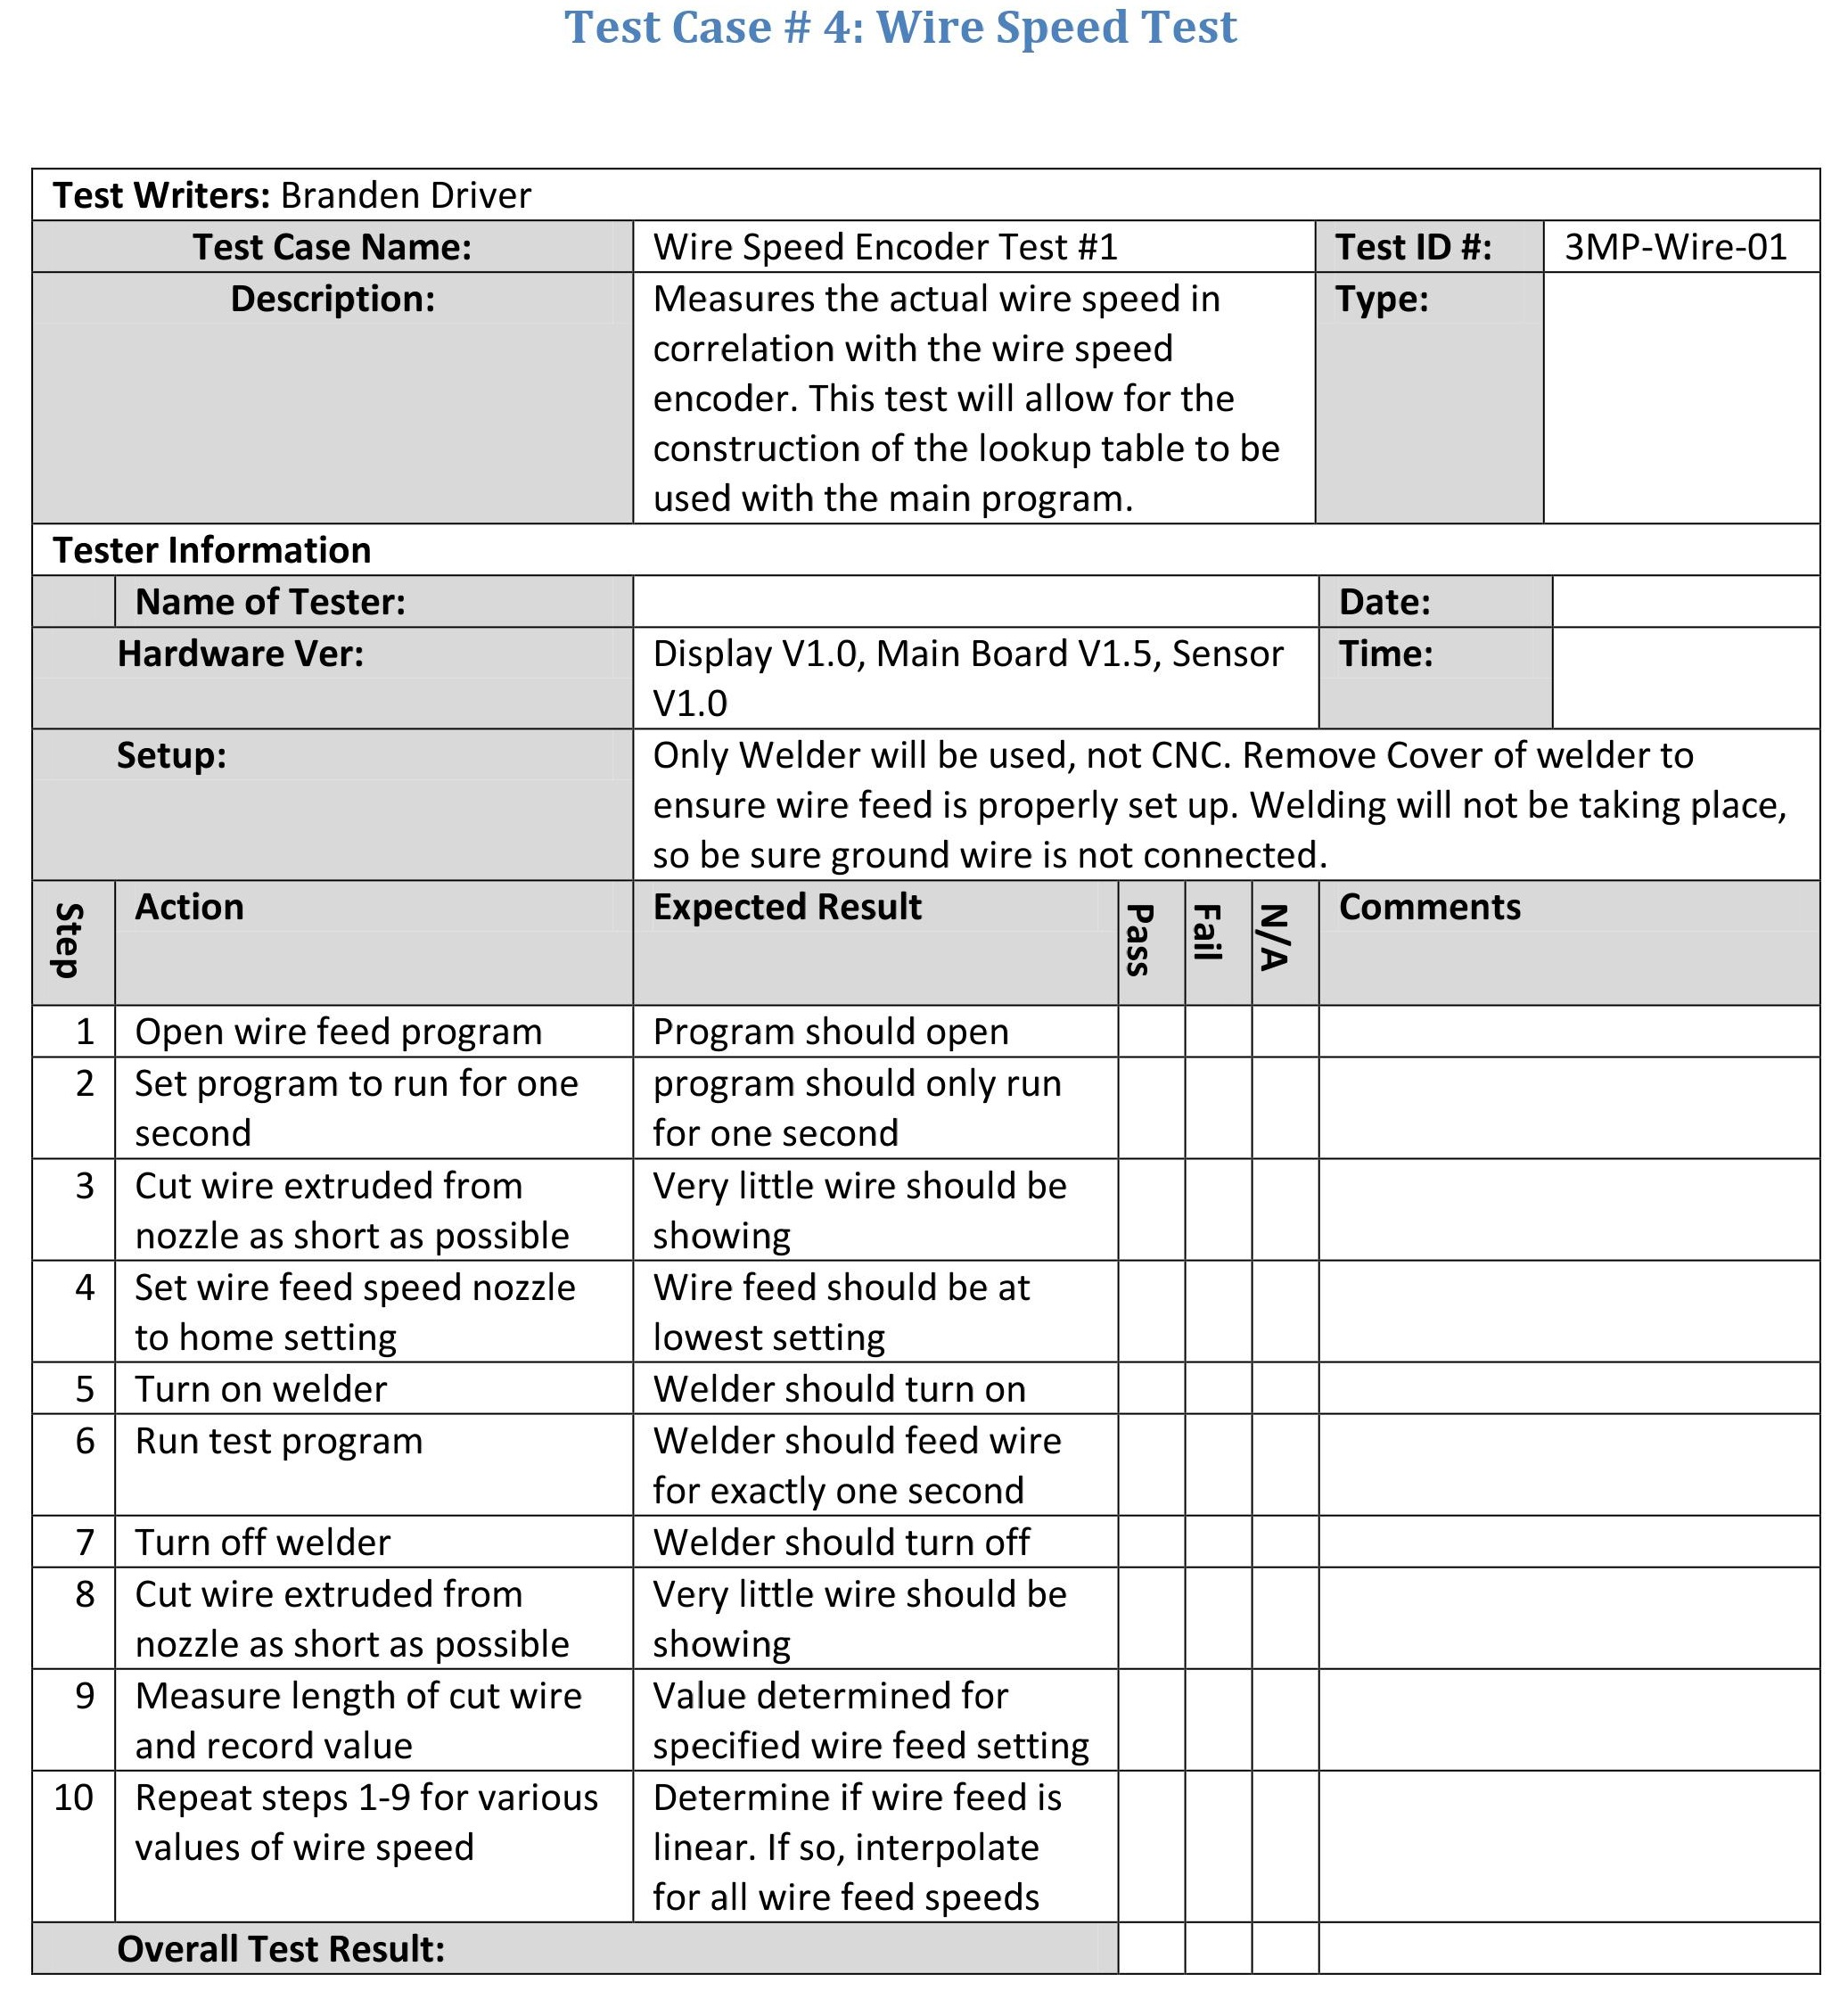
\includegraphics[scale=0.9]{tp-4}
\end{figure}

\clearpage

\begin{center}


\begin{tabular}{ |c|c|c|c|c|c| }


  \hline
  \textbf{Wire Speed (in/s)} & \textbf{Time (sec)} & \textbf{Expected Length (in)} & \textbf{Measured Length (in)} \\ \hline
  0.88 & 3 & 2.64 & 2.56 \\ \hline
  0.90 & 3 & 2.70 & 2.46 \\ \hline
  2.00 & 3 & 6.00 & 6.06 \\ \hline
  3.20 & 3 & 9.60 & 10.10 \\ \hline
  5.50 & 3 & 16.50 & 16.80 \\ \hline
    7.60 & 3 & 22.80 & 23.20 \\ \hline
      9.50 & 3 & 28.50 & 28.06 \\ \hline
      

  
\end{tabular}

\captionof{table}{Linear Velocity Program Test} 



\end{center}


\begin{figure}[!h]
\centering
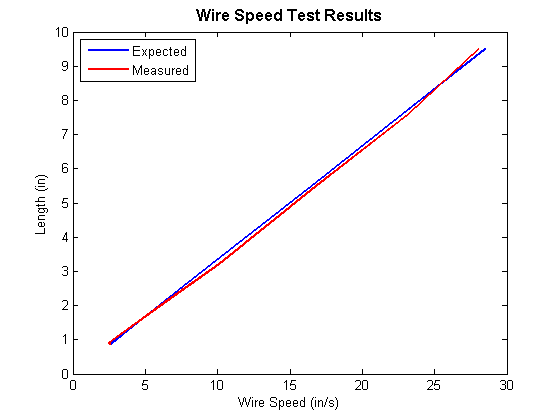
\includegraphics[scale=0.95]{speedplot}
\caption{Wire Speed Test Results}
\end{figure}

\clearpage


\subsection{Weld Quality Test}

\begin{figure}[!h]
\centering
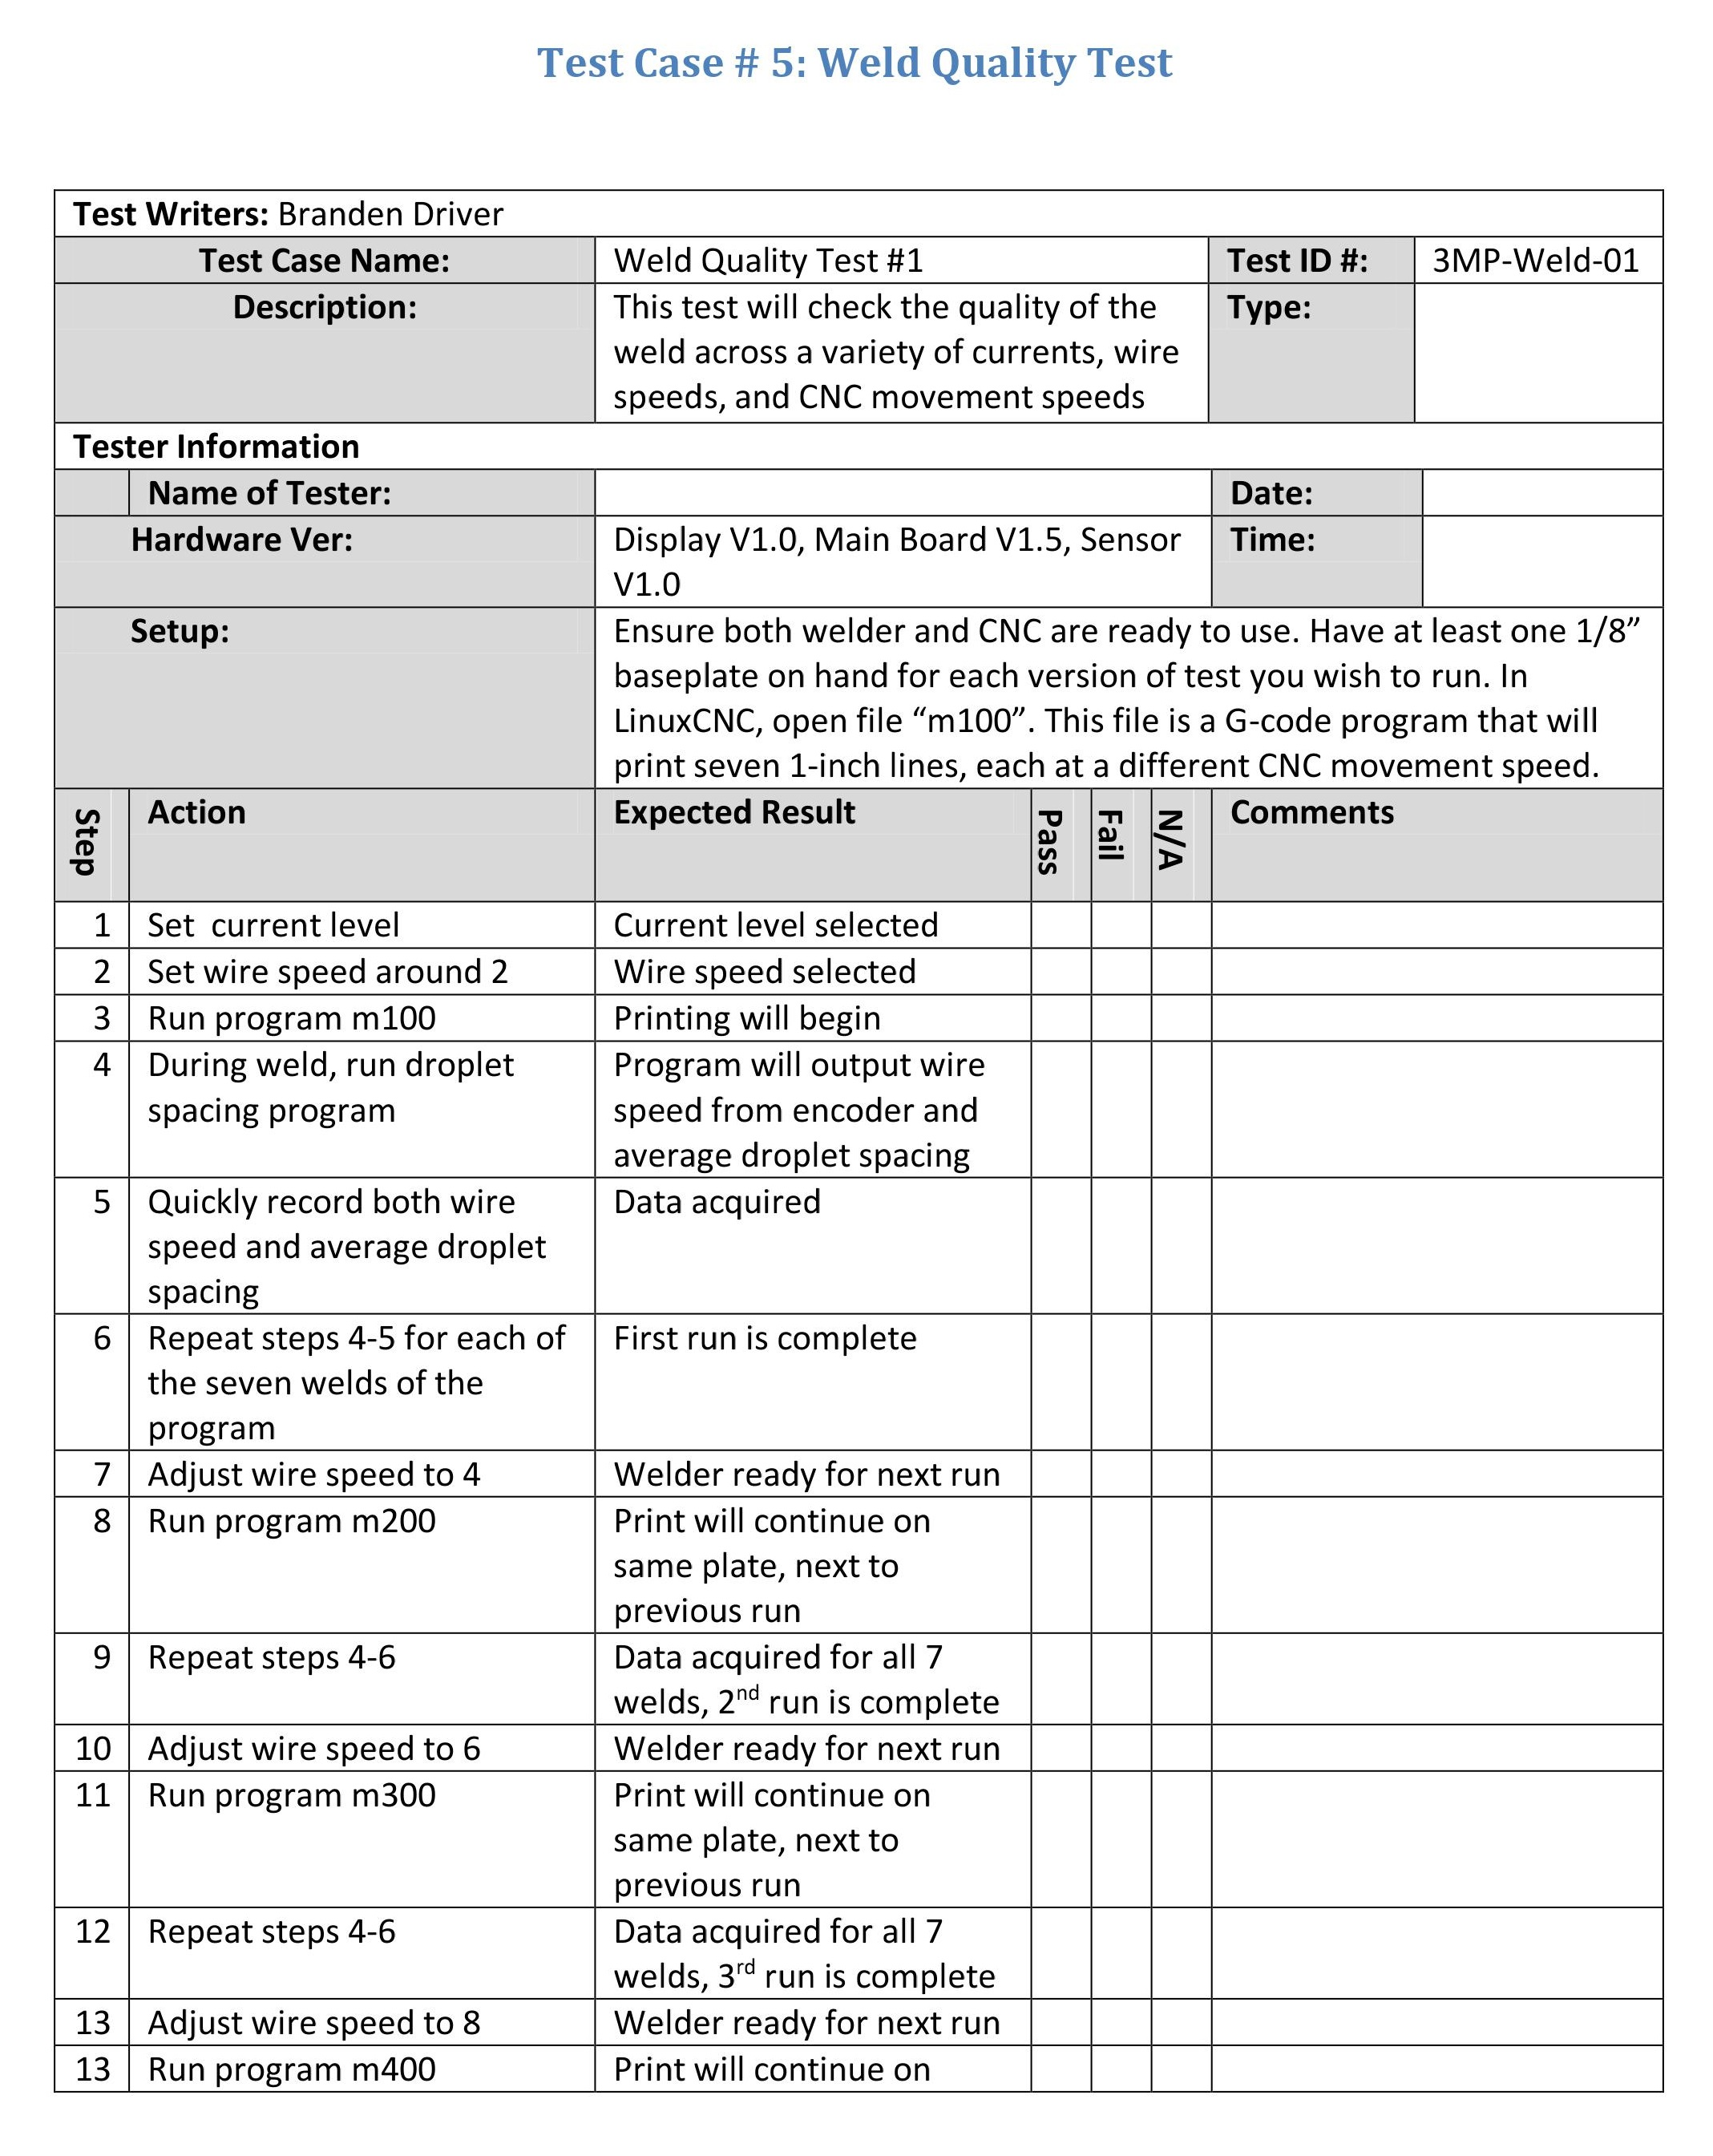
\includegraphics[scale=0.9]{tp-5-1}
\end{figure}


\clearpage

\begin{figure}[!h]
\centering
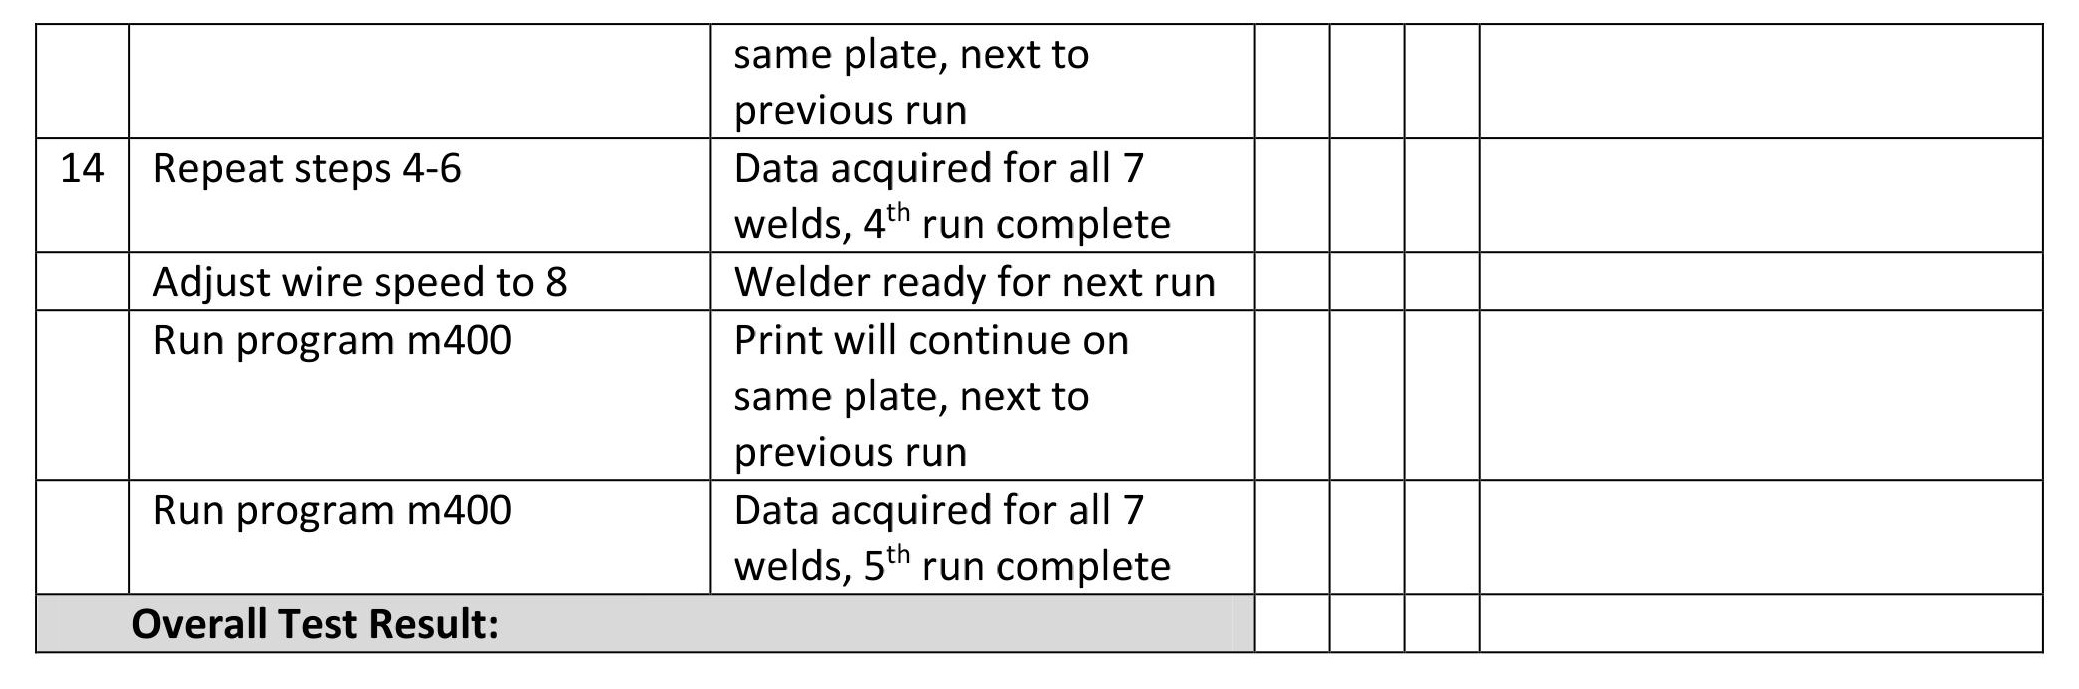
\includegraphics[scale=0.9]{tp-5-2}
\end{figure}


\begin{center}


\begin{tabular}{ |c|c|c|c|c|c| }


  \hline
  \textbf{Wire Speed (in/s)} & \textbf{CNC Speed (in/min)} & \textbf{Avg Droplet Spacing (\textmu s)} \\ \hline
4.21	& 2 &	19047 \\ \hline
4.04 &	3 &	20619 \\ \hline
3.88 &	4 &	22857 \\ \hline
3.98 &	5 &	21978 \\ \hline
4.14 &	6 &	20833 \\ \hline 
3.88 &	7 &	20943 \\ \hline
3.95 &	8 &	18872 \\ \hline \hline
6.02 &	2 &	13119 \\ \hline
5.81 &	3 &	15037 \\ \hline
6.19 &	4 &	14084 \\ \hline
6.06 &	5 &	12539 \\ \hline
5.71 &	6 &	15504 \\ \hline
5.6 &	7 &	10257 \\ \hline
6.54 &	8 &	17621 \\ \hline \hline
7.5	 & 2 &	12820 \\ \hline
7.2 &	3 &	14035 \\ \hline
7.61 &	4 &	14760 \\ \hline
7.67 &	5 &	15267 \\ \hline
7.61 &	6 &	17167 \\ \hline
7.45 &	7 &	11594 \\ \hline
6.95 &	8 &	10790 \\ \hline \hline
8.99 &	2 &	11364 \\ \hline 
8.82 &	3 &	13114 \\ \hline
9.58 &	4 &	11940 \\ \hline
10 &	5 &	11765 \\ \hline
8.5 &	6 &	10106 \\ \hline
9.47 &	7 &	12751 \\ \hline
9.84 &	8 &	n/a \\ \hline


  
\end{tabular}

%\captionof{table}{Plate 1} 


\end{center}


\clearpage

\begin{center}


\begin{tabular}{ |c|c|c|c|c|c| }


  \hline
  \textbf{Wire Speed (in/s)} & \textbf{CNC Speed (in/min)} & \textbf{Avg Droplet Spacing (\textmu s)} \\ \hline

11 &	2 &	10582 \\ \hline
10.86 &	3 &	9557 \\ \hline
10.65 &	4 &	10811 \\ \hline
10.03 &	5 &	12270 \\ \hline
11.05 &	6 &	11007 \\ \hline
11.49 &	7 &	12012 \\ \hline
11.85 &	8 &	11695 \\ \hline



  
\end{tabular}

\captionof{table}{Plate 1} 


\end{center}



\begin{center}

\begin{tabular}{ |c|c|c|c|c|c| }


  \hline
  \textbf{Wire Speed (in/s)} & \textbf{CNC Speed (in/min)} & \textbf{Avg Droplet Spacing (\textmu s)} \\ \hline
3.48 &	2 &	20014 \\ \hline
3.47 &	3 &	23121 \\ \hline
3.3 &	4 &	23530 \\ \hline
3.3 &	5 &	27398 \\ \hline
2.96 &	6 &	26845 \\ \hline
3.39 &	7 &	29646 \\ \hline
3.42 &	8 &	30534 \\ \hline \hline
4.07 &	2 &	24342 \\ \hline
4.19 &	3 &	19802 \\ \hline
3.95 &	4 &	17467 \\ \hline
3.86 &	5 &	18868 \\ \hline
4.14 &	6 &	14545 \\ \hline
4.09 &	7 &	13333 \\ \hline
3.99 &	8 &	19900 \\ \hline \hline
6.55 &	2 &	11267 \\ \hline
6.8 &	3 &	11173 \\ \hline
7.23 &	4 &	12012 \\ \hline
6.49 &	5 &	9788 \\ \hline
6.38 &	6 &	9389 \\ \hline
6.3 &	7 &	9216 \\ \hline
6.68 &	8 &	9009 \\ \hline \hline
9.8 &	2 &	9442 \\ \hline
9.57 &	3 &	8928 \\ \hline
10.28 &	4 &	9456\\ \hline
10.89 &	5 &	9280 \\ \hline
9.89 &	6 &	9204 \\ \hline
9.83 &	7 &	8050 \\ \hline
10.01 &	8 &	9456 \\ \hline





  
\end{tabular}

%\captionof{table}{Plate 2} 

\end{center}

\clearpage

\begin{center}

\begin{tabular}{ |c|c|c|c|c|c| }


  \hline
  \textbf{Wire Speed (in/s)} & \textbf{CNC Speed (in/min)} & \textbf{Avg Droplet Spacing (us)} \\ \hline

11.49 &	2 &	8677 \\ \hline
11.46 &	3 &	8340 \\ \hline
11.43 &	4 &	8752 \\ \hline
11.75 &	5 &	8798 \\ \hline
11.6 &	6 &	9302 \\ \hline
11.53 &	7 &	9029 \\ \hline
11.69 &	8 &	9132 \\ \hline 




  
\end{tabular}

\captionof{table}{Plate 2} 

\end{center}

\clearpage

\begin{center}

\begin{tabular}{ |c|c|c|c|c|c| }


  \hline
  \textbf{Wire Speed (in/s)} & \textbf{CNC Speed (in/min)} & \textbf{Avg Droplet Spacing (us)} \\ \hline
5.34 &	2 &	12658 \\ \hline
4.9	& 3 &	14053 \\ \hline
4.97 &	4 &	12317 \\ \hline
5.18 &	5 &	16461 \\ \hline
4.53 &	6 &	11019 \\ \hline
4.83 &	7 &	79756 \\ \hline
n/a &	8 &	n/a \\ \hline \hline
7.12 &	2 &	9876 \\ \hline
6.93 &	3 &	9959 \\ \hline
7.22 &	4 &	10315 \\ \hline
6.82 &	5 &	9527 \\ \hline
6.74 &	6 &	9195 \\ \hline
6.8 &	7 &	9227 \\ \hline
6.87 &	8 &	9852 \\ \hline \hline
9.3 &	2 &	8948 \\ \hline
9.19 &	3 &	9091 \\ \hline
9.42 &	4 &	9599 \\ \hline
9.26 &	5 &	9466 \\ \hline
9.31 &	6 &	9204 \\ \hline
n/a &	7 &	n/a \\ \hline
9.16 &	8 &	8180 \\ \hline \hline
12.58 &	2 &	8421 \\ \hline
12.41 &	3 &	8445 \\ \hline
12.77 &	4 &	8465 \\ \hline
12.74 &	5 &	8792 \\ \hline
12.56 &	6 &	8620 \\ \hline
12.66 &	7 &	8602 \\ \hline
12.82 &	8 &	8714 \\ \hline \hline
14.67 &	2 &	8477 \\ \hline
15.19 &	3 &	8585 \\ \hline
14.87 &	4 &	8756 \\ \hline
14.69 &	5 &	8547 \\ \hline
14.89 &	6 &	8677 \\ \hline
14.32 &	7 &	8639 \\ \hline
14.65 &	8 &	8403 \\ \hline


 
\end{tabular}

\captionof{table}{Plate 3} 

\end{center}

\clearpage


\begin{center}

\begin{tabular}{ |c|c|c|c|c|c| }


  \hline
  \textbf{Wire Speed (in/s)} & \textbf{CNC Speed (in/min)} & \textbf{Avg Droplet Spacing (us)} \\ \hline
3.83 &	4 &	9013 \\ \hline
3.85 &	4.5 &	9828 \\ \hline
3.89 &	5 &	9780 \\ \hline
4 &	5.5 &	11662 \\ \hline
3.96 &	6 &	9552 \\ \hline
3.97 &	6.5 &	10447 \\ \hline
3.8 &	7 &	10371 \\ \hline \hline
4.66 &	4 &	9860 \\ \hline
5.07 &	4.5 &	9780 \\ \hline
4.61 &	5 &	9569 \\ \hline
4.64 &	5.5 &	9238 \\ \hline
4.55 &	6 &	9501 \\ \hline
4.59 &	6.5 &	9099 \\ \hline
4.75 &	7 &	9287 \\ \hline \hline
4.77 &	4 &	9909 \\ \hline
4.63 &	4.5 &	10032 \\ \hline
4.6 &	5 &	9029 \\ \hline
5.19 &	5.5 &	9784 \\ \hline
4.56 &	6 &	n/a \\ \hline
4.67 &	6.5 &	9756 \\ \hline
4.65 &	7 &	9434 \\ \hline \hline
5.35 &	4 &	9645 \\ \hline
5.37 &	4.5 &	10025 \\ \hline
5.34 &	5 &	9758 \\ \hline
5.35 &	5.5 &	10554 \\ \hline
5.61 &	6 &	9546 \\ \hline
5.17 &	6.5 &	9961 \\ \hline
5.36 &	7 &	9307 \\ \hline \hline
6.1 &	4 &	8877 \\ \hline
5.98 &	4.5 &	9412 \\ \hline
6.09 &	5 &	9615 \\ \hline
6.03 &	5.5 &	9350 \\ \hline
6.76 &	6 &	9863 \\ \hline
6.35 &	6.5 &	10474 \\ \hline
6.15 &	7 &	9198 \\ \hline



 
\end{tabular}

\captionof{table}{Plate 4} 

\end{center}

\clearpage


\begin{center}

\begin{tabular}{ |c|c|c|c|c|c| }


  \hline
  \textbf{Wire Speed (in/s)} & \textbf{CNC Speed (in/min)} & \textbf{Avg Droplet Spacing (us)} \\ \hline
  
4.09 &	4.8 &	9195 \\ \hline
4.47 &	5 &	9737 \\ \hline
4.28 &	5.2 &	10126 \\ \hline
3.39 &	5.4 &	9623 \\ \hline
4.25 &	5.6 &	9740 \\ \hline
4.09 &	5.8 &	9876 \\ \hline
3.98 &	6 &	9262 \\ \hline \hline
4.61 &	4.8 &	9953 \\ \hline
4.38 &	5 &	9761 \\ \hline
4.56 &	5.2 &	9389 \\ \hline
4.77 &	5.4 &	10582 \\ \hline
4.56 &	5.6 &	9661 \\ \hline
4.53 &	5.8 &	9625 \\ \hline
4.2 &	6 &	9183 \\ \hline \hline
4.71 &	4.8 &	9266 \\ \hline
4.61 &	5 &	9569 \\ \hline
4.94 &	5.2 &	9479 \\ \hline
4.62 &	5.4 &	9376 \\ \hline
4.92 &	5.6 &	9184 \\ \hline
4.89 &	5.8 &	9324 \\ \hline
4.86 &	6 &	9546 \\ \hline \hline
5.21 &	4.8 &	8994 \\ \hline
4.97 &	5 &	9111 \\ \hline
5.31 &	5.2 &	9595 \\ \hline
5.21 &	5.4 &	9324 \\ \hline
5.02 &	5.6 &	9117 \\ \hline
5.1 &	5.8 &	9153 \\ \hline
5.26 &	6 &	9456 \\ \hline \hline
5.37 &	4.8 &	9111 \\ \hline
5.56 &	5 &	9376 \\ \hline
5.51 &	5.2 &	9456 \\ \hline
	& 5.4	 & \\ \hline
	& 5.6 & \\ \hline	
	& 5.8 & \\ \hline	
	& 6 & \\ \hline	




 
\end{tabular}

\captionof{table}{Plate 5} 

\end{center}

\clearpage

\begin{center}

\begin{tabular}{ |c|c|c|c|c|c| }


  \hline
  \textbf{Wire Speed (in/s)} & \textbf{CNC Speed (in/min)} & \textbf{Avg Droplet Spacing (us)} \\ \hline
  
2.57 &	2 &	12903 \\ \hline
2.55 &	3 &	12195 \\ \hline
2.59 &	4 &	13559 \\ \hline
2.48 &	5 &	15873 \\ \hline
2.79 &	6 &	15269 \\ \hline
2.62 &	7 &	16953 \\ \hline
2.63 &	8 &	14760 \\ \hline \hline
3.38 &	2 &	10392 \\ \hline
3.27 &	3 &	10309 \\ \hline
3.72 &	4 &	11396 \\ \hline
3.7 &	5 &	12232 \\ \hline
3.39 &	6 &	11950 \\ \hline
3.45 &	7 &	11954 \\ \hline
3.52 &	8 &	14100 \\ \hline \hline
4.12 &	2 &	9464 \\ \hline
4 &	3 &	9662 \\ \hline
3.98 &	4 &	10000 \\ \hline
4.26 &	5 &	10256 \\ \hline
4.54 &	6 &	10816 \\ \hline
4.41 &	7 &	10816 \\ \hline
3.91 &	8 &	11665 \\ \hline \hline
4.47 &	2 &	9117 \\ \hline
4.48 &	3 &	8960 \\ \hline
4.47 &	4 &	9284 \\ \hline
4.84 &	5 &	9756 \\ \hline
4.39 &	6 &	9112 \\ \hline
4.98 &	7 &	11628 \\ \hline
4.37 &	8 &	11338 \\ \hline \hline
n/a &	2 &	n/a \\ \hline
4.64 &	3 &	8658 \\ \hline
4.67 &	4 &	8928 \\ \hline
4.71 &	5 &	8565 \\ \hline
5.07 &	6 &	11111 \\ \hline
4.99 &	7 &	10638 \\ \hline
5 &	8 &	10340 \\ \hline	




 
\end{tabular}

\captionof{table}{Plate 6} 

\end{center}

\clearpage

\subsection{Degrees to Wire Speed Test}
Determining the amount to turn the wire speed knob to increase the overall wire speed by exactly one inch was another test that was completed. This was done by figuring out the amount of time to leave the motor on to turn it 30$^\circ$ and measuring the difference in wire speeds. Multiple iterations of this test gave us a good average value, which came out to be about 40$^\circ$ per inch per second. This value was then used to determine how long to turn the stepper motor on, so as to reach a final desired wire speed setting.

\begin{center}
	\begin{tabu}{ |c|c|c|c|c|c|c| }
			  \hline
			  \thead{Run \#} & \thead{Initial \\ Wire \\ Speed \\ (in/s)} & \thead{Final \\ Wire \\ Speed \\ (in/s)} & \thead{Turn Amount \\ (deg)} &	\thead{Ratio \\ (deg/(in/s))}	 & \thead{Time/deg \\ (us)} &	\thead{Pulse \\ On Time \\ (us)} \\ \hline
			  
			Run 1	& 0.3 &	1.1 &	30 &	37.5 &	22222 &	666660 \\ \hline
			Run 2	& 1.1 &	1.8 &	30 &	42.85714286 &	22222 &	666660 \\ \hline
			Run 3 &	1.8 &	2.5 &	30 &	42.85714286 &	22222 &	666660  \\ \hline
			Run 4 &	2.5 &	3.3 &	30 &	37.5 &	22222 &	666660 \\ \tabucline[2pt]{-}
			Run 5 &	1.9 &	3 &	45 &	40.90909091 &	22222 &	999990 \\ \hline
			Run 6 &	3 &	4.2 &	45 &	37.5 &	22222 &	999990 \\ \hline
			Run 7 &	1.2 &	2.3 &	45 &	40.90909091 &	22222 &	999990 \\ \hline
			Run 8 &	2.3 &	3.4 &	45 &	40.90909091 &	22222 &	999990 \\ \tabucline[2pt]{-}
			Run 9 &	0.9 &	2.4 &	60 &	40 &	22222 &	1333320 \\ \hline
			Run 10 &	2.4 &	3.9 &	60 &	40 &	22222 &	1333320 \\ \hline
			Run 11 &	3.9 &	5.5 &	60 &	37.5 &	22222 &	1333320 \\ \hline
			Run 12 &	3.4 &	5 &	60 &	37.5 &	22222 &	1333320 \\ \tabucline[2pt]{-}
			Run 13 &	1 &	7 &	235 &	39.16666667 &	22222 &	5222170 \\ \tabucline[2pt]{-}
			       &	  &   & \thead{Average} & \thead{39.66179654} & & \\ \hline
	\end{tabu}
	\captionof{table}{Test Results to Detemine Degrees to Turn for 1-inch Increase in Wire Speed}
\end{center}
\clearpage


\section{Photos and Videos of Progress}

Demo of the Printer

\href{https://www.youtube.com/watch?v=Ypetogtn1Iw}{https://www.youtube.com/watch?v=Ypetogtn1Iw}\\

One of the fist things done in this project was to confirm the operation of the CNC machine. To do this, G-Code of a 2D image was uploaded to the machine. A felt marker was used to draw the image below. \\

\begin{figure}[!ht]
\centering
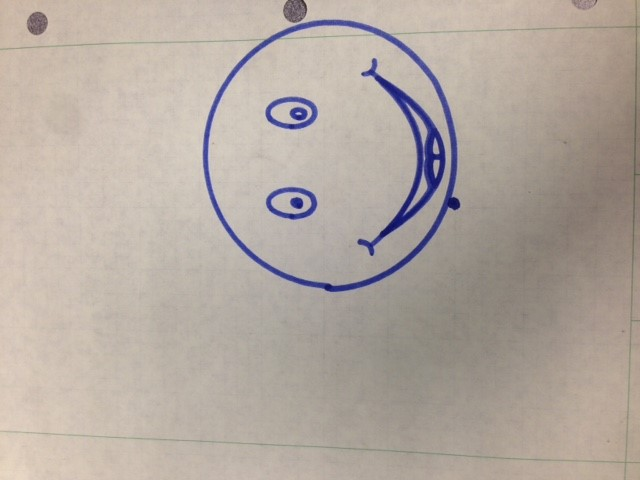
\includegraphics[scale=0.6]{pic1}
\caption{CNC Test Results}
\end{figure}

Next, we fitted the welder to the machine, and placed a metal base plate to weld on. To control the welder we just used our hand to active the weld while the machine was moving.

\clearpage


\begin{figure}[!ht]
\centering
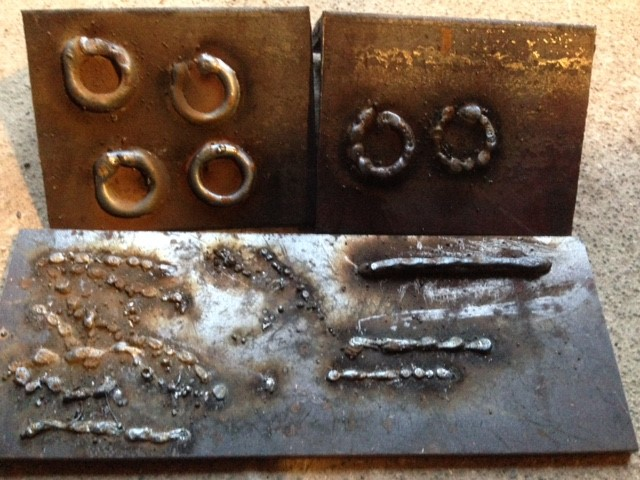
\includegraphics[width=0.63\textwidth]{pic2}
\caption{Initial Test Results - No Control}
\end{figure}

After this, we connected the relay switch circuit in parallel with the manual welder switch, using G-Code to activate the switch. Shown Below is the result of letting the CNC Machine control the weld.

\begin{figure}[!htp]
\centering
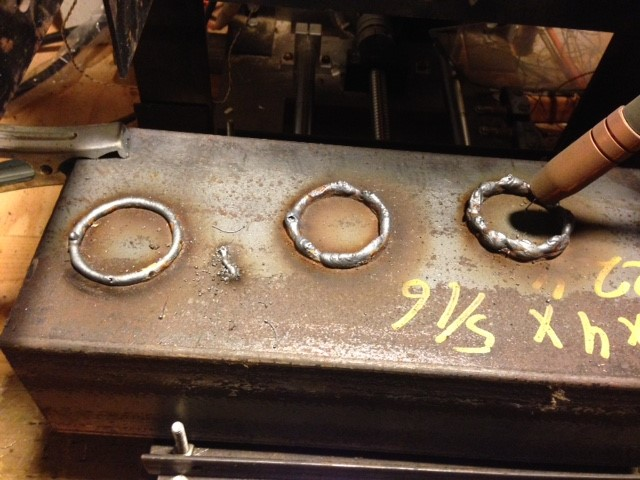
\includegraphics[width=0.63\textwidth]{pic3}
\caption{Initial Test Results - No Control}
\end{figure}



\bigskip
\begin{figure}[!ht]
\centering
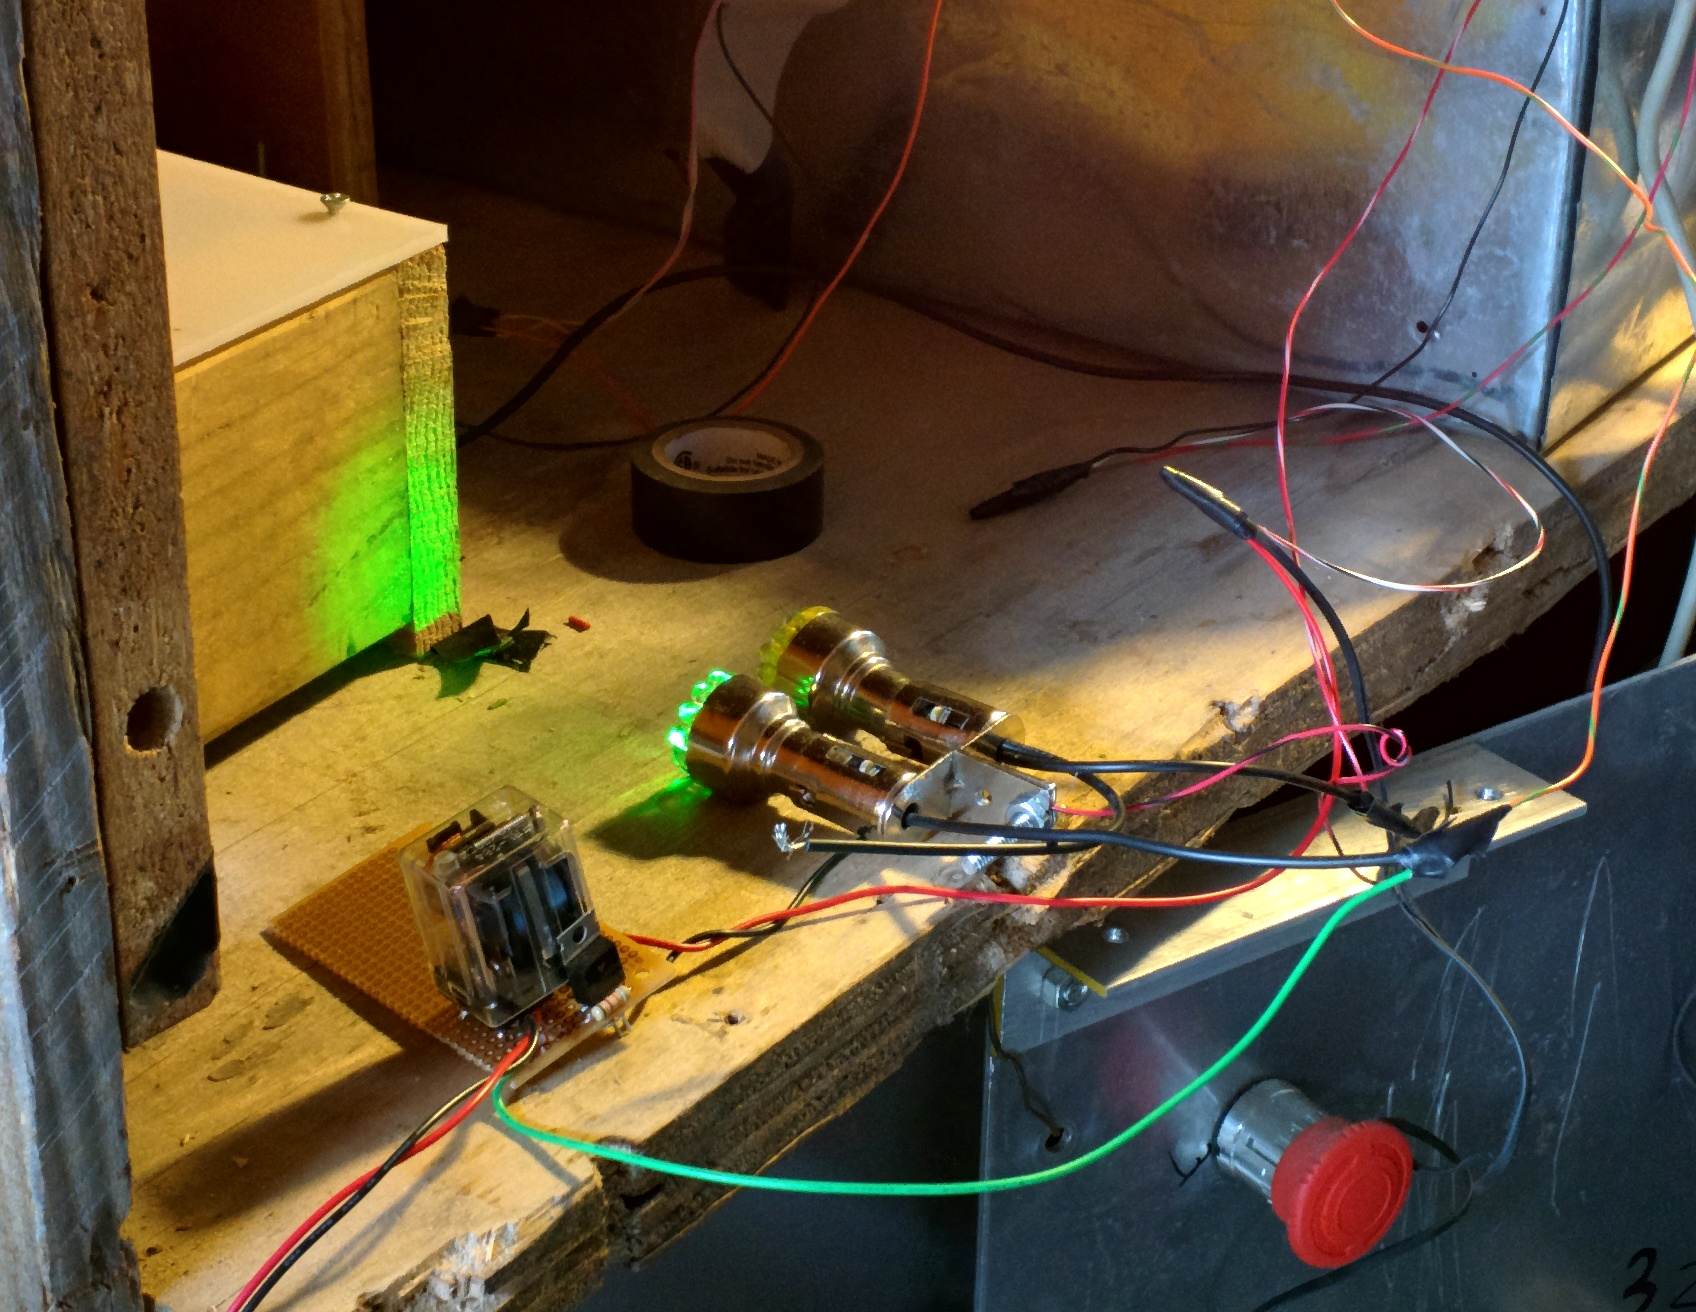
\includegraphics[width=.75\textwidth]{IMG_20150410_163658}
\caption{Prototype Relay and Indication Module}
\end{figure}




\begin{figure}[!ht]
\centering
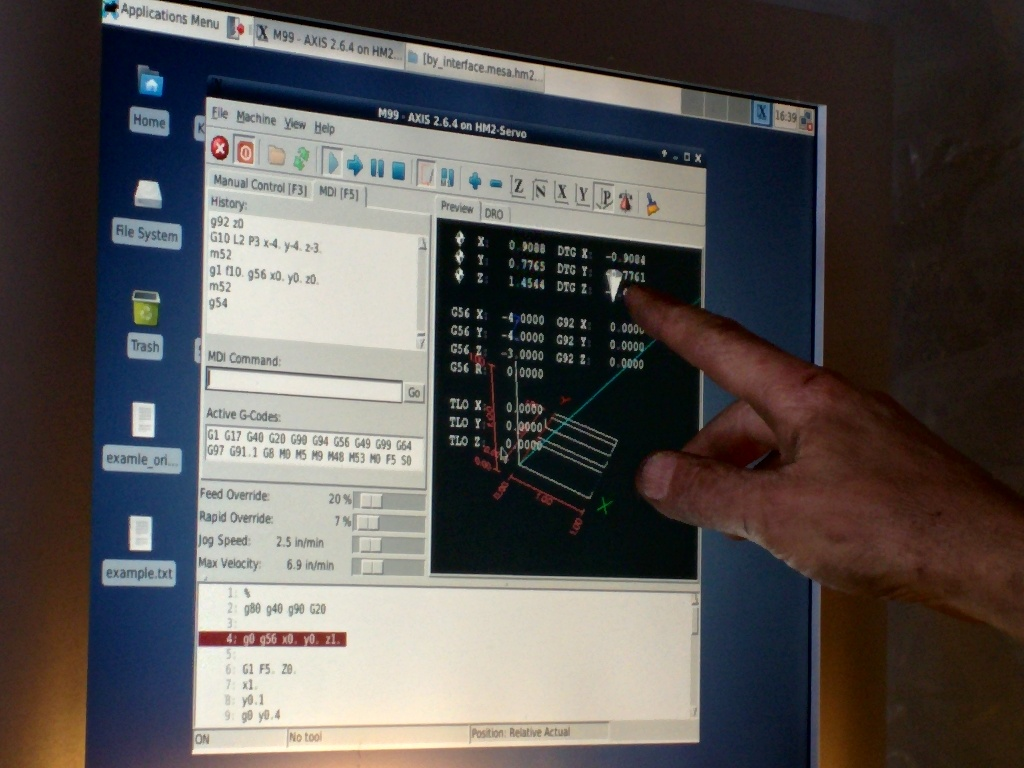
\includegraphics[width=.75\textwidth]{IMG_20150410_163626}
\caption{Linux CNC Interface}
\end{figure}



\begin{figure}[!ht]
\centering
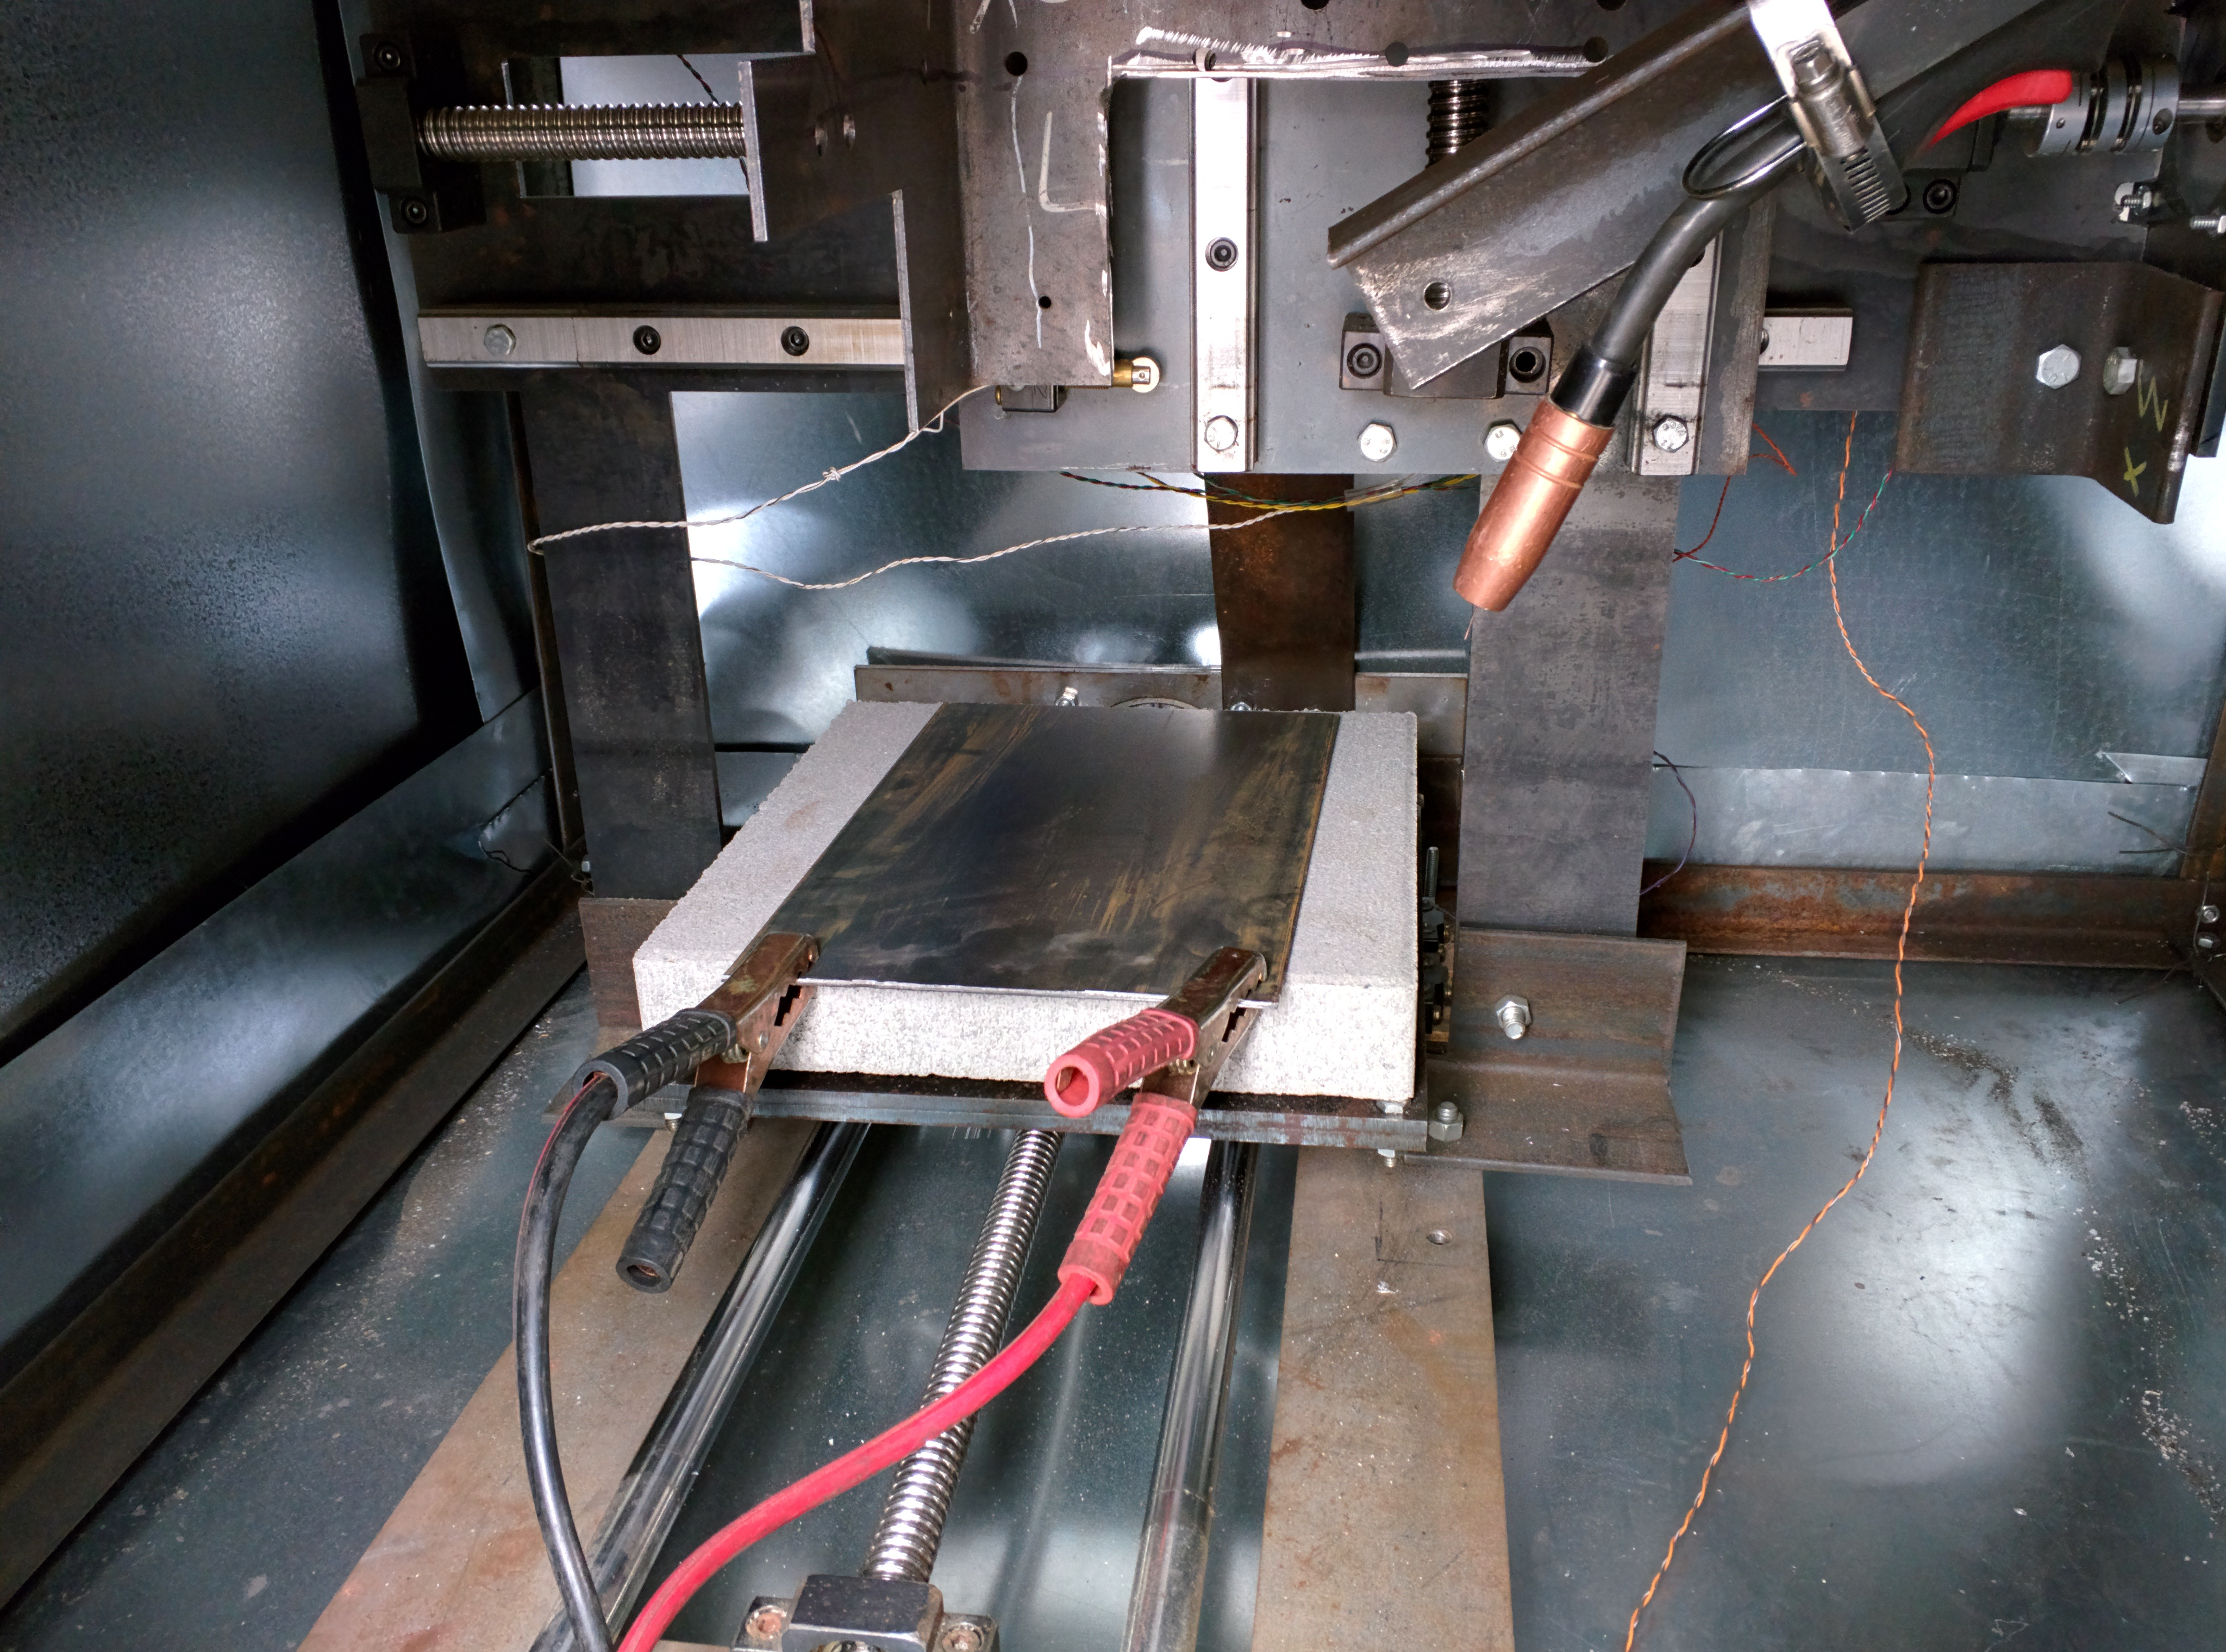
\includegraphics[width=.75\textwidth]{IMG_20150410_163441}
\caption{Baseplate Weld Setup}
\end{figure}




\begin{figure}[!ht]
\centering
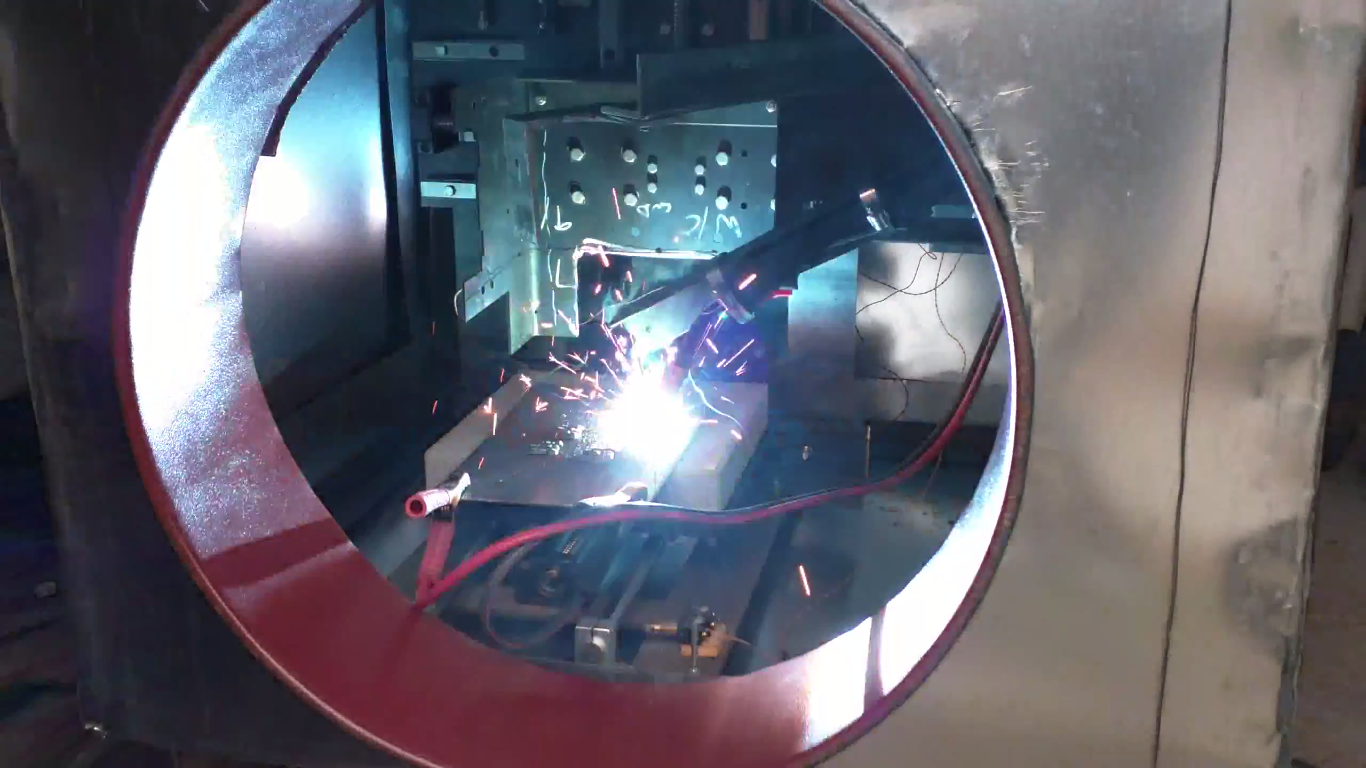
\includegraphics[width=.75\textwidth]{23}
\caption{Printer in Deposition Mode}
\end{figure}




\clearpage

\section{Bill of Materials (BOM)}

\begin{adjustwidth}{-2cm}{-2cm}

\begin{center}


\begin{tabular}{ |c|c|c|c|c|c| }


  \hline
  \textbf{Item} & \textbf{Quantity} & \thead{Part \\ Number} & \textbf{Mfg} & \textbf{Price} & \textbf{Description} \\  \hline
  \multicolumn{1}{|l|}{CNC Machine} & 1 & NPN & \makecell{Aram \\ Kasparov} & $\sim$\$500 &  \\ \hline 
  - X-Stepper Motor & 1 & \makecell{IG34CK-32-\\IE8192-SB213} & \makecell{Servo \\ Dynamics} & \$400 & \makecell{Stepper Motor \\ for the X axis}  \\ \hline
  - Y-Stepper Motor & 1 & HJ130E8-1308 & \makecell{Servo \\ Dynamics} & \$800 & \makecell{Stepper Motor \\ for the Y axis}  \\ \hline
  - Z-Stepper Motor & 1 & \makecell{IG34CK-32-\\IE8192-SB213} & \makecell{Servo \\ Dynamics} & \$450 & \makecell{Stepper Motor \\ for the Z axis} \\ \hline
  - Motor Driver & 3 & SD94 & \makecell{Servo \\ Dynamics} & \$550 & \makecell{Motor driver for \\ XYZ axis motors.} \\ \hline \hline
  
  
  \multicolumn{1}{|l|}{Limit and Home Switches} & 11 & Z15G1308 & HIGHLY & \$10 & \makecell{Any limit and \\ home switch used \\ on the machine}  \\ \hline
 
  \multicolumn{1}{|l|}{PCI I/O Card} & 1 & 5I20 & \makecell{Mesa \\ Electronics} & \$250 & \makecell{Part of the \\ CNC system}   \\ \hline
  \multicolumn{1}{|l|}{Servo Interface Card} & 1 & 7i33 & \makecell{Mesa \\ Electronics} & \$100 & \makecell{Interface Card for \\ communicating with \\ servo motors}
   \\ \hline
  \multicolumn{1}{|l|}{Isolated I/O Card} & 2 & 7i37 & \makecell{Mesa \\ Electronics} & \$100 & \makecell{I/O card used \\ for limit and \\ home switches}
  \\ \hline \hline
  
  \multicolumn{1}{|l|}{\textbf{50 Pin Breakout Board}} & 3 & NPN & & $\sim$\$10 & \makecell{To connect to analog \\ \& digital channels of \\ the Sensoray} \\ \hline  
  \multicolumn{1}{|c|}{Screw Terminals} & & NPN & \makecell{Capstone 2015 \\ Team} & & \\ \hline  
  \multicolumn{1}{|c|}{50 Pin Connector} & & NPN & \makecell{Capstone 2015 \\ Team} & & \\ \hline  
  
  
  
  
  
  
  
\end{tabular}

\end{center}




\clearpage

\end{adjustwidth}


\begin{adjustwidth}{-2cm}{-2cm}

\begin{center}


\begin{tabular}{ |c|c|c|c|c|c|c| }


  \hline
  
  \textbf{Item} & \textbf{Quantity} & \thead{Part \\ Number} & \textbf{Mfg} & \textbf{Price} & \textbf{Description} \\  \hline
  
 
\multicolumn{1}{|l|}{\textbf{26 Pin Breakout Board}} & 2 & NPN & & $\sim$\$10 & \makecell{To connect to the \\ counter channels \\ of the Sensoray} \\ \hline  
  \multicolumn{1}{|c|}{Screw Terminals} & & NPN & \makecell{Capstone 2015 \\ Team} & & \\ \hline  
  \multicolumn{1}{|c|}{26 Pin Connector} & & NPN & \makecell{Capstone 2015 \\ Team} & & \\ \hline  \hline
  	  
  	  
 \multicolumn{1}{|l|}{Incremental Encoder} & 1 & \makecell{S5-5000-250-\\IE-D-B} & \makecell{US \\ Digital} & \$140 & \makecell{Used for measuring \\ the wire speed \\ of the welder}   \\ \hline  

  
  \multicolumn{1}{|l|}{PCIe DAQ} & 1 & 826 & Sensoray & \$677 & \makecell{PCI I/O Card with \\ Digital and Analog I/O}   \\ \hline  
  
  \multicolumn{1}{|l|}{Temperature Sensor} & 1 & 1MH1-CF4 & \makecell{Micro-\\Epsilon} & \$1400 & Temp range x-x    \\ \hline  
  
  \multicolumn{1}{|l|}{Current Sensor} & 1 & c20058 & Honeywell & \$30 &  Outputs a single Voltage  \\ \hline
  
  
   
 
 
 
  \multicolumn{1}{|l|}{MIG Welder} & \multicolumn{1}{c|}{1} & \multicolumn{1}{c|}{MIG 180} & \makecell{Chicago \\ Electric} & \$270 & \makecell{Wire Feed Welder \\ that uses \\ inert shielding gas}   \\ \hline
  \multicolumn{1}{|l|}{Motor Controller} & \multicolumn{1}{c|}{2} & \multicolumn{1}{c|}{KL-5056D} & \makecell{Keling \\ Technology \\ Inc} & \$80 & \makecell{To control the \\ motors on the \\ welder control knobs}
   \\ \hline
  
  \multicolumn{1}{|l|}{Stepper Motors} & 1 & \makecell{KL23H2100-\\35-4B} & \makecell{Keling \\ Technology \\ Inc} & \$50 & \makecell{To control the knobs \\ on the welder}   \\ \hline
  
  \multicolumn{1}{|l|}{PWM Module} & 1 & THC-AD  & \makecell{Mesa \\ Electronics} & \$80 & \makecell{To externally set \\ CNC speed}   \\ \hline
  
  \multicolumn{1}{|l|}{Controller PC} & 1 & NPN  & N/A & \$80 & \makecell{Computer used \\ to control welder}   \\ \hline
  
    
  \multicolumn{1}{|l|}{Relay Module} & 1 & NPN  & \makecell{Capstone 2015 \\ Team} & $\sim$\$20 &    \\ \hline
  
  \multicolumn{1}{|l|}{Current Sensor Module} & 1 & NPN  & \makecell{Capstone 2015 \\ Team} & $\sim$\$5 &    \\ \hline
  
  \multicolumn{4}{|r|}{\textbf{Total}} & \multicolumn{2}{|l|}{\textbf{$\sim$\$6,012}}     \\ \hline
  
  
\end{tabular}
\end{center}




\clearpage

\end{adjustwidth}





\clearpage

\subsection*{Appendix A: Sensoray 826i Manual}
\addcontentsline{toc}{section}{Appendix A}


\href{http://www.sensoray.com/downloads/man_826_hw_3.0.5.pdf}{Sensoray 826 User Manual Download}
%
\includepdf[pages={-}]{sensoray.pdf}




\subsection*{Appendix B: Linux CNC}
\addcontentsline{toc}{section}{Appendix B}


\href{http://www.linuxcnc.org/docs/2.6/pdf/LinuxCNC_User_Manual.pdf}{LinuxCNC User Manual Download}
%
\includepdf[pages={-}]{linuxcnc.pdf}

%\includepdf[pages={-}]{linuxcnc1.pdf}

%
\includepdf[pages={-}]{linuxcnc2.pdf}


\subsection*{Appendix C: Visual Studio 2013 on the 826i}
\addcontentsline{toc}{section}{Appendix C}



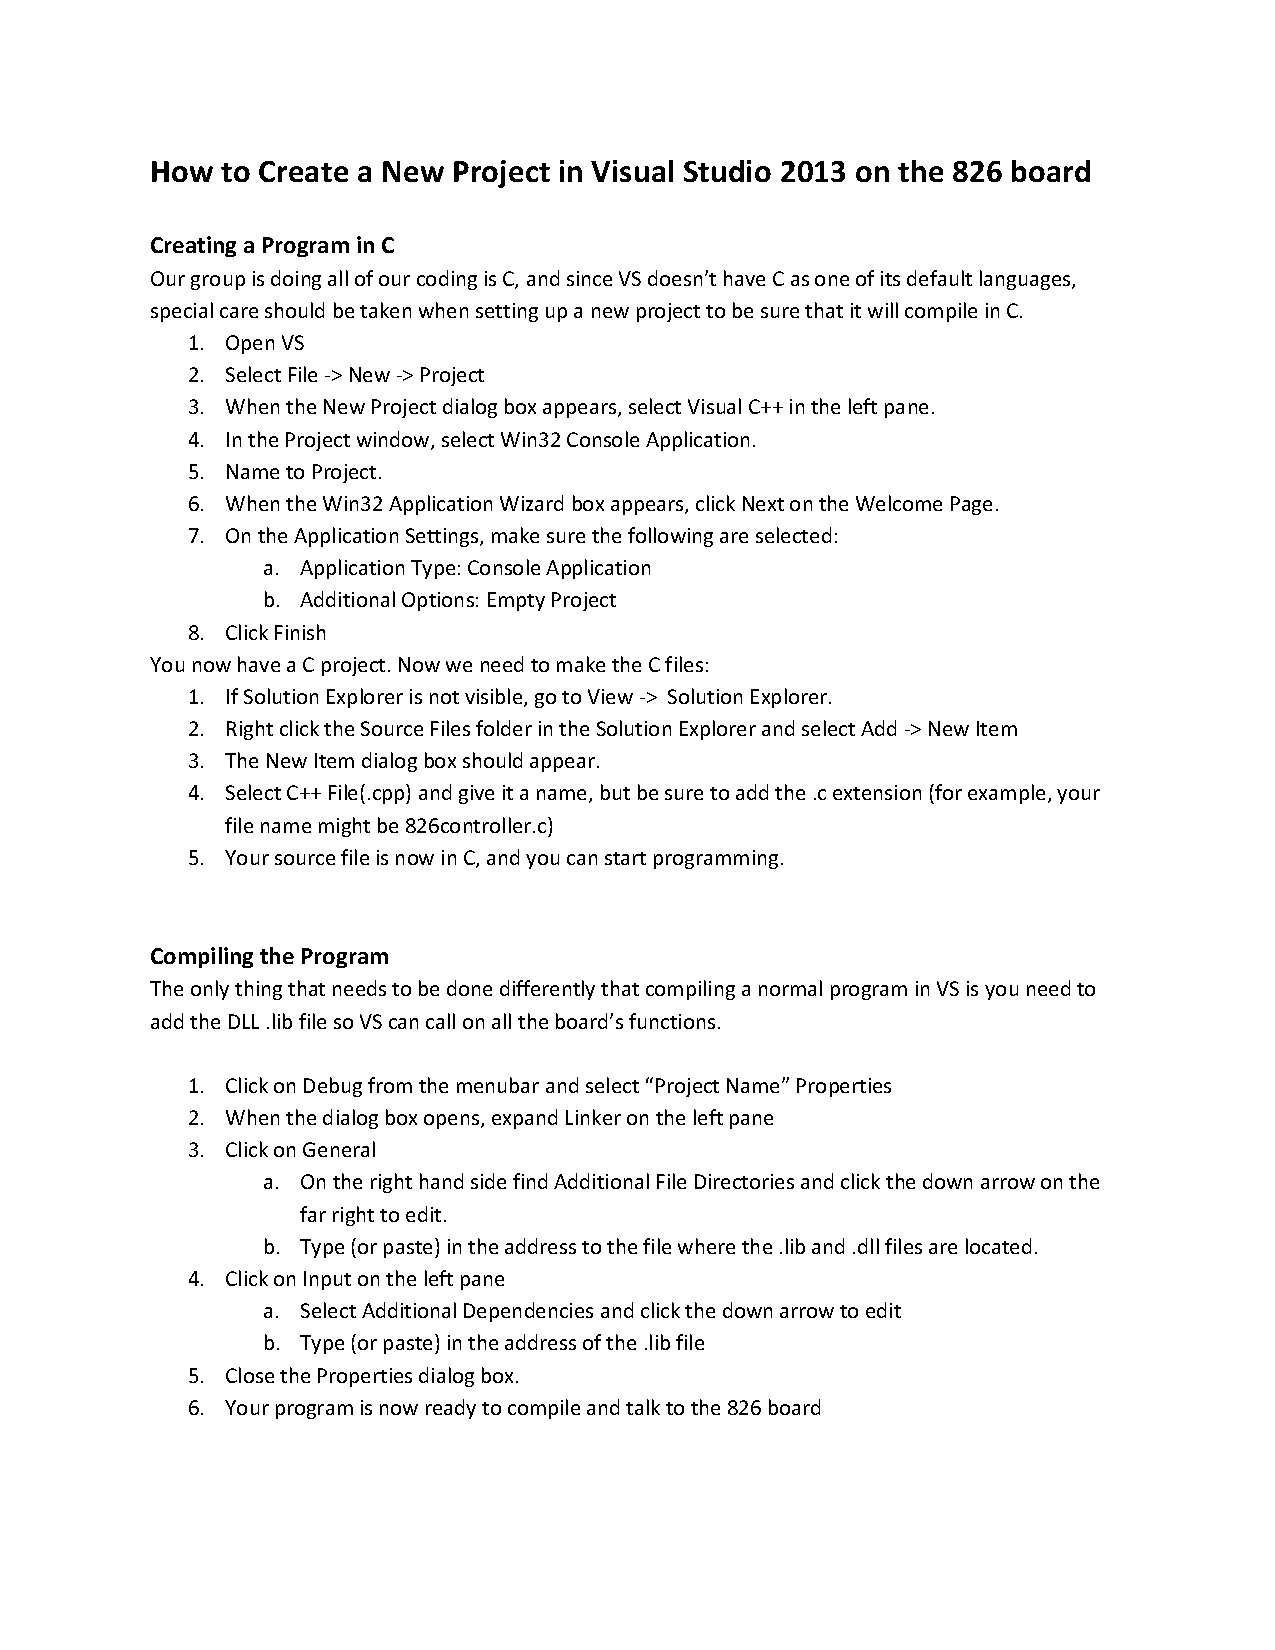
\includepdf[pages={-}]{visual.pdf}


\subsection*{Appendix D: Stepper Motor and Driver}
\addcontentsline{toc}{section}{Appendix D}



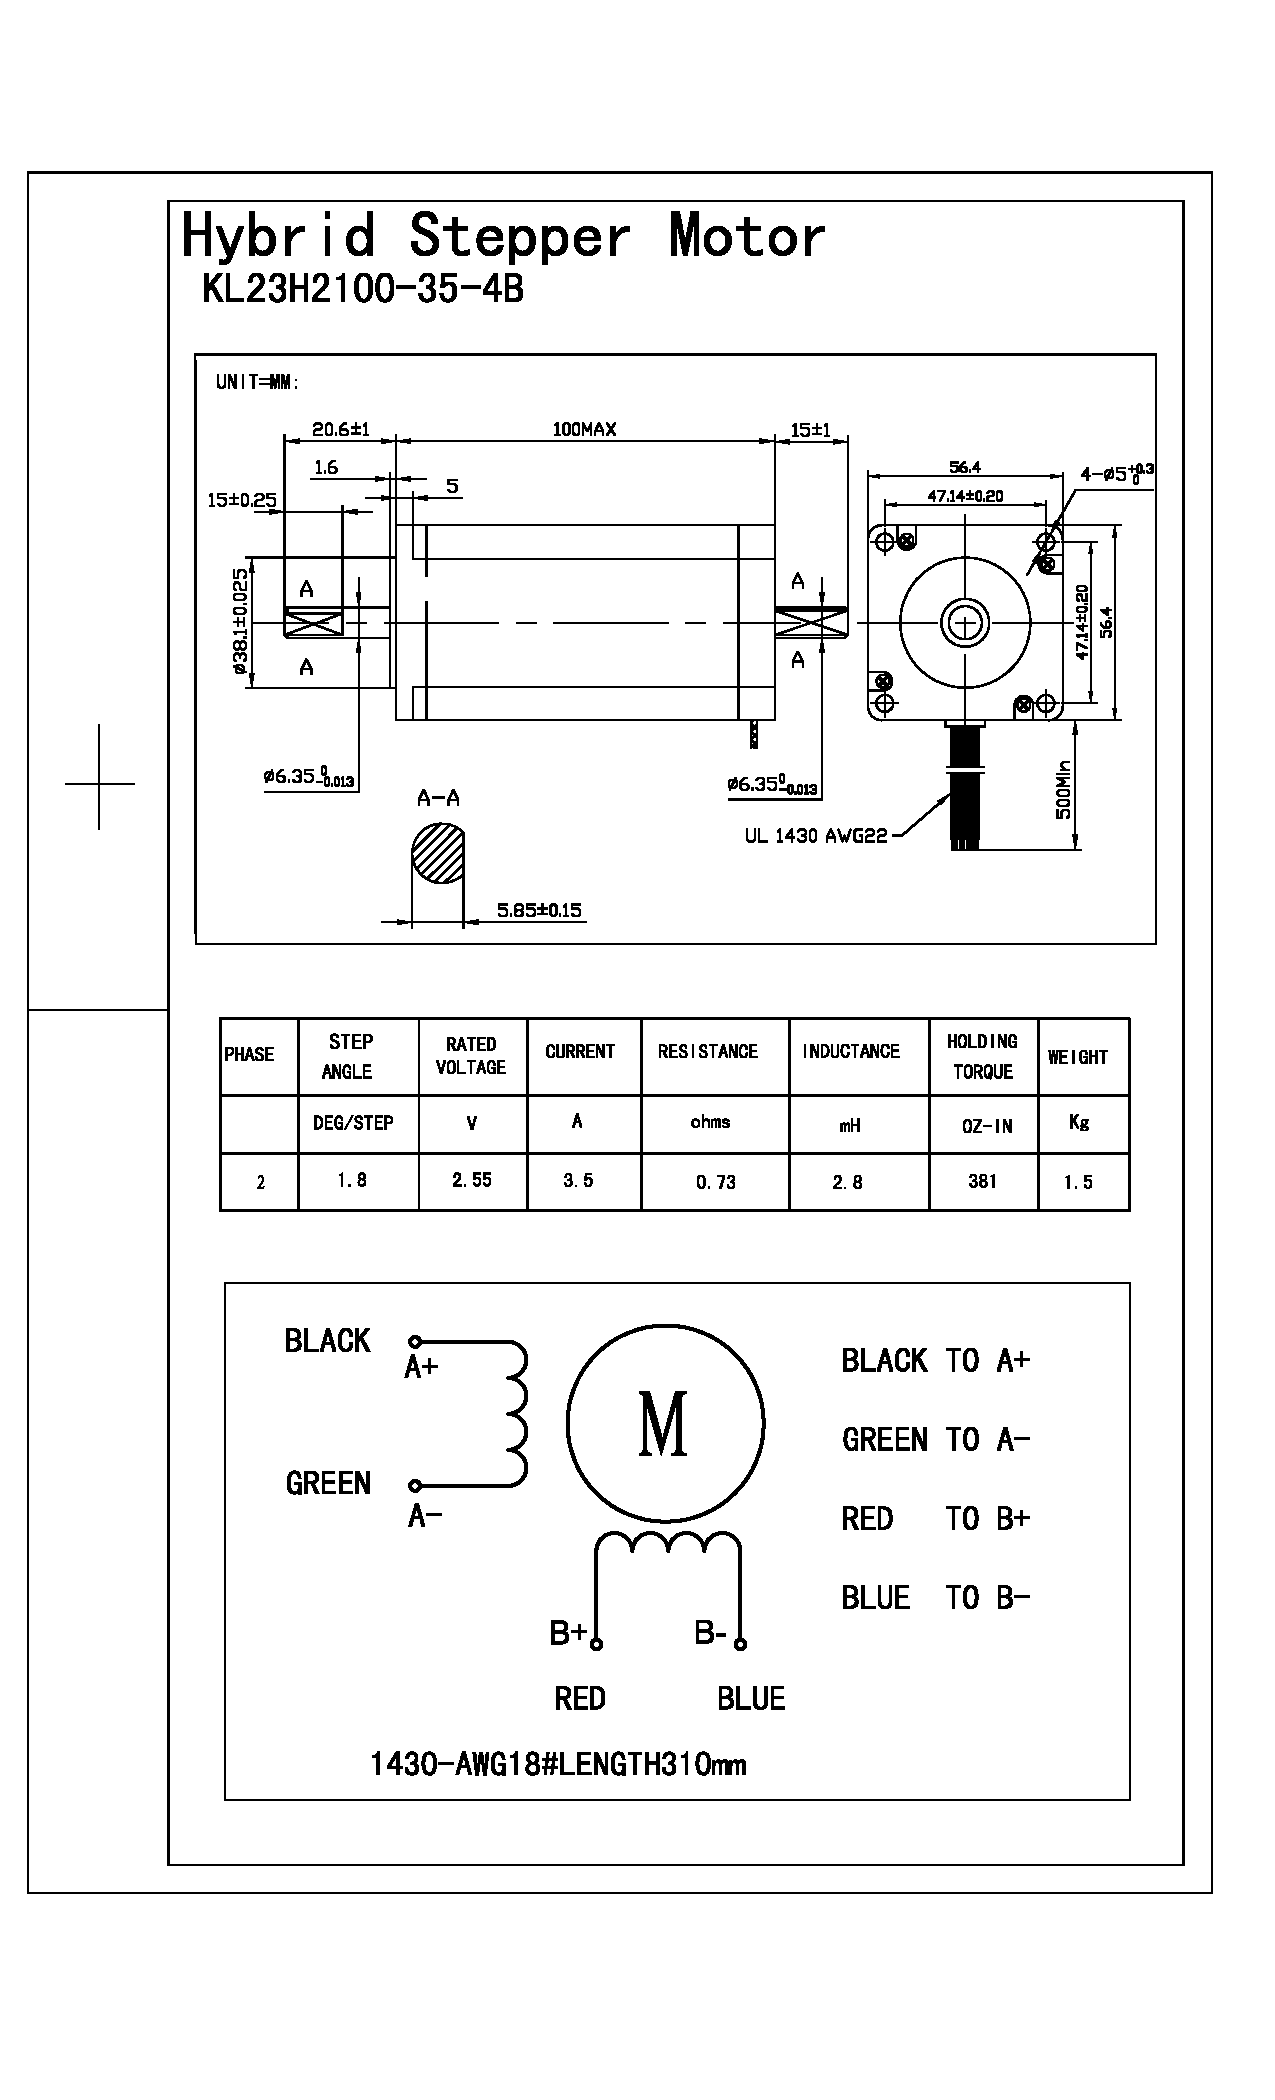
\includepdf[pages={-}]{hybrid.pdf}

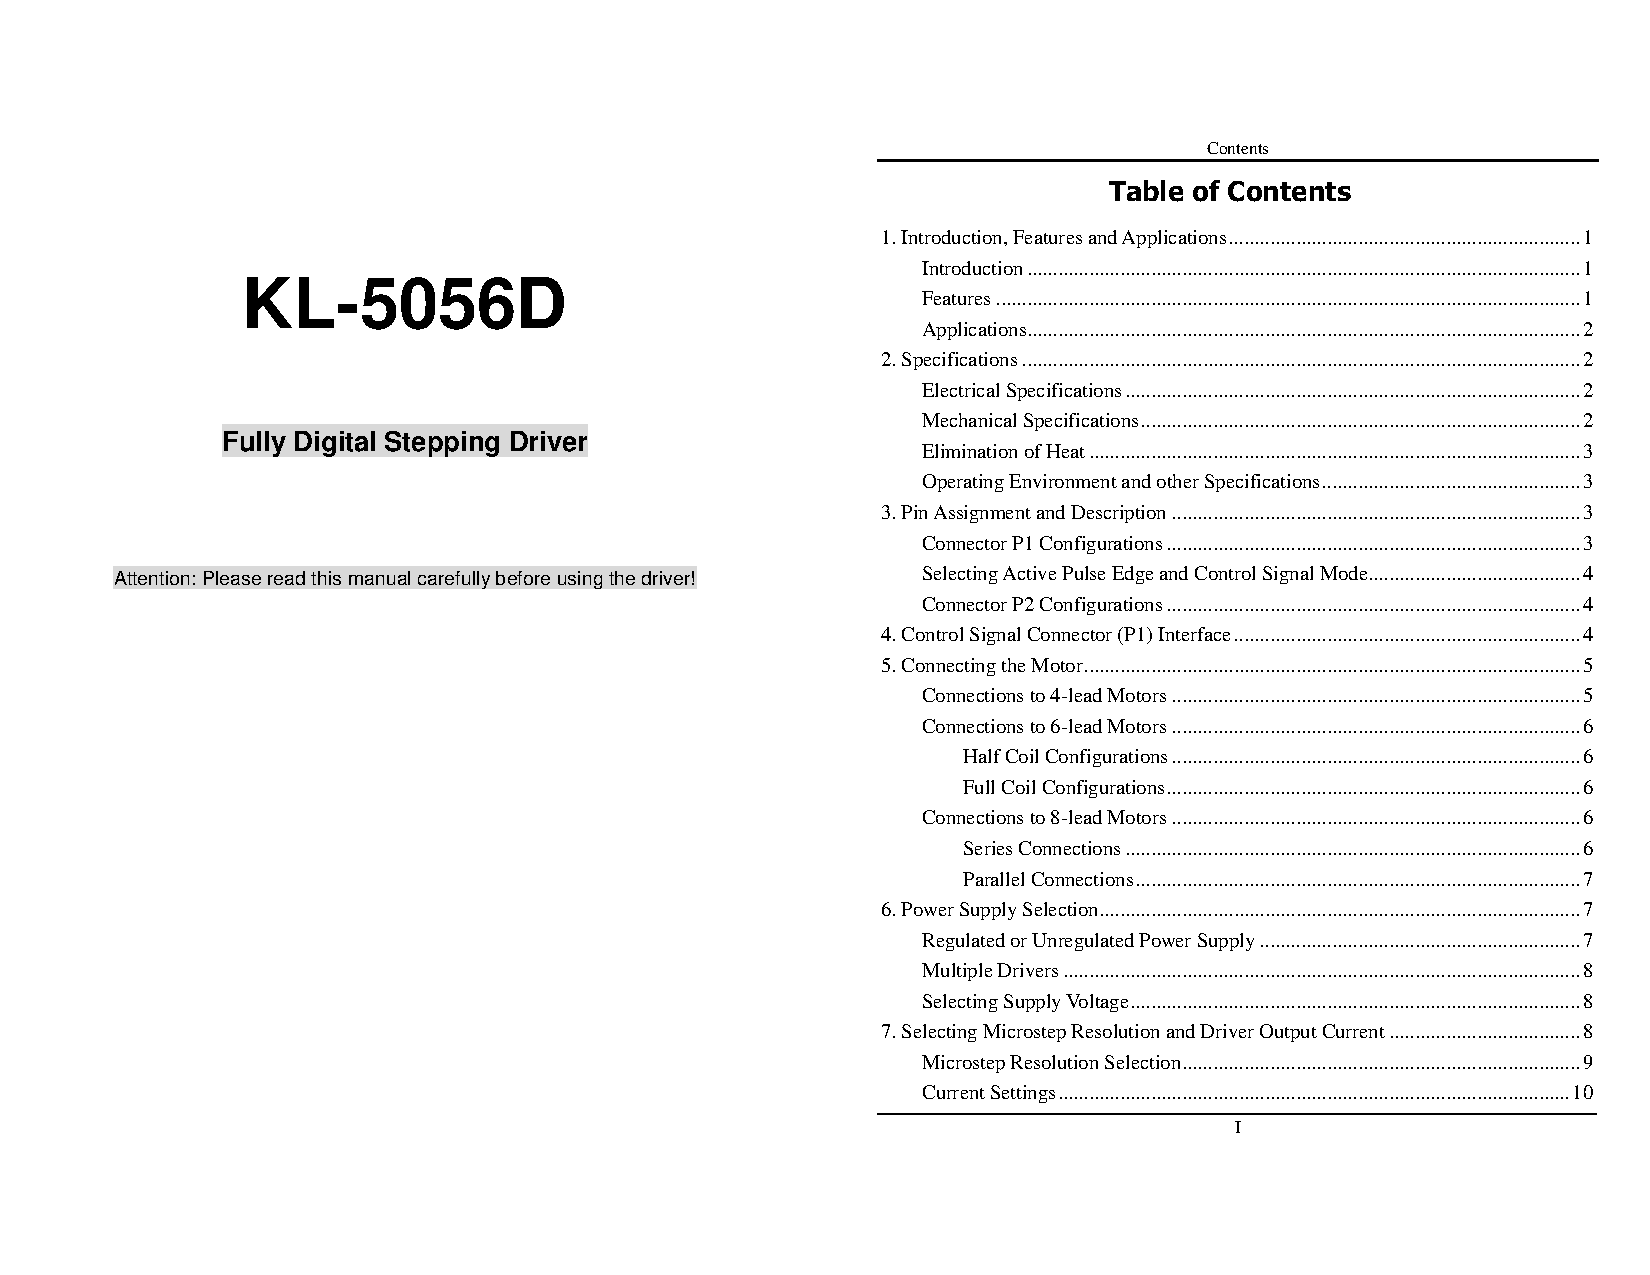
\includepdf[pages={-}]{driver.pdf}


\subsection*{Appendix E: Optical Shaft Encoder}
\addcontentsline{toc}{section}{Appendix E}

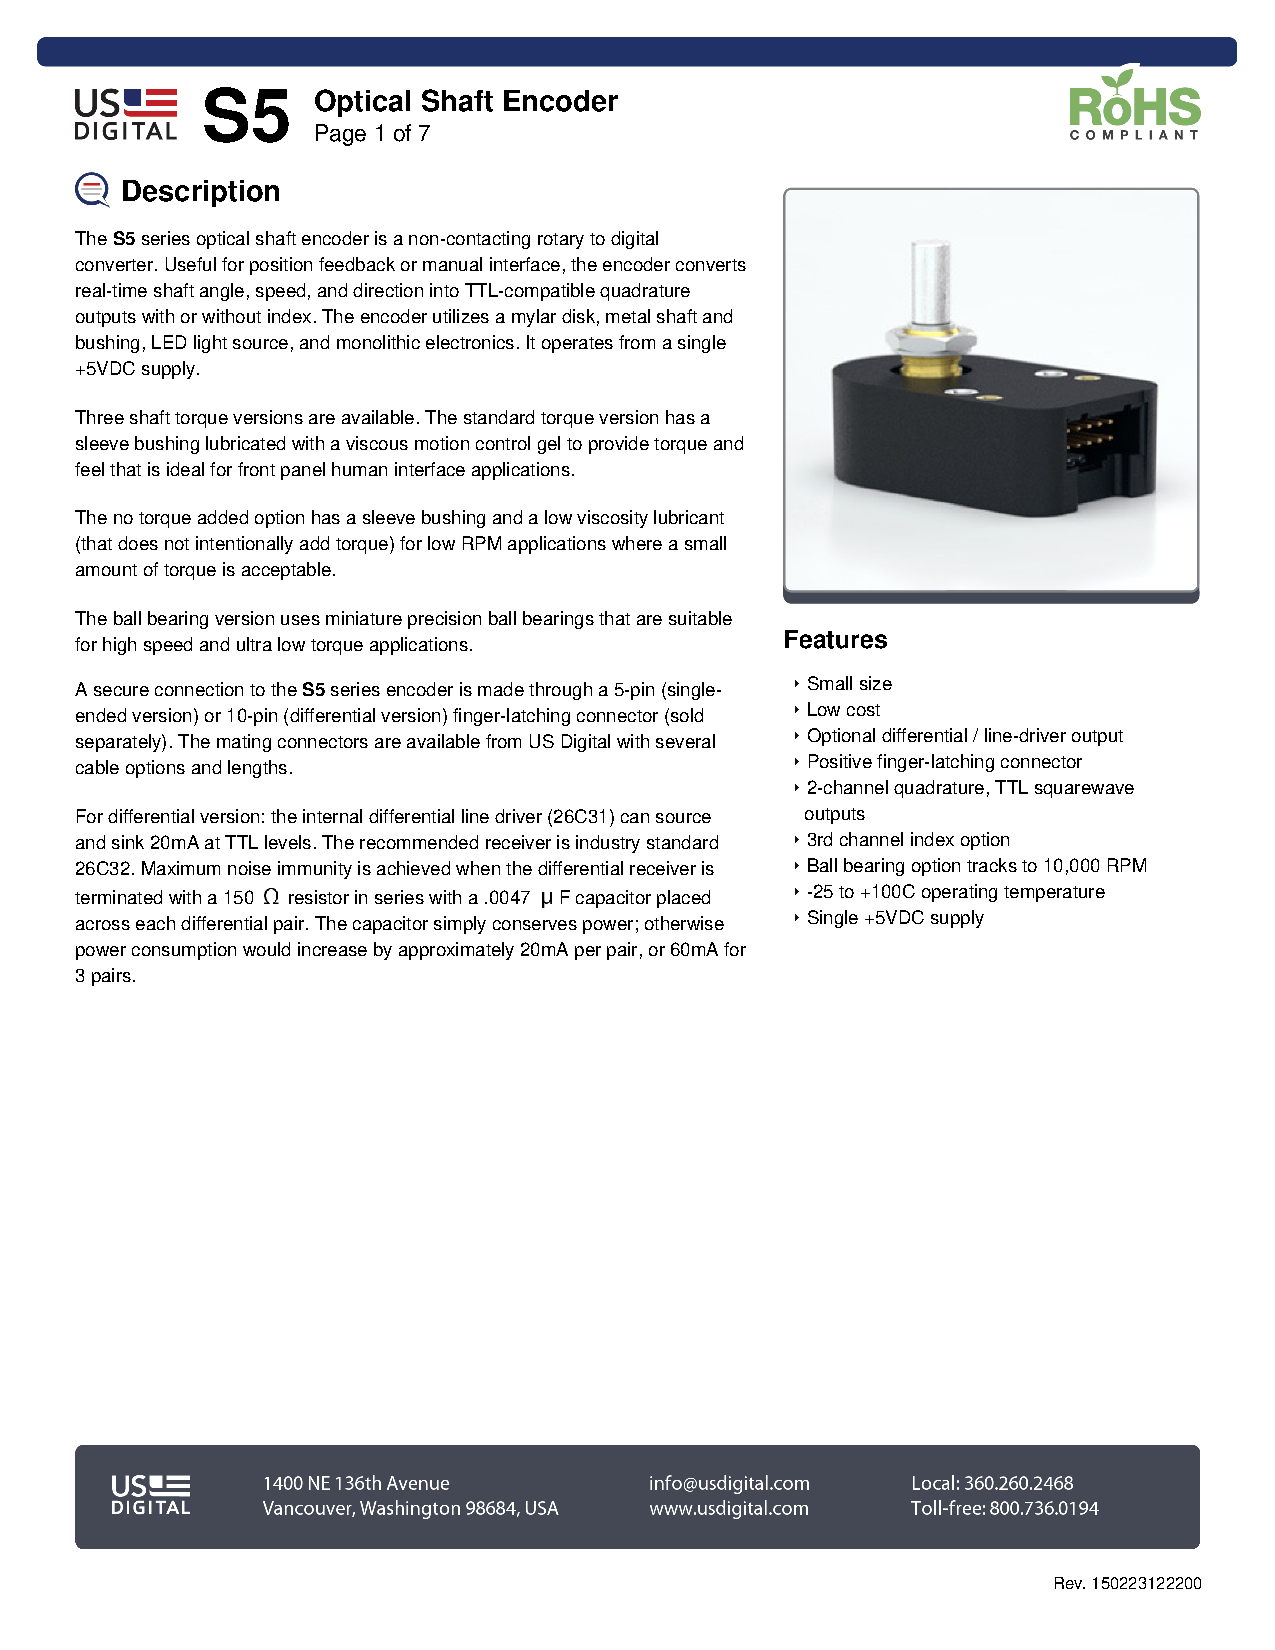
\includepdf[pages={-}]{optical.pdf}


\end{document}